\chapter{Design}

\section{Overall System Design}

\subsection{Short description of the main parts of the system}

\begin{itemize}
	\item \textbf{GCSE Trigonometry and Pythagoras Education System:}
	\begin{itemize}
		\item General User Interface
		\item Getting Username and Password
		\item Navigating User's Personal Account User Interface
		\item Setting Homework From Administrator
		\item Running Individual Lessons
		\item Running Individual Homeworks
		\item Accepting User Inputs
		\item Outputting Error Exception Messages
		\item Recording Homework Results On Database
		\item Viewing Results in Database
	\end{itemize}
\end{itemize}

\begin{itemize}
	\item General User Interface
	\begin{itemize}
		\item This is the general layout of the interface across the system; the same layout pattern, same colour scheme, same positioning design.
		\item This will provide the user with the ability to navigate the parts of the system that they have access to, and enable them to select tasks, submit homeworks, and access the database to view their personal and homework records.
	\end{itemize}
\end{itemize}

\begin{itemize}
	\item Getting Username and Password
	\begin{itemize}
		\item This will come in the very first window every time the user or administrator wants to access the program; it will ask them to log in so that they can view their own personal account, with all of their homework progress and personal records.
		\item It will mainly consist of two text boxes in the centre of the screen, one prompting a username and the other a password underneath. 
		\item If invalid information is input it will display an error message asking the user to retry. There will be no limit to the number of attempts a user can have; it won't lock them out of their computer if they keep getting it wrong.
	\end{itemize}
\end{itemize}

\begin{itemize}
	\item Navigating User's Personal Account User Interface
	\begin{itemize}
		\item This is essentially the functionality between each window. The user will have a range of buttons to press which will then open the relevant window, and then will have the option to return, making each part of the system accessible.
	\end{itemize}
\end{itemize}

\begin{itemize}
	\item Setting Homework From Administrator
	\begin{itemize}
		\item The function which makes the user aware of which homework has been set; the administrator will set it, the system will acknowledge it, and then notify the required users to do it.
		\item The reverse will work similarly; the user will complete the homework and the administrator will be notified. They will also be notified if the user hasn't completed it before the due date.
	\end{itemize}
\end{itemize}

\begin{itemize}
	\item Running Individual Lessons
	\begin{itemize}
		\item The module that runs for each lesson. Each lesson will have its own set of windows, containing the inputs, outputs and graphics to accurately represent what is being taught e.g Pythagoras Theorem.
		\item These will only be opened, navigated and closed as nothing from these is recorded in the database; they are effectively read only.
	\end{itemize}
\end{itemize}

\begin{itemize}
	\item Running Individual Homeworks
	\begin{itemize}
		\item The module that runs for each homework, saved so that each different homework task is always the same, in order to avoid confusion. 
		\item When the homework is run, inputs are accepted, outputs are given, and at the end the appropriate information is recorded in the database.
	\end{itemize}
\end{itemize}

\begin{itemize}
	\item Accepting User Inputs
	\begin{itemize}
		\item Each input type in the system, be it the general user interface, a lesson or a homework, will be accepted.
		\item Once accepted, it will be validated, and if invalid, the appropriate error message will be displayed.
		\item Different types of inputs are:
		\begin{itemize}
			\item Text Boxes
			\item Drag and Drop Images
			\item Image Modification
			\item Buttons 
		\end{itemize} 
		\item If valid, the system will either allow them access to their account, or add a mark to their homework task score.
	\end{itemize}
\end{itemize}

\begin{itemize}
	\item Outputting Error Exception Messages
	\begin{itemize}
		\item If a user's input is invalid, the appropriate error message will be displayed.
		\item Each error message will appear for 5 seconds and then disappear automatically.
		\item These are the variations of error messages and their causes:
		\begin{itemize}
			\item Invalid Username
			\item Invalid Password
			\item Invalid Data Type
			\item Wrong Answer 1{$^s$}{$^t$}
			\item Wrong Answer 2{$^n$}{$^d$}
			\item Unauthorised Access
		\end{itemize}
	\end{itemize}
\end{itemize}

\begin{itemize}
	\item Recording Homework Results On Database
	\begin{itemize}
		\item Every time a user completes a homework, the results will be recorded in the database, including the \textbf{OverallPercentScore}, \textbf{IndividualPercentScore(s)}, and \textbf{Rating}. 
		\item The user will be able to view their results in their personal database section, and the administrator will be able to view these results in the entire class database for that task.
	\end{itemize}
\end{itemize}

\begin{itemize}
	\item Viewing Results in Database
	\begin{itemize}
		\item A student will be able to click a button on the home screen to take them to the database view, where they will clearly see all of their personal results
		\item A teacher will be able to click a button on the home screen to take them to the database view, where they will clearly see all of the students results in any of their own classes, and they will be able to scroll through each student in alphabetical order on a scroll bar on the side to find individual's results
		\item An administrator (teacher) can amend a database value if it is necessary, although it is unlikely that it will be
		\item A return button will take them straight back to the home page to continue using the system
	\end{itemize}
\end{itemize}

\subsection{System flowcharts showing an overview of the complete system}

\textbf{This flowchart represents the system accessible for a student/user: }

%C:/Users/Jordan/git/COMP4Coursework2/Design/
%C:/Users/Jordan/git/COMP4Coursework2/Design

\begin{figure}[H]
    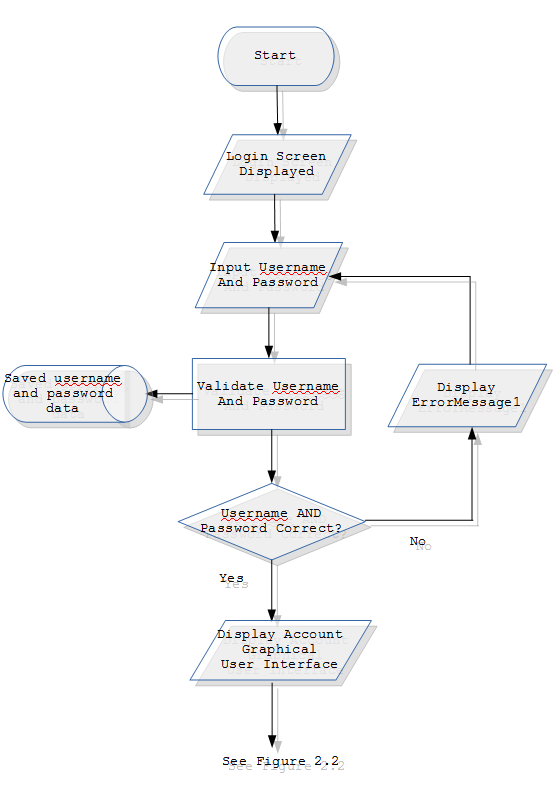
\includegraphics[width=\textwidth]{C:/Users/Jordan/git/COMP4Coursework2/Design/user_flow_1}
    \label{fig:print_function_result}\caption{}
\end{figure}

\begin{figure}[H]
    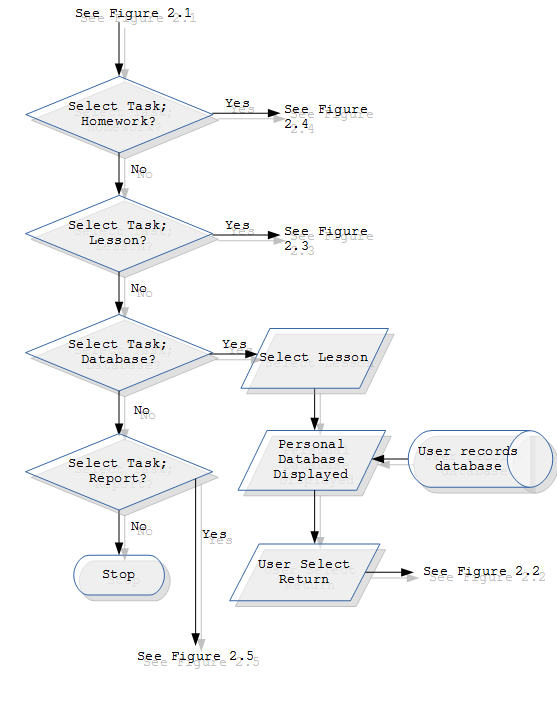
\includegraphics[width=\textwidth]{C:/Users/Jordan/git/COMP4Coursework2/Design/user_flow_2}
    \label{fig:print_function_result}\caption{}
\end{figure}

\begin{figure}[H]
    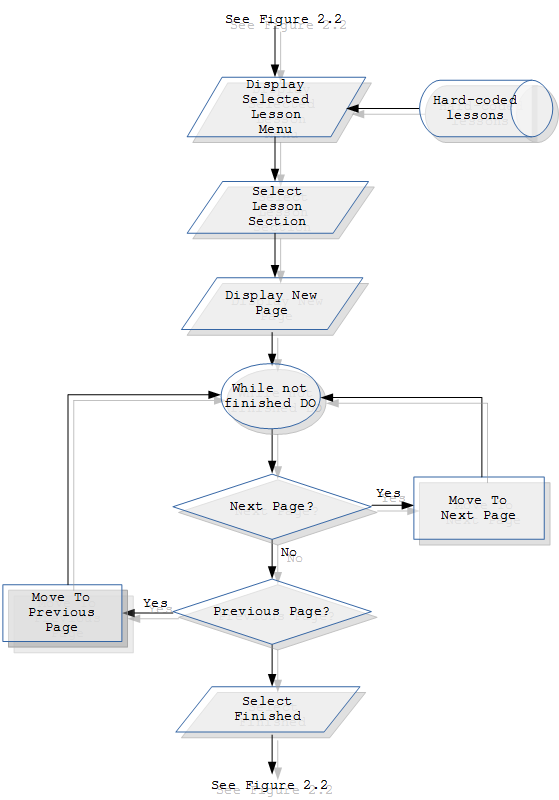
\includegraphics[width=\textwidth]{C:/Users/Jordan/git/COMP4Coursework2/Design/user_flow_3}
    \label{fig:print_function_result}\caption{}
\end{figure}

\begin{figure}[H]
    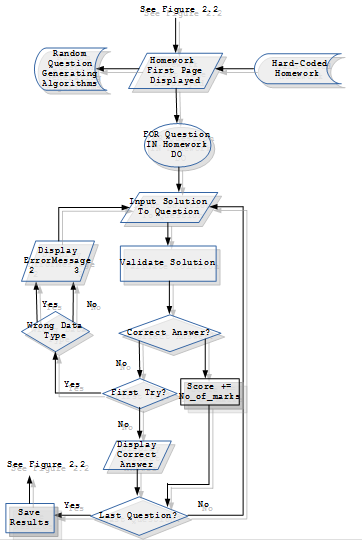
\includegraphics[width=\textwidth]{C:/Users/Jordan/git/COMP4Coursework2/Design/user_flow_4}
    \label{fig:print_function_result}\caption{}
\end{figure}

\textbf{This flowchart represents the system accessible for a teacher/administrator: }

\begin{figure}[H]
    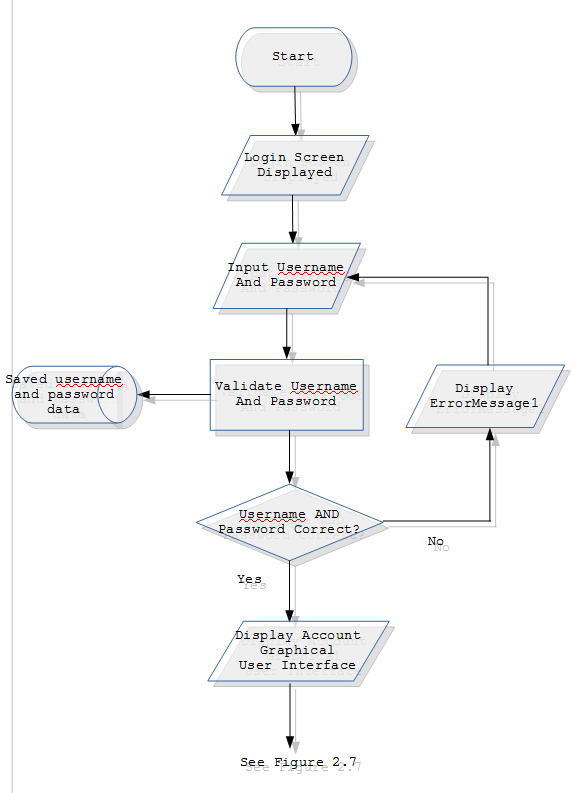
\includegraphics[width=\textwidth]{C:/Users/Jordan/git/COMP4Coursework2/Design/admin_flow_1}
    \label{fig:print_function_result}\caption{}
\end{figure}

\begin{figure}[H]
    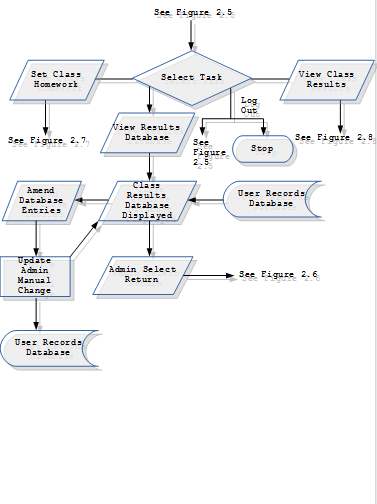
\includegraphics[width=\textwidth]{C:/Users/Jordan/git/COMP4Coursework2/Design/admin_flow_2}
    \label{fig:print_function_result}\caption{}
\end{figure}

\begin{figure}[H]
    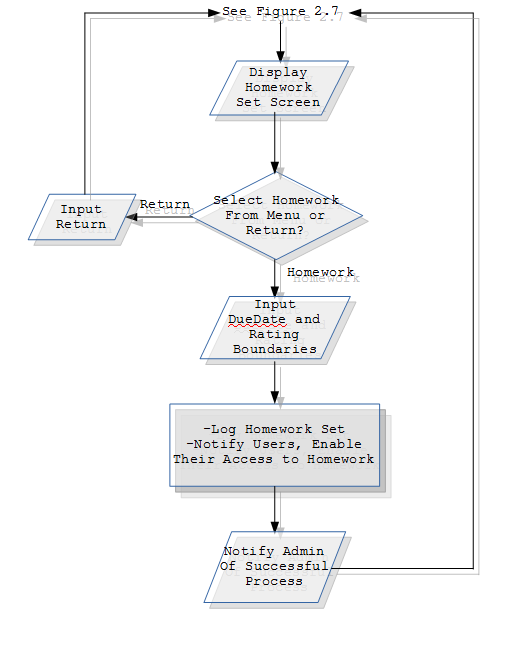
\includegraphics[width=\textwidth]{C:/Users/Jordan/git/COMP4Coursework2/Design/admin_flow_3}
    \label{fig:print_function_result}\caption{}
\end{figure}

\begin{figure}[H]
    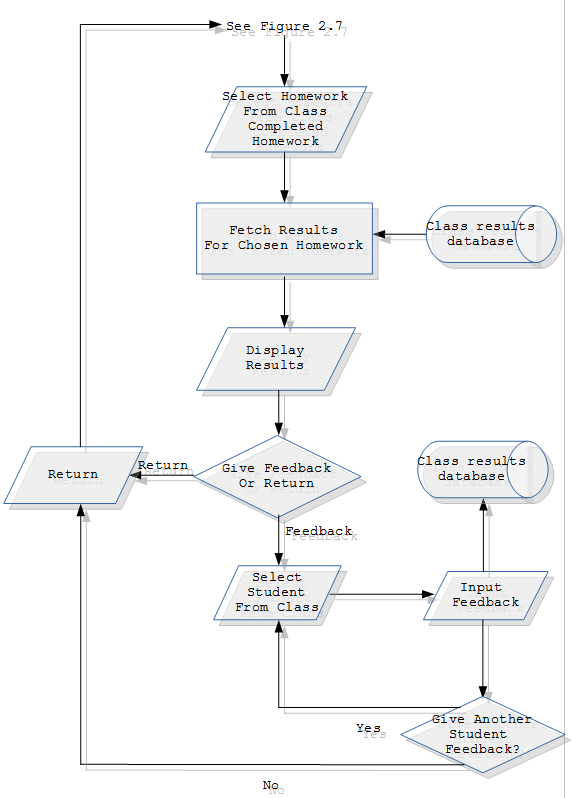
\includegraphics[width=\textwidth]{C:/Users/Jordan/git/COMP4Coursework2/Design/admin_flow_4}
    \label{fig:print_function_result}\caption{}
\end{figure}

\section{User Interface Designs}

%U:/git/COMP4Coursework2/Design
%C:/Users/Jordan/git/COMP4Coursework2/Design/

\begin{figure}[H]
    \label{fig:print_function_result}\caption{Login Screen}
    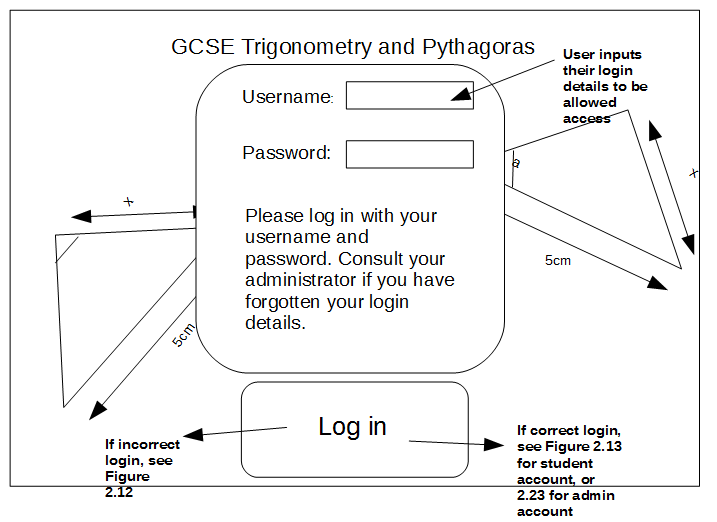
\includegraphics[width=\textwidth]{C:/Users/Jordan/git/COMP4Coursework2/Design/figure_2_9}
\end{figure}

\begin{figure}[H]
    \label{fig:print_function_result}\caption{ErrorMessage2}
    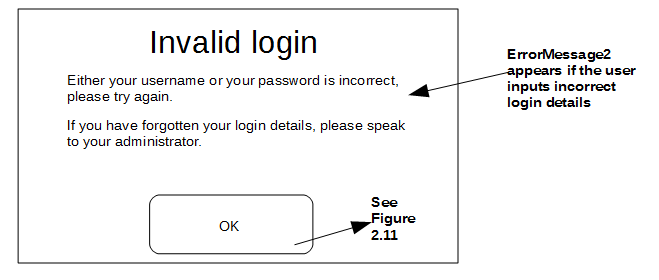
\includegraphics[width=\textwidth]{C:/Users/Jordan/git/COMP4Coursework2/Design/figure_2_10}
\end{figure}

\begin{figure}[H]
    \label{fig:print_function_result}\caption{Student Home Screen}
    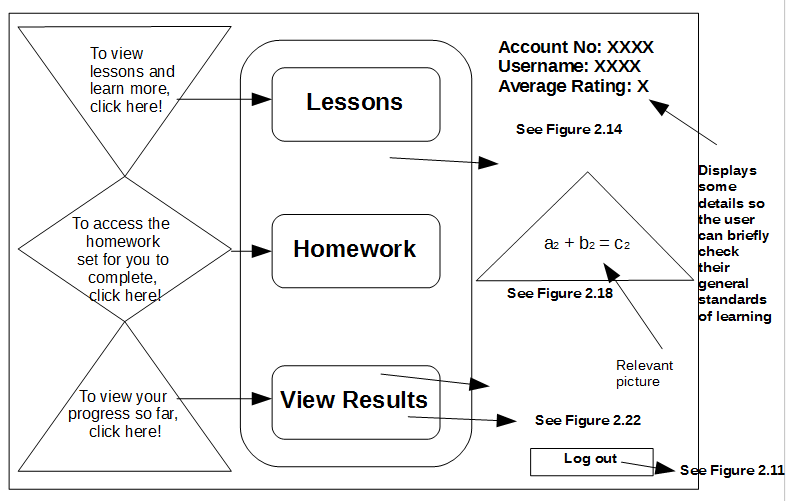
\includegraphics[width=\textwidth]{C:/Users/Jordan/git/COMP4Coursework2/Design/figure_2_11}
\end{figure}

\begin{figure}[H]
    \label{fig:print_function_result}\caption{Lesson Topic Menu}
    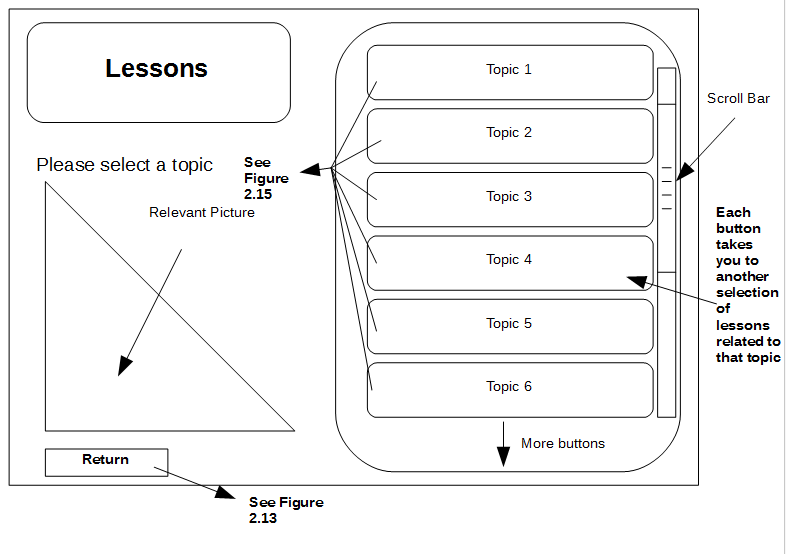
\includegraphics[width=\textwidth]{C:/Users/Jordan/git/COMP4Coursework2/Design/figure_2_12}
\end{figure}

\begin{figure}[H]
    \label{fig:print_function_result}\caption{Lesson Menu}
    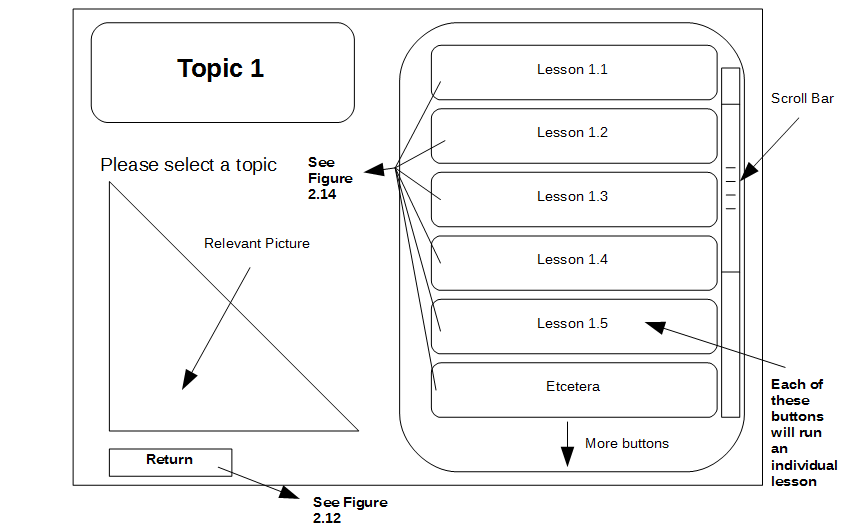
\includegraphics[width=\textwidth]{C:/Users/Jordan/git/COMP4Coursework2/Design/figure_2_13}
\end{figure}

\begin{figure}[H]
    \label{fig:print_function_result}\caption{First Lesson Screen}
    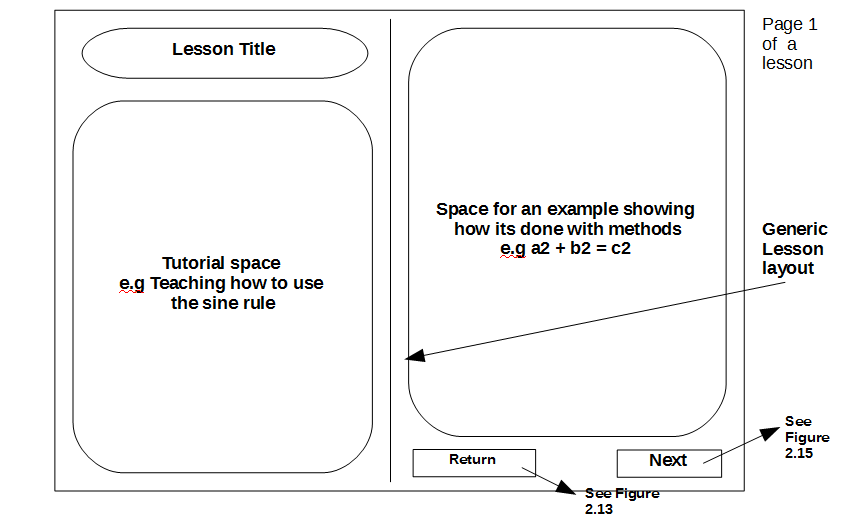
\includegraphics[width=\textwidth]{C:/Users/Jordan/git/COMP4Coursework2/Design/figure_2_14}
\end{figure}

\begin{figure}[H]
    \label{fig:print_function_result}\caption{Second Lesson Screen}
    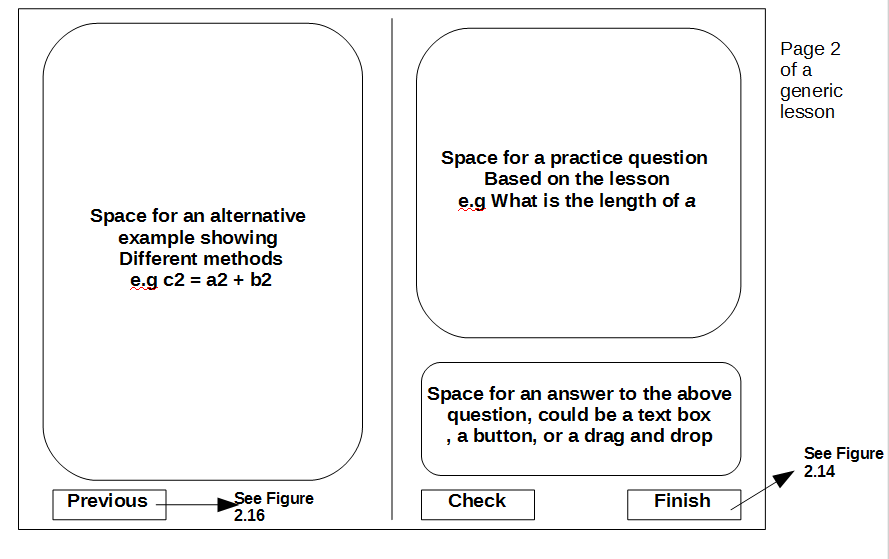
\includegraphics[width=\textwidth]{C:/Users/Jordan/git/COMP4Coursework2/Design/figure_2_15}
\end{figure}

\begin{figure}[H]
    \label{fig:print_function_result}\caption{Homework Topic Menu}
    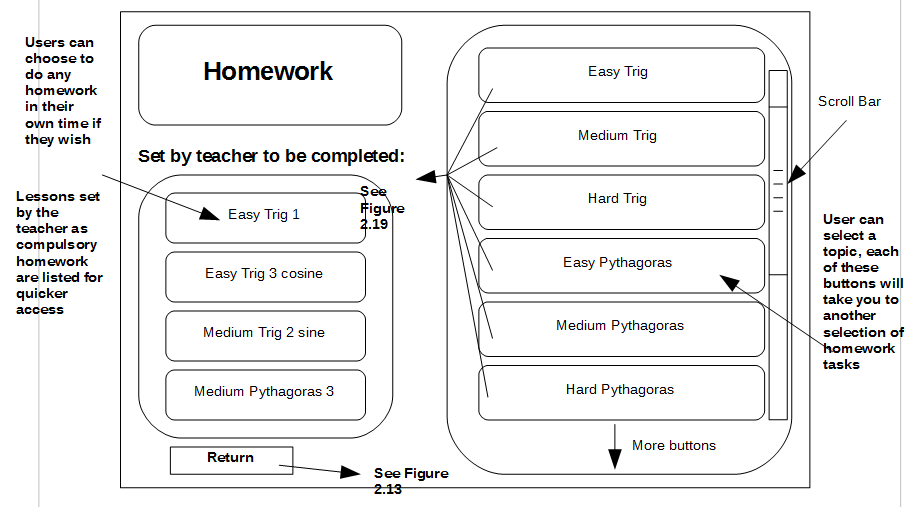
\includegraphics[width=\textwidth]{C:/Users/Jordan/git/COMP4Coursework2/Design/figure_2_16}
\end{figure}

\begin{figure}[H]
    \label{fig:print_function_result}\caption{Homework Menu}
    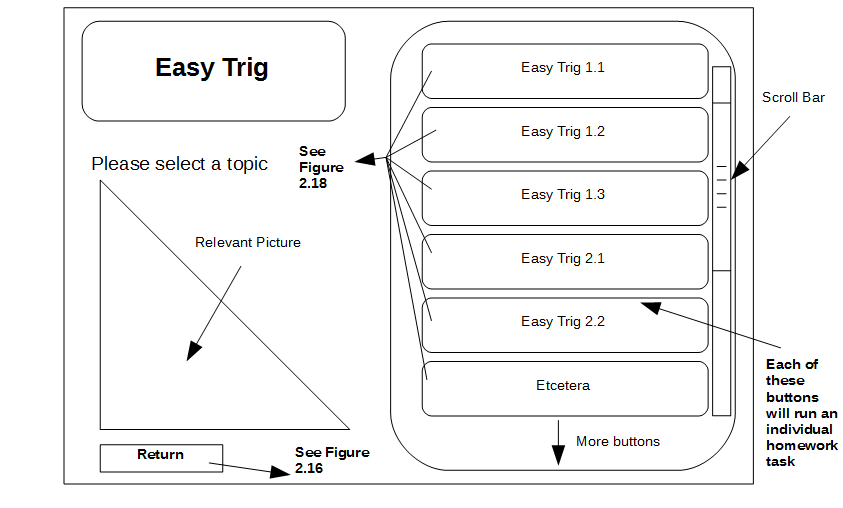
\includegraphics[width=\textwidth]{C:/Users/Jordan/git/COMP4Coursework2/Design/figure_2_17}
\end{figure}

\begin{figure}[H]
    \label{fig:print_function_result}\caption{First Homework Screen}
    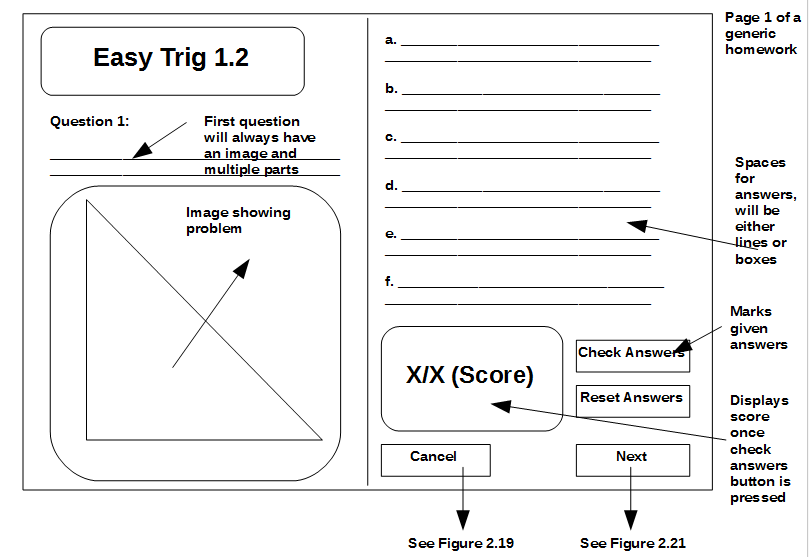
\includegraphics[width=\textwidth]{C:/Users/Jordan/git/COMP4Coursework2/Design/figure_2_18}
\end{figure}

\begin{figure}[H]
    \label{fig:print_function_result}\caption{Second Homework Screen}
    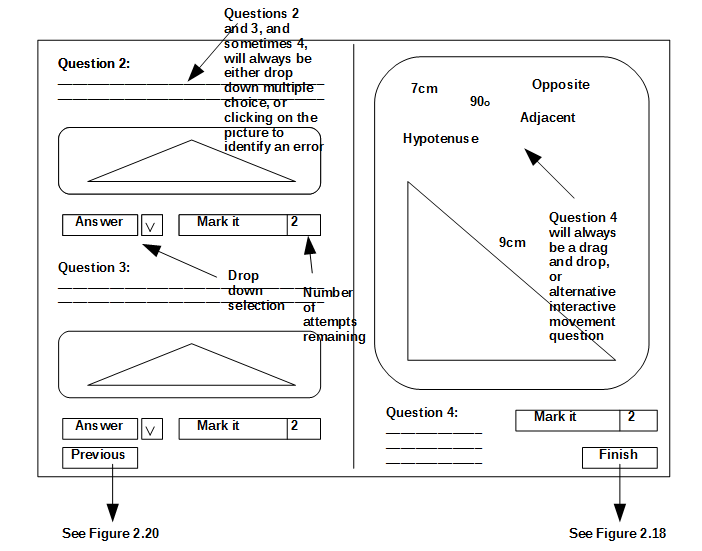
\includegraphics[width=\textwidth]{C:/Users/Jordan/git/COMP4Coursework2/Design/figure_2_19}
\end{figure}

\begin{figure}[H]
    \label{fig:print_function_result}\caption{Individual User Progress Database}
    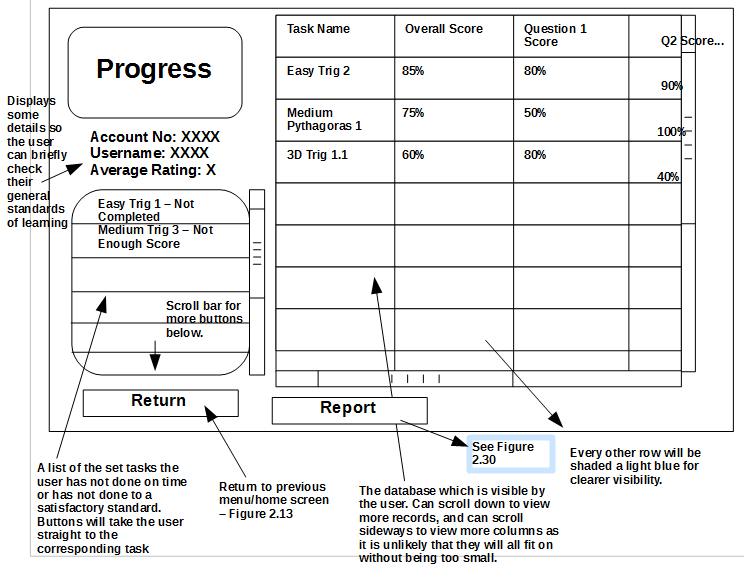
\includegraphics[width=\textwidth]{C:/Users/Jordan/git/COMP4Coursework2/Design/figure_2_20}
\end{figure}

\begin{figure}[H]
    \label{fig:print_function_result}\caption{Administrator Account Home}
    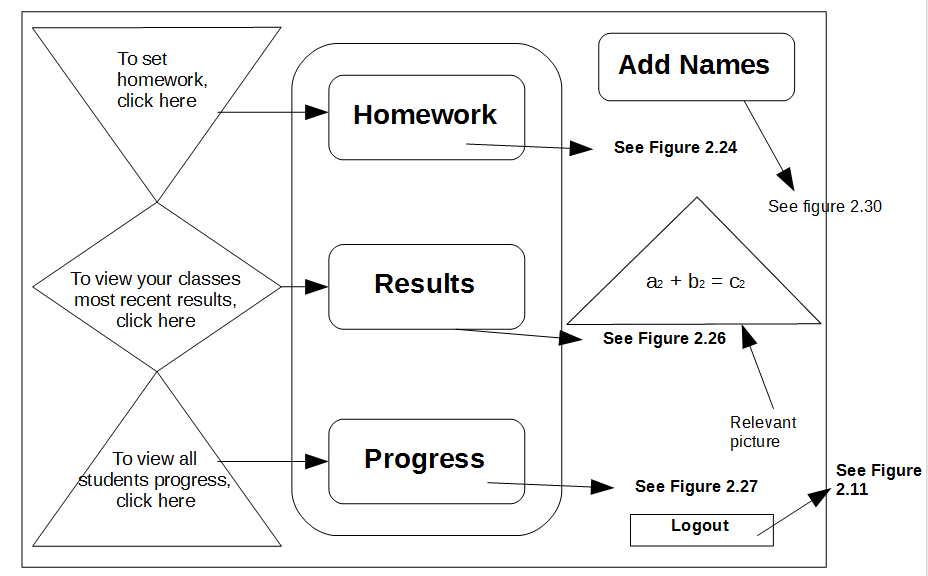
\includegraphics[width=\textwidth]{C:/Users/Jordan/git/COMP4Coursework2/Design/figure_2_21}
\end{figure}

\begin{figure}[H]
    \label{fig:print_function_result}\caption{Homework Setting Topic Menu}
    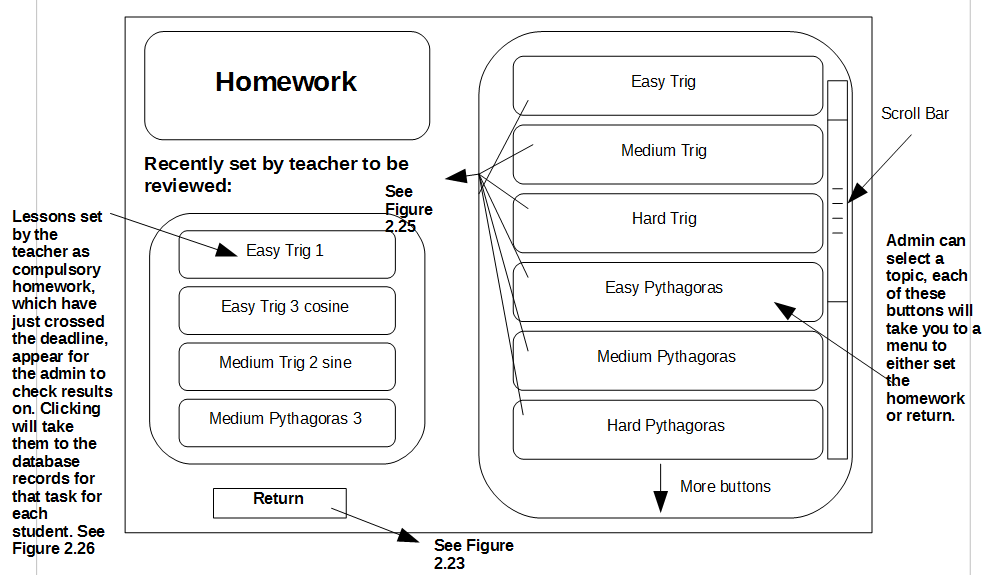
\includegraphics[width=\textwidth]{C:/Users/Jordan/git/COMP4Coursework2/Design/figure_2_22}
\end{figure}

\begin{figure}[H]
    \label{fig:print_function_result}\caption{Homework Set Screen}
    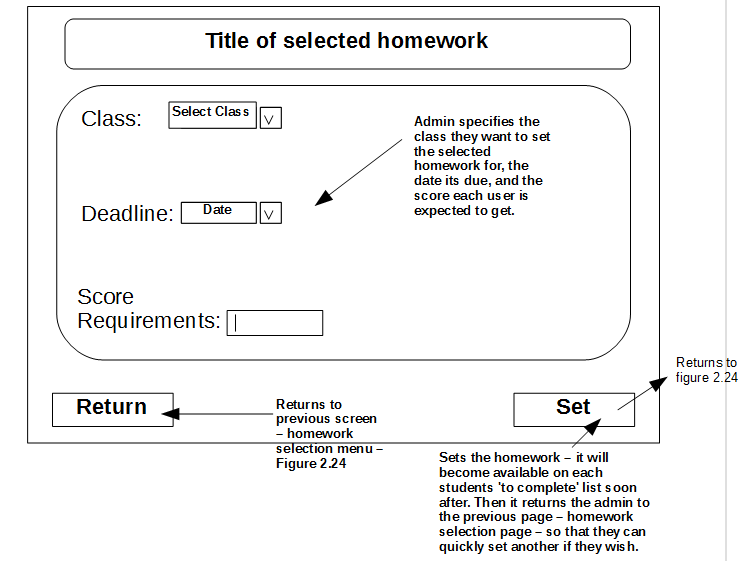
\includegraphics[width=\textwidth]{C:/Users/Jordan/git/COMP4Coursework2/Design/figure_2_23}
\end{figure}

\begin{figure}[H]
    \label{fig:print_function_result}\caption{Results Menu}
    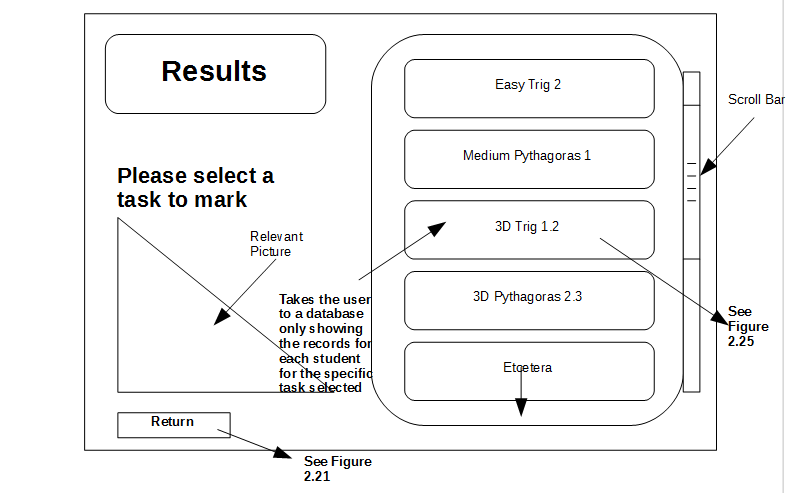
\includegraphics[width=\textwidth]{C:/Users/Jordan/git/COMP4Coursework2/Design/figure_2_24}
\end{figure}

\begin{figure}[H]
    \label{fig:print_function_result}\caption{Class Results Database}
    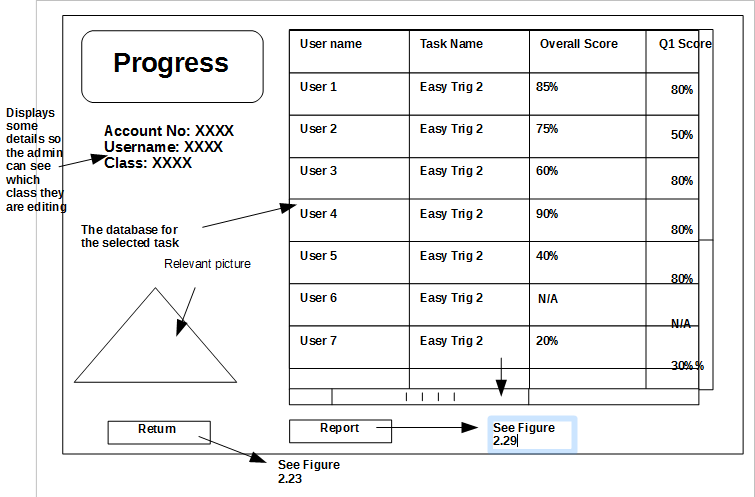
\includegraphics[width=\textwidth]{C:/Users/Jordan/git/COMP4Coursework2/Design/figure_2_25}
\end{figure}

\begin{figure}[H]
    \label{fig:print_function_result}\caption{ErrorMessage3}
    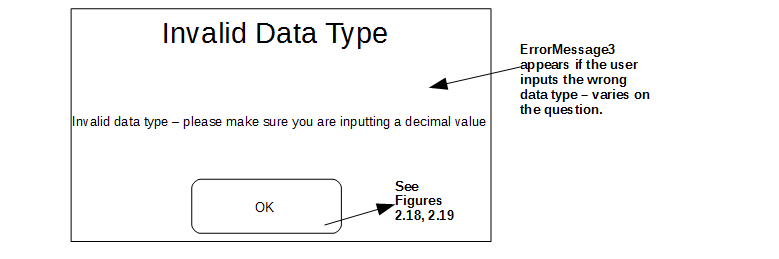
\includegraphics[width=\textwidth]{C:/Users/Jordan/git/COMP4Coursework2/Design/figure_2_26}
\end{figure}

\begin{figure}[H]
    \label{fig:print_function_result}\caption{ErrorMessage3}
    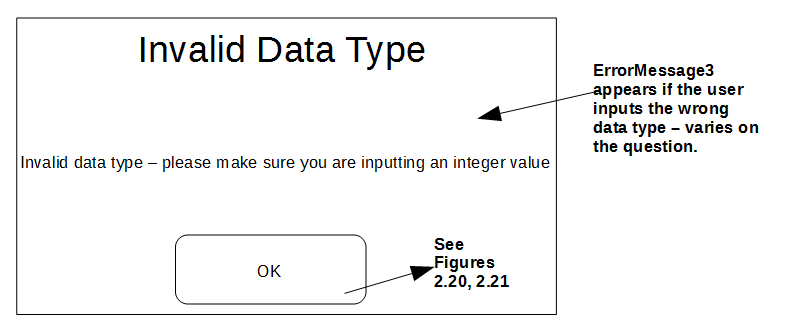
\includegraphics[width=\textwidth]{C:/Users/Jordan/git/COMP4Coursework2/Design/figure_2_27}
\end{figure}

\begin{figure}[H]
    \label{fig:print_function_result}\caption{ErrorMessage3}
    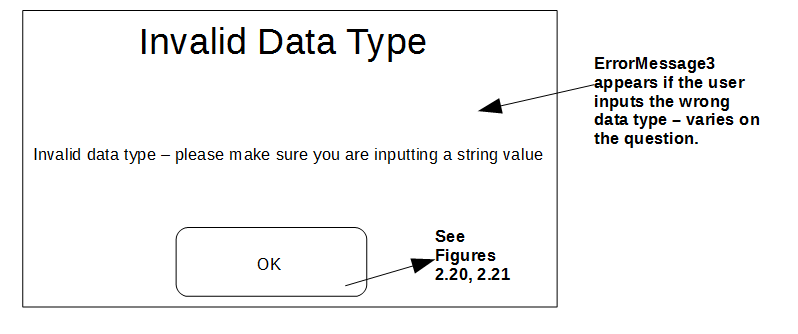
\includegraphics[width=\textwidth]{C:/Users/Jordan/git/COMP4Coursework2/Design/figure_2_28}
\end{figure}

\begin{figure}[H]
    \label{fig:print_function_result}\caption{ErrorMessage4}
    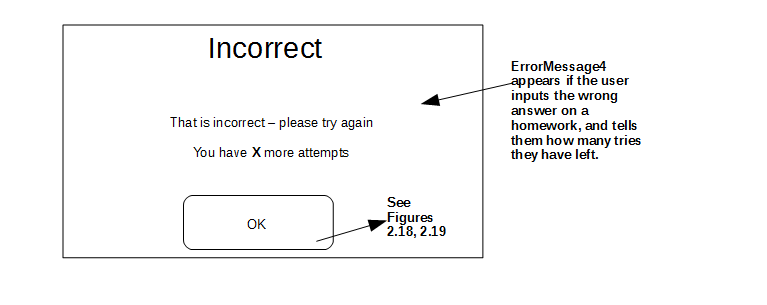
\includegraphics[width=\textwidth]{C:/Users/Jordan/git/COMP4Coursework2/Design/figure_2_29}
\end{figure}

\section{Hardware Specification}

This system will need to run on a standard desktop computer, as generally found in schools, using the Windows 7 operating system. It will need to have a screen resolution of 1920 x 1080, a 32 bit true colour scheme, a 16:9 aspect ratio, and an Intel HD Graphics 2500 card or better, running at 60p Hz. Windows 7 is required as it is still currently the operating system used by more or less every education facility, and the client will be working at such a facility. The 32 bit true colour scheme is usually the default set by the administrators, and they need a 16:9 aspect ratio, as I need to be able to make the windows fit properly on every machine at the facility, and the screens will not be resizable. The 1920 x 1080 resolution is desirable but not entirely necessary; it is achievable and will maintain the quality of the appearance of the program. The Intel HD Graphics 2500 is standard and should be able to run the system. A keyboard will be required for inputting text answers into boxes throughout the lessons, homework, and for logging in; any standard keyboard will be usable for this. Similarly, any standard mouse will be needed for navigating the GUI, clicking buttons, scrolling, using frop down boxes and dragging and dropping. A standard display will be used for the output of the system; just visual, no audio. The data for each user will be stored on a local server so that every user or administrator can view their own/all data from any of the machines at the facility. All of these requirements are able to be met by the client, who has it all available.

\section{Program Structure}

\subsection{Top-down design structure charts}

\begin{figure}[H]
    \label{fig:print_function_result}\caption{}
    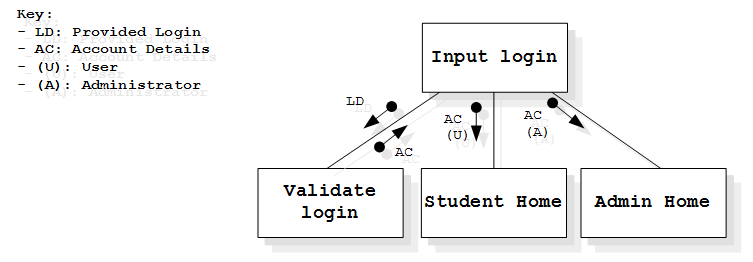
\includegraphics[width=\textwidth]{C:/Users/Jordan/git/COMP4Coursework2/Design/figure_2_30}
\end{figure}

\begin{figure}[H]
    \label{fig:print_function_result}\caption{}
    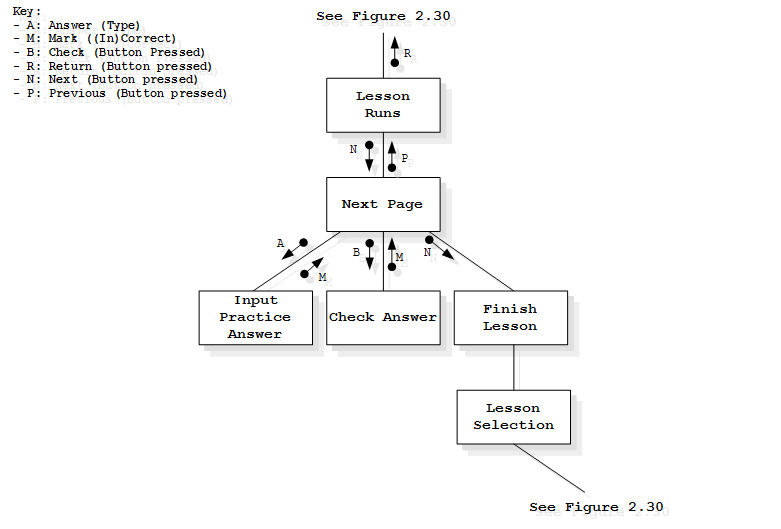
\includegraphics[width=\textwidth]{C:/Users/Jordan/git/COMP4Coursework2/Design/figure_2_31}
\end{figure}

\begin{figure}[H]
    \label{fig:print_function_result}\caption{}
    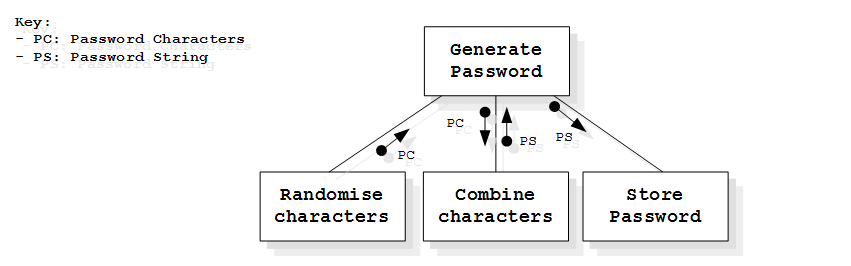
\includegraphics[width=\textwidth]{C:/Users/Jordan/git/COMP4Coursework2/Design/figure_2_32}
\end{figure}

\begin{figure}[H]
    \label{fig:print_function_result}\caption{}
    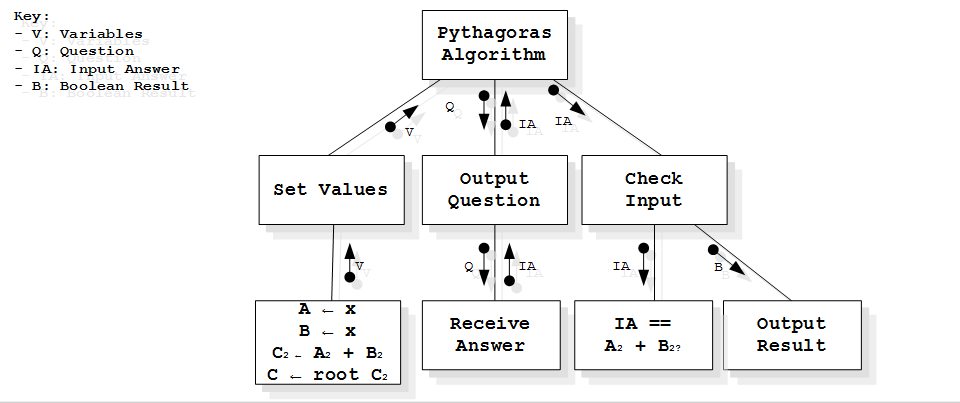
\includegraphics[width=\textwidth]{C:/Users/Jordan/git/COMP4Coursework2/Design/figure_2_33}
\end{figure}

\begin{figure}[H]
    \label{fig:print_function_result}\caption{}
    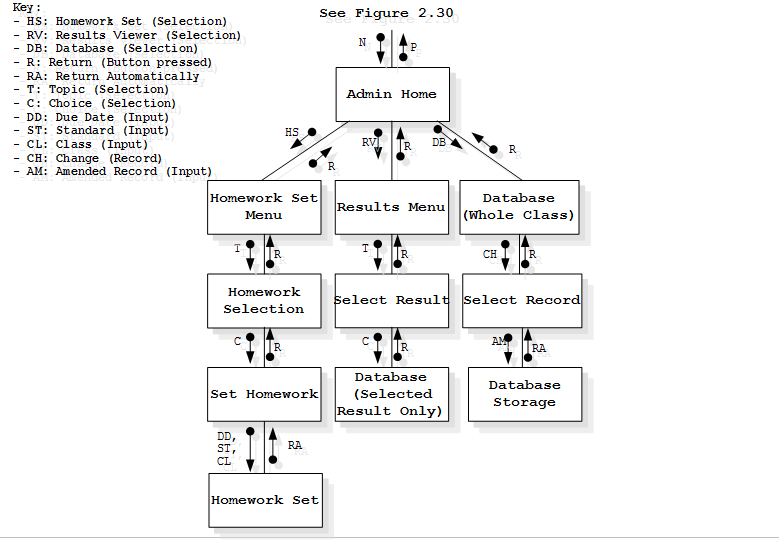
\includegraphics[width=\textwidth]{C:/Users/Jordan/git/COMP4Coursework2/Design/figure_2_34}
\end{figure}

\subsection{Algorithms in pseudo-code for each data transformation process}

\textbf{Validates the username and password when the user tries to log in:}

\begin{algorithm}[H]
\caption{Takes the logins from the database and adds them to a list from which they can be validated.}
\begin{algorithmic}[1]
\SET{$with \ open("logins.txt", mode = "r") as \ logins$}
\For{$name$}{$logins$}
	\SET{$list\_.append(name)$}
\EndFor
\RECEIVE{"Please enter your username"}
\SET{$return \ username$}
\RECEIVE{"Please enter your password"}
\SET{$return \ password$}
\SET{$count$}{$0$}
\SET{$found$}{$False$}
\While{$found = False$}{$and \ count < len(list\_)$}
	\If{$list\_[count] = str(username) \ and \ list\_[count + 2] = str(password)$}
		\SEND("Accepted")
		\SET{$found$}{$True$}
		\SET{$return \ found$}
	\Else{}
		\SEND{"Not accepted"}
		\SET{$call \ Validation$}
	\SET{$count \ += \ 1$}
	\EndIf
\EndWhile
\end{algorithmic}
\end{algorithm}

\begin{algorithm}[H]
\caption{Checks if the user's solution for the {$a^2 + b^2 = c^2$} is correct.}
\begin{algorithmic}[1]
\SET{$total\_marks$}{$0$}
\SET{$side\_a$}{$x$}
\SET{$side\_b$}{$x$}
\SET{$side\_c$}{$\sqrt{side\_a^2 + side\_b^2}$}
\SEND{$"Here \ is \ a \ right \ angled \ triangle. \ The \ length \ of \ side \ a \ is \ x$}
\SET{$centimetres, \ and \ the \ length \ of \ side \ b \ is \ x \ centimetres.$}
\SET{$Please \ calculate \ the \ length \ of \ side \ c"$}
\RECEIVE{$length$}{$"Please \ input \ the \ length \ of \ side \ c: "$}
\If {$length = side\_c$}
	\SEND{"+ 1 \ mark"}
	\SET{$total\_marks \ += \ x$}
\Else{}
	\SEND{"The \ answer \ is \ x"}
\EndIf
\end{algorithmic}
\end{algorithm}

\textbf{Alternative algorithm:}

\begin{algorithm}[H]
\caption{Same question and solution with a differently arranged formula.}
\begin{algorithmic}[1]
\SET{$total\_marks$}{$0$}
\SET{$side\_a$}{$x$}
\SET{$side\_b$}{$x$}
\SET{$side\_c^2$}{$side\_a^2 + side\_b^2$}
\SET{$side\_c$}{$\sqrt{side\_c^2}$}
\SEND{$"Here \ is \ a \ right \ angled \ triangle. \ The \ length \ of \ side \ a \ is \ x$}
\SET{$centimetres, \ and \ the \ length \ of \ side \ b \ is \ x \ centimetres.$}
\SET{$Please \ calculate \ the \ length \ of \ side \ c"$}
\RECEIVE{$length$}{$"Please \ input \ the \ length \ of \ side \ c: "$}
\If{$length = side\_c$}
	\SEND{"+ x \ marks"}
	\SET{$total\_marks \ += \ x$}
\Else{}
	\SEND{"The \ answer \ is \ x"}
\EndIf
\end{algorithmic}
\end{algorithm}

\textbf{3D Pythagoras algorithm:}

\begin{algorithm}[H]
\caption{Similar algorithm, but continues to check the user's solution for a 3D pythagoras problem.}
\begin{algorithmic}[1]
\SET{$total\_marks$}{$0$}
\SET{$left\_side\_a$}{$x$}
\SET{$middle\_side\_a$}{$x$}
\SET{$right\_side\_a$}{$x$}
\SET{$inside\_side\_a$}{$\sqrt{left\_side\_a^2 + middle\_side\_a^2}$}
\SET{$inside\_side\_b$}{$\sqrt{right\_side\_a^2 + inside\_side\_a^2}$}
\SEND{$"A \ magician \ stores \ his \ wand \ in \ a \ box.$}
\SET{$The \ box \ is \ xcm \ by \ xcm \ by \ xcm.$}
\SET{$The \ wand \ only \ just \ fits \ in \ wedged \ against \ opposite \ corners."$}
\RECEIVE{$length$}{$"How \ long \ is \ the \ wand?"$}
\If{$length = inside\_side\_b$}
	\SEND{"+ \ x \ marks"}
	\SET{$total\_marks \ += \ x$}
\Else{}
	\SEND{"The \ answer \ is \ x"}
\EndIf	
\end{algorithmic}
\end{algorithm}

\textbf{Trigonometry Algorithms:}

\begin{algorithm}[H]
\caption{Sine rule.}
\begin{algorithmic}[1]
\SET{$sinA$}{$\frac{opposite}{hypotenuse}$}{$\frac{a}{h}$}
\end{algorithmic}
\end{algorithm}

\begin{algorithm}[H]
\caption{Cosine rule.}
\begin{algorithmic}[1]
\SET{$cosA$}{$\frac{adjacent}{hypotenuse}$}{$\frac{b}{h}$}
\end{algorithmic}
\end{algorithm}

\begin{algorithm}[H]
\caption{Tan rule.}
\begin{algorithmic}[1]
\SET{$tanA$}{$\frac{opposite}{adjacent}$}{$\frac{a}{b}$}
\end{algorithmic}
\end{algorithm}

\begin{algorithm}[H]
\caption{The sine formula in use.}
\begin{algorithmic}[1]
\SET{$\frac{A}{sinA}$}{$\frac{B}{sinB}$}
\If{$\frac{A}{sinA} = \frac{B}{sinB}$}
	\SEND{"Your solution is correct"}
\Else{}
	\SEND{"Your solution is not correct"}
\EndIf
\end{algorithmic}
\end{algorithm}

\begin{algorithm}[H]
\caption{The cosine formula in use.}
\begin{algorithmic}[1]
\SET{$a^2$}{$b^2 + c^2 \ - \ 2bc \ cosA$}
\RECEIVE{$side\_a$}{$"Please \ input \ the \ length \ of \ side \ a: "$}
\If{$side\_a = {b^2 + c^2 - 2bc \ cosA}$}
	\SEND{"Correct"}
\Else{}
	\SEND{"Incorrect"}
\EndIf
\end{algorithmic}
\end{algorithm}

\begin{algorithm}[H]
\caption{The formula for finding angles in scalene triangles using the cosine rule.}
\begin{algorithmic}[1]
\SET{$cosA \ b^2 + c^2 - \frac{a^2}{2bc}$}
\SET{$C$}{$inv \ cos\frac{adjacent}{hypotenuse}$}
\RECEIVE{$angle\_c$}{$"Please \ input \ the \ size \ of \ angle \ C:"$}
\If{$angle\_c = {inv \ cos\frac{adjacent}{hypotenuse}}$}
	\SEND{"Correct"}
\Else{}
	\SEND{"Correct"}
\EndIf
\end{algorithmic}
\end{algorithm}

\begin{algorithm}[H]
\caption{Formula for finding the area of a scalene triangle using the sine rule.}
\begin{algorithmic}[1]
\SET{$area$}{$\frac{1}{2} \ ab \ sinC$}
\RECEIVE{$area\_1$}{"Please \ input \ the \ area \ of \ this \ scalene \ triangle:"}
\If{$area\_1 = \frac{1}{2} \ ab \ sinC$}
	\SEND{"Correct"}
\Else{}
	\SEND{"Incorrect"}
\EndIf
\end{algorithmic}
\end{algorithm}

\begin{algorithm}[H]
\caption{Formula for finding an angle using the tan rule.}
\begin{algorithmic}[1]
\SET{$tanA$}{$\frac{10}{15}$}
\SET{$\frac{10}{15}$}{$ \ $}{$0.67$}
\SET{$tan^-1(0.67)$}{$33.82^o$}
\SET{$tanA$}{$33.82^o$}
\RECEIVE{$tan\_a$}{"Please \ input \ the \ size \ of \ the \ angle \ using \ the \ tan \ rule:"}
\If{$tan\_a = {33.82^o}$}
	\SEND{"Correct"}
\Else{}
	\SEND{"Incorrect"}
\EndIf
\end{algorithmic}
\end{algorithm}

\textbf{Algorithm for resetting the answers on the homework: }

\begin{algorithm}[H]
\begin{algorithmic}[1]
\For{$question$}{$screen$}
	\SET{$question\_text\_box.value = 0$}
\EndFor
\end{algorithmic}
\end{algorithm}

\textbf{Algorithm for saving the results to the database: }

\begin{algorithm}[H]
\begin{algorithmic}[1]
\SET{$score\_percentage\_1$}{$75$}
\SET{$score\_percentage\_2$}{$50$}
\If{$button\_pressed = finish\_button$}
	\For{$question$}{$screen\_1$}
		\SET{$database.topic.percentage\_1.append$}{$score\_percentage\_1$}
	\EndFor
	\For{$question$}{$screen\_2$}
		\SET{$database.topic.percentage\_2.append$}{$score\_percentage\_2$}
	\EndFor
\EndIf
\end{algorithmic}
\end{algorithm}

\textbf{Algorithm for setting the homeworks: }

\begin{algorithm}[H]
\begin{algorithmic}[1]
\If{$button\_pressed = topic$}
	\SET{$set\_topic$}{$topic$}
\EndIf
\For{$student$}{$class$}
	\SET{$topic.activate$}
	\SEND{$You \ must \ now \ complete \ \{0\}.format\{topic\}$}
\EndFor 
\end{algorithmic}
\end{algorithm}

\subsection{Object Diagrams}

\begin{figure}[H]
    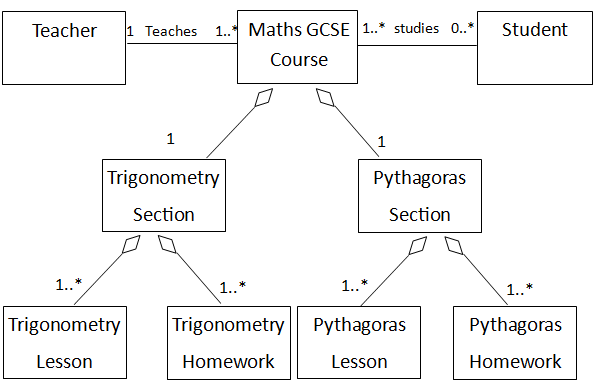
\includegraphics[width=\textwidth]{C:/Users/Jordan/git/COMP4Coursework2/Design/objectrelationships.png}
    \caption{The relationships between each of the objects in the proposed system} \label{fig:print_function_result}
\end{figure}

\subsection{Class Definitions}

\begin{center}
\begin{tabular}{|p{5cm}|} \hline
Course \\ \hline
Title \\
Subject \\ \hline
AddTitle \\ 
EditTitle \\
AddSubject \\
EditSubject \\ \hline
\end{tabular}
\end{center}

\begin{center}
\begin{tabular}{|p{5cm}|} \hline
Teacher \\ \hline
Surname \\
Title \\
Subject \\ \hline
AddSurname \\
EditSurname \\
AddTitle \\
EditTitle \\
AddSubject \\
EditSubject \\ \hline
\end{tabular}
\end{center}

\begin{center}
\begin{tabular}{|p{5cm}|} \hline
Student \\ \hline
FirstName \\
Surname \\
UserID \\
Password  \\ \hline
AddFirstName \\
EditFirstName \\
AddSurname \\
EditSurname \\
AddUserID \\
EditUserID \\
AddPassword \\
EditPassword \\ \hline
\end{tabular}
\end{center}

\begin{center}
\begin{tabular}{|p{5cm}|} \hline
Trigonometry Section \\ \hline
TrigonometryLesson \\
TrigonometryHomework \\ \hline
PresentTrigonometryLesson \\
SetTrigonometryHomework \\
MarkTrigonometryHomework \\ \hline
\end{tabular}
\end{center}

\begin{center}
\begin{tabular}{|p{5cm}|} \hline
Pythagoras Section \\ \hline
PythagorasLesson \\
PythagorasHomework \\ \hline
PresentPythagorasLesson \\
SetPythagorasHomework \\
MarkPythagorasHomework \\ \hline
\end{tabular}
\end{center}

\begin{center}
\begin{tabular}{|p{5cm}|} \hline
Trigonometry Lesson \\ \hline
Examples \\
Questions \\ \hline
DisplayExamples \\
GiveExampleAnswers \\
GiveQuestionAnswers \\ \hline
\end{tabular}
\end{center}

\begin{center}
\begin{tabular}{|p{5cm}|} \hline
Trigonometry Homework \\ \hline
Questions \\
Answers \\ \hline
SetQuestions \\
CheckAnswers \\
DisplayCorrectAnswers \\
OutputCorrectMessage \\
OutputDataTypeErrorMessage \\
SubmitScore \\ \hline
\end{tabular}
\end{center}

\begin{center}
\begin{tabular}{|p{5cm}|} \hline
Pythagoras Lesson \\ \hline
Examples \\
Questions \\ \hline
DisplayExamples \\
GiveExampleAnswers \\
GiveQuestionAnswers \\ \hline
\end{tabular}
\end{center}

\begin{center}
\begin{tabular}{|p{5cm}|} \hline
Pythagoras Homework \\ \hline
Questions \\
Answers \\ \hline
SetQuestions \\
CheckAnswers \\
DisplayCorrectAnswers \\
OutputCorrectMessage \\
OutputDataTypeErrorMessage \\
SubmitScore \\ \hline
\end{tabular}
\end{center}

\begin{center}
\begin{tabular}{|p{5cm}|} \hline
QuestionType \\ \hline
QuestionType \\
QuestionInput \\
QuestionOutput \\ \hline
InputSolution \\
CheckSolution \\
OutputError \\ \hline
\end{tabular}
\end{center}

\begin{center}
\begin{tabular}{|p{5cm}|} \hline
TextQuestion \\ \hline
QuestionInputText \\ 
QuestionOutput \\ \hline
InputSolutionText \\ 
CheckSolution \\
OutputError \\ \hline
\end{tabular}
\end{center}

\begin{center}
\begin{tabular}{|p{5cm}|} \hline
DragAndDropQuestion \\ \hline
QuestionDragImage \\ 
QuestionOutput \\ \hline
InputDragImage \\ 
CheckSolution \\
OutputError \\ \hline
\end{tabular}
\end{center}

\begin{center}
\begin{tabular}{|p{5cm}|} \hline
ImageQuestion \\ \hline
QuestionSelectButton \\ 
QuestionOutput \\ \hline
InputSolutionButton \\ 
CheckSolution \\
OutputError \\ \hline
\end{tabular}
\end{center}

\section{Prototyping}

\begin{figure}[H]
    \label{fig:print_function_result}\caption{Login Screen: The user inputs their username and password and selects log in.}
    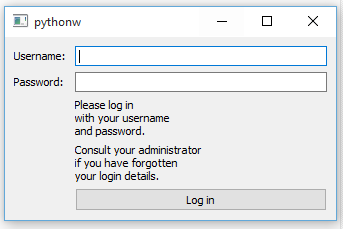
\includegraphics[width=\textwidth]{C:/Users/Jordan/git/COMP4Coursework2/Design/pyqt_figure_1}
\end{figure}

\begin{figure}[H]
    \label{fig:print_function_result}\caption{ErrorMessage2: If the user's input username or password is incorrect, this message will appear.}
    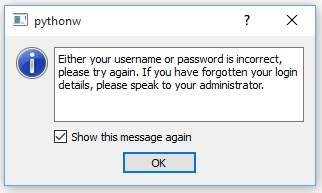
\includegraphics[width=\textwidth]{C:/Users/Jordan/git/COMP4Coursework2/Design/pyqt_figure_2}
\end{figure}

\begin{figure}[H]
    \label{fig:print_function_result}\caption{Student Home Screen: If the user's username is recognised as a student's name, the student version of the home screen will appear.}
    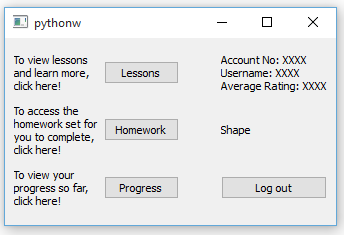
\includegraphics[width=\textwidth]{C:/Users/Jordan/git/COMP4Coursework2/Design/pyqt_figure_3}
\end{figure}

\begin{figure}[H]
    \label{fig:print_function_result}\caption{Lesson Topic Menu: Appears if the user selects the lessons button - displays the topics to choose from.}
    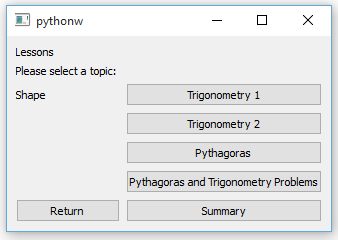
\includegraphics[width=\textwidth]{C:/Users/Jordan/git/COMP4Coursework2/Design/pyqt_figure_4}
\end{figure}

\begin{figure}[H]
    \label{fig:print_function_result}\caption{Lesson Menu: Will appear for any lesson topic selected, displaying the buttons for the topic specific lessons to choose from. Will look the same for each topic except for the button and window names.}
    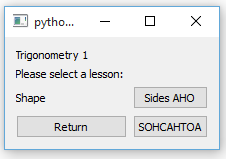
\includegraphics[width=\textwidth]{C:/Users/Jordan/git/COMP4Coursework2/Design/pyqt_figure_5}
\end{figure}

\begin{figure}[H]
    \label{fig:print_function_result}\caption{First Lesson Screen: Will appear with the lessons depending on which button was selected; all lessons will use a generic design plan.}
    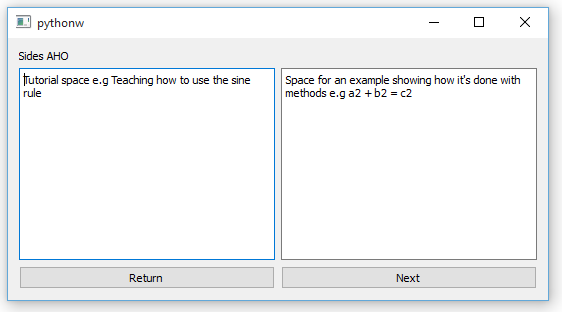
\includegraphics[width=\textwidth]{C:/Users/Jordan/git/COMP4Coursework2/Design/pyqt_figure_6}
\end{figure}

\begin{figure}[H]
    \label{fig:print_function_result}\caption{Second Lesson Screen: Appears once next has been selected from the previous screen, continuing a generic design plan and displaying the next examples.}
    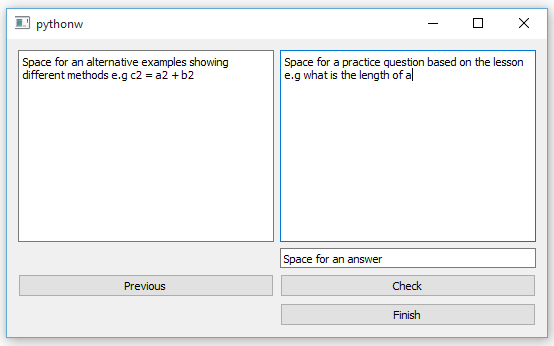
\includegraphics[width=\textwidth]{C:/Users/Jordan/git/COMP4Coursework2/Design/pyqt_figure_7}
\end{figure}

\begin{figure}[H]
    \label{fig:print_function_result}\caption{Homework Topic Menu: Appears if the user selects the homework button - displays the topics to choose from.}
    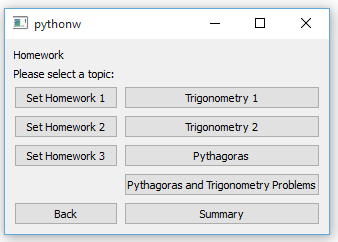
\includegraphics[width=\textwidth]{C:/Users/Jordan/git/COMP4Coursework2/Design/pyqt_figure_8}
\end{figure}

\begin{figure}[H]
    \label{fig:print_function_result}\caption{Homework Menu: Will appear for any homework topic selected, displaying the buttons for the topic specific homeworks to choose from. Will look the same for each topic except for the button and window names.}
    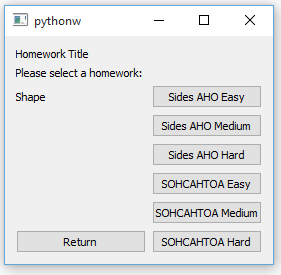
\includegraphics[width=\textwidth]{C:/Users/Jordan/git/COMP4Coursework2/Design/pyqt_figure_9}
\end{figure}

\begin{figure}[H]
    \label{fig:print_function_result}\caption{First Homework Screen: Will appear with the homework depending on which button was selected; all homeworks will use a generic design plan.}
    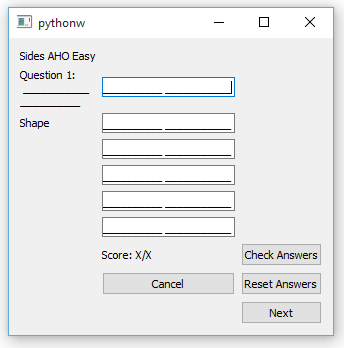
\includegraphics[width=\textwidth]{C:/Users/Jordan/git/COMP4Coursework2/Design/pyqt_figure_10}
\end{figure}

\begin{figure}[H]
    \label{fig:print_function_result}\caption{Second Homework Screen: Appears once next has been selected from the previous screen, continuing a generic design plan and displaying the next questions.}
    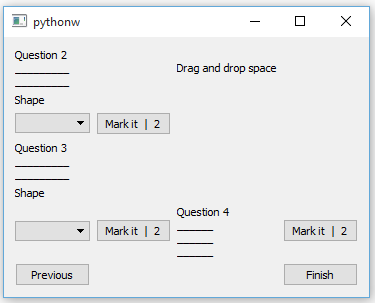
\includegraphics[width=\textwidth]{C:/Users/Jordan/git/COMP4Coursework2/Design/pyqt_figure_11}
\end{figure}

\begin{figure}[H]
    \label{fig:print_function_result}\caption{Individual User Progress Database: Appears if the user selects the progress button - displays their individual database in a table in the window.}
    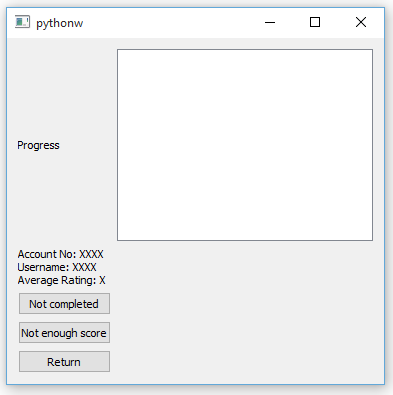
\includegraphics[width=\textwidth]{C:/Users/Jordan/git/COMP4Coursework2/Design/pyqt_figure_12}
\end{figure}

\begin{figure}[H]
    \label{fig:print_function_result}\caption{Administrator Account Home: If the user's username is recognised as an teacher's name, the administrator version of the home screen will appear.}
    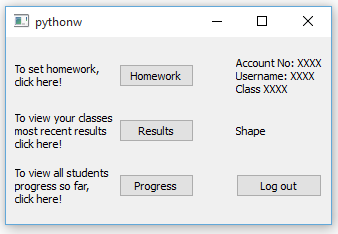
\includegraphics[width=\textwidth]{C:/Users/Jordan/git/COMP4Coursework2/Design/pyqt_figure_13}
\end{figure}

\begin{figure}[H]
    \label{fig:print_function_result}\caption{Homework Setting Topic Menu: Appears if the user selects the homework button - displays the topics to choose from to set as homework.}
    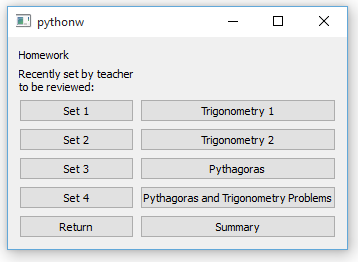
\includegraphics[width=\textwidth]{C:/Users/Jordan/git/COMP4Coursework2/Design/pyqt_figure_14}
\end{figure}

\begin{figure}[H]
    \label{fig:print_function_result}\caption{Homework Set Screen: Appears once a topic has been selected - once the set button is pressed this homework will be available on each student's homework to-do list.}
    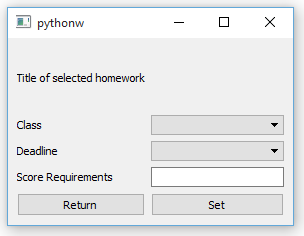
\includegraphics[width=\textwidth]{C:/Users/Jordan/git/COMP4Coursework2/Design/pyqt_figure_15}
\end{figure}

\begin{figure}[H]
    \label{fig:print_function_result}\caption{Results Menu: Appears if the user selects the results button - displays a list of buttons leading to homework recently completed that needs to be checked.}
    \includegraphics[width=\textwidth]{C:/Users/Jordan/git/COMP4Coursework2/Design/pyqt_figure_16}
\end{figure}

\begin{figure}[H]
    \label{fig:print_function_result}\caption{Class Results Database: Once a homework is selected from the previous screen, the database will appear showing all the results for that specific homework.}
    \includegraphics[width=\textwidth]{C:/Users/Jordan/git/COMP4Coursework2/Design/pyqt_figure_17}
\end{figure}

\begin{figure}[H]
    \label{fig:print_function_result}\caption{ErrorMessage3: Appears if the user inputs a wrong data type into an answer box on a homework - should be a decimal.}
    \includegraphics[width=\textwidth]{C:/Users/Jordan/git/COMP4Coursework2/Design/pyqt_figure_18}
\end{figure}

\begin{figure}[H]
    \label{fig:print_function_result}\caption{ErrorMessage3: Appears if the user inputs a wrong data type into an answer box on a homework - should be an intege.r}
    \includegraphics[width=\textwidth]{C:/Users/Jordan/git/COMP4Coursework2/Design/pyqt_figure_19}
\end{figure}

\begin{figure}[H]
    \label{fig:print_function_result}\caption{ErrorMessage3: Appears if the user inputs a wrong data type into an answer box on a homework - should be a string.}
    \includegraphics[width=\textwidth]{C:/Users/Jordan/git/COMP4Coursework2/Design/pyqt_figure_20}
\end{figure}

\begin{figure}[H]
    \label{fig:print_function_result}\caption{ErrorMessage4: Appears if the user gets the wrong answer on an answer box on a homework.}
    \includegraphics[width=\textwidth]{C:/Users/Jordan/git/COMP4Coursework2/Design/pyqt_figure_21}
\end{figure}

\section{Definition of Data Requirements}

\subsection{Identification of all data input items}

\begin{itemize}
	\item Log In Inputs:
	\begin{itemize}
		\item Username
		\item Password
	\end{itemize}
	\item Lesson Inputs:
	\begin{itemize}
		\item Lesson test answer
		\item Check answers button
	\end{itemize}
	\item Homework Set Inputs:
	\begin{itemize}
		\item Class
		\item Deadline
		\item Score Requirements
		\item Set homework button
	\end{itemize}
	\item Homework Inputs:
	\begin{itemize}
		\item Question 1a answer
		\item Question 1b answer
		\item Question 1c answer
		\item Question 1d answer
		\item Question 1e answer
		\item Question 1f answer
		\item Question 2 drop down selection
		\item Question 3 drop down selection
		\item Question 4 drag and drop inputs
		\item Submit answers button
		\item Homework Buttons:
		\begin{itemize}
			\item Reset answers button
			\item Mark answers button
		\end{itemize}
	\end{itemize}
	\item All Other Buttons:
	\begin{itemize}
		\item Log in button
		\item Student Version:
		\begin{itemize}
			\item Lesson button
			\item Homework button
			\item Progress button
			\item Lesson topic buttons	
			\item Lesson buttons
			\item Homework topic buttons
			\item Homework buttons
			\item Set homework buttons
		\end{itemize}
		\item Teacher Version:
		\begin{itemize}
			\item Homework button
			\item Results button
			\item Progress button
			\item Result selection buttons
			\item Feedback
		\end{itemize}
		\item Previous button
		\item Next button
		\item Return button
		\item Finish button
		\item OK button
		\item Log out button
	\end{itemize}
\end{itemize}

\subsection{Identification of all data output items}

\begin{itemize}
	\item Displays:
	\begin{itemize}
		\item All screens
		\item Hard-coded lesson examples
		\item Hard-coded homework questions
		\item Correct answers
	\end{itemize}
	\item Database:
	\begin{itemize}
		\item FirstName
		\item LastName
		\item TaskName
		\item OverallPercentageScore
		\item IndividualPercentageScore (For each question in a homework)
		\item Rating
		\item Feedback (From teacher to student)
	\end{itemize}
	\item Error Messages:
	\begin{itemize}
		\item ErrorMessage2
		\item ErrorMessage3 - Decimal
		\item ErrorMessage3 - Integer
		\item ErrorMessage3 - String
		\item ErrorMessage4
	\end{itemize}
	\item Displayed On Home:
	\begin{itemize}
		\item Account name
		\item Username
		\item Average rating (Student)
		\item Class (Teacher)
	\end{itemize}
\end{itemize}

\subsection{Explanation of how data output items are generated}

\begin{center}
\begin{tabular}{|p{4cm}|p{6cm}|} \hline
\textbf{Output} & \textbf{How it's generated} \\ \hline
Lesson Examples & These are hard-coded and will be saved as overrides in each lesson's subclass \\ \hline
Homework Examples & These are hard-coded and will be saved as overrides in each homework's subclass \\ \hline
Correct Answers & These will be generated using algorithms which will solve the same problem the user is trying to solve, find the answer, and display it \\ \hline
FirstName & This will be saved to the database once the administrator inputs the class names \\ \hline
LastName & This will be saved to the database once the administrator inputs the class names \\ \hline
TaskName & This will be hard-coded as an attribute in each subclass \\ \hline
OverallPercentageScore & When a homework task is submitted, algorithms will check how many answers were correct, and obtain a percentage from them, then calculate the average from them \\ \hline
IndividualPercentageScore & When a homework task is submitted, algorithms will check how many answers were correct, and obtain a percentage from each question from the average of each question's parts \\ \hline
Rating & This will be decided using selection statements depending on what the OverallPercentageScore is \\ \hline
Feedback & The administrator will manually input this and the user will then be able to see it on their individual results page \\ \hline
ErrorMessage2 & This is a hard-coded QErrorMessage() which will appear if the user inputs an incorrect username or password \\ \hline
ErrorMessage3 & These are hard-coded QErrorMessage()s which will appear if the user inputs an incorrect data type as an answer, depending on what the data type is supposed to be \\ \hline
\end{tabular}
\end{center}

\begin{center}
\begin{tabular}{|p{4cm}|p{6cm}|}  \hline
\textbf{Output} & \textbf{How it's generated} \\ \hline
ErrorMessage4 & This is a hard-coded QErrorMessage() which will appear if the user inputs an incorrect answer to a  homework question \\ \hline
Account Name & Will be a unique identifier saved by the system, only visible on the homescreens \\ \hline
Username & This is the same as the username used to log in, and will be obtained from the same place it's saved for validation, probably a notepad file \\ \hline
Average Rating & All of the user's past homework's ratings will be averaged and displayed on the homescreen \\ \hline
Class & This will be input by the administrator before inputting each students name \\ \hline
\end{tabular}
\end{center}

\subsection{Data Dictionary}

\begin{center}
\begin{tabular}{|p{3.4cm}|p{1.2cm}|p{2cm}|p{2cm}|p{2cm}|p{3.5cm}|}
\hline
\textbf{Name} & \textbf{Data Type} & \textbf{Length} & \textbf{Validation} & \textbf{Example Data} & \textbf{Comment} \\ \hline
UserID & Integer & 4 bits & 0001 to 9999 & 1546 & Unique to each user \\ \hline
Password & String and integers & 7 characters & letter followed by number followed by letter & f7h3j5f & The password generator uses mixed data types to avoid inappropriate passwords \\ \hline
FirstName & String & 15 characters & First letter upper case, rest lower case & John & Unique to each user, but could be shared by some \\ \hline
Surname & String & 25 characters & First letter upper case, rest lower case & Smith & Unique to each user, but could be shared by some \\ \hline
TaskName & String & 25 characters & & Trigonometry 2 & Hard-coded into the system \\ \hline
OverallPercentScore & Real & 3 characters & in range 0 - 100 & 76.5\% & The percentage of marks obtained in a test, decimal points allowed \\ \hline
\end{tabular}
\end{center}

\begin{center}
\begin{tabular}{|p{3.4cm}|p{1.2cm}|p{2cm}|p{2cm}|p{2cm}|p{3.5cm}|}
\hline
\textbf{Name} & \textbf{Data Type} & \textbf{Length} & \textbf{Validation} & \textbf{Example Data} & \textbf{Comment} \\ \hline
IndividualPercentScore & Real & 3 characters & in range 0 - 100 & 45.5\% & The percentage of marks for an individual question, field will only appear in separate table for individual tasks \\ \hline
Rating & Blob & 64 kilobytes & \ &  Green face graphic & Green, amber or red face graphic \\ \hline
Feedback & String & 500 characters & \ & Good work & This can consist of any characters as it is a personal message \\ \hline
AppointmentTime & Time & 5 characters & 24 hour format & 13:35 & Only relevant if the user has a true SeeAfterClass variable, set automatically bsed on the administrator's timetable but can be changed if necessary\\ \hline
SeeAfterClass & Boolean & 3 characters & Yes or No & Yes & If the user doesn't achieve a sufficient score, this variable will become true and alert the user \\ \hline
ErrorMessage1 & String & 50 characters & & Sorry, the name cannot have integers & An error message if the wrong data type is used to input a name \\ \hline
ErrorMessage2 & String & 50 characters & & Sorry, that is not a valid login & Tells the user if they have input the wrong username or password \\ \hline
ErrorMessage3 & String & 50 characters & & Please input a decimal, not an integer & Tells the user if their incorrect answer is the wrong data type \\ \hline
ErrorMessage4 & String & 50 characters & & That is incorrect, try one more time & Tells the user that their answer is incorrect and gives them one more attempt \\ \hline
CorrectAnswer & Integer, Real, String & 5 characters & Must be a decimal or whole number, or text & 25.5cm & Gives the user the correct answer if they get the question wrong too many times \\ \hline
\end{tabular}
\end{center}

\begin{center}
\begin{tabular}{|p{3.4cm}|p{1.2cm}|p{2cm}|p{2cm}|p{2cm}|p{3.5cm}|}
\hline
\textbf{Name} & \textbf{Data Type} & \textbf{Length} & \textbf{Validation} & \textbf{Example Data} & \textbf{Comment} \\ \hline
Login data & String & 25 characters & & johnsmith1, f8j4h6k & The login information saved in the system to be loaded and checked with the user's inputs \\ \hline
Task data & String & 100 characters & & Trigonometry - sin rule, Level 7, Trigonometry & Contains all the information about the task, what difficulty it is, what type it is etc. \\ \hline
Set answers & Integer, Real, String & 5 characters & Must be a decimal or whole number, or text if in a text box & 45{$^o$} & Contains all the set answers for some of the tasks \\ \hline
Calculated answers & Integer, Real & 5 characters & Must be the same solution as the algorithm & 29.8 & Contains algorithms which find and validate the solution for randomly generated tasks \\ \hline
Account name & Integer & 4 characters & Must be a string of 4 integers, 0 - 9 & 1357 & This is the unique identifier for the database \\ \hline
Average rating & Blob & 1 blob & Will be a green, amber or red face & Green face blob & This is the rating from the average rating of each student's completed homework so far \\ \hline
Class & String & 3 - 6 characters & Must be the name of the class, same as is in the centre's system & 10A & Is input with the student names \\ \hline
\end{tabular}
\end{center}

\subsection{Identification of appropriate storage media}

My system files will need to be stored on the school's local server, as every part will need to be accessible from every computer, to save the teacher having to log into every computer one at a time to check work. this way, every computer can access every account, and if they have the permissions, every part of the database. If necessary, some files can be backed up onto an individual computer in the system, or onto a USB stick. As a result, all users and administrators will be able to share the files and use them at the same time.

\section{Database Design}

\subsection{Normalisation}

\subsubsection{ER Diagrams}

\begin{figure}[H]
    \label{fig:print_function_result}
    \includegraphics[width=\textwidth]{C:/Users/Jordan/git/COMP4Coursework2/Design/er_diagram}
\end{figure}

\subsubsection{Entity Descriptions}

\begin{center}
\begin{tabular}{|p{3cm}|p{4cm}|p{4cm}|p{3cm}|} \hline
\textbf{Entity} & \textbf{Description} & \textbf{Attributes} & \textbf{Key} \\ \hline
Student & Each record shows how many results a student receives, and which class they are in & \textbf{Student}(\underline{StudentID}, \underline{ClassID}) & Primary Key(StudentID, ClassID) \\ \hline
Class & Shows which students are in the class and the teacher of that class, and how much homework the class has been set & \textbf{Class}(\underline{ClassID}, TeacherID) & Primary Key(ClassID) \\ \hline
Homework & Shows who each homework has been set for, and the results if the homework has been completed & \textbf{Homework}(\underline{HomeworkID}, HomeworkSet, HomeworkResults) & Primary Key(HomeworkID) \\ \hline 
HomeworkSet & Shows who has been set the homework, when, and how many times/how long for & \textbf{HomeworkSet}(\underline{ClassID}, \underline{HomeworkID}, DueDate, SetDate) & Primary Key(ClassID, HomeworkID) \\ \hline
HomeworkResults & This record contains all of the results for a completed homework & \textbf{HomeworkResults} (\underline{HomeworkID}, \underline{StudentID}, \underline{QuestionID}, Rating, CompletedDate) & Primary Key(HomeworkID, StudentID, QuestionID) \\ \hline
Question & Shows how many questions were in a homework, and the percentage which are correct in each students results & \textbf{Question}(\underline{HomeworkID}, \underline{QuestionID}, QuestionText, Choice1, Choice2, ChoiceX, CorrectAnswer, TypeOfQuestion) & Primary Key(HomeworkID, QuestionID) \\ \hline
\end{tabular}
\end{center}

\subsubsection{UNF to 3NF}

\textbf{Unnormalised: }

\begin{center}
\begin{tabular}{|p{4cm}|} \hline
AccountID \\
UserID \\
ClassID
FirstName \\
LastName \\
TaskName \\
OverallPercentScore \\
IndividualPercentScore \\
Rating \\
Feedback \\ \hline
\end{tabular}
\end{center}

\textbf{1st Normalised Form: }

\begin{center}
\begin{tabular}{|p{4cm}|p{3cm}|} \hline
\textbf{Repeating Attributes} & \textbf{Non-repeating Attributes} \\ \hline
\textbf{\underline{UserID}} & \textbf{\underline{AccountID}} \\
\textbf{\underline{ClassID}} & \\
\textbf{\underline{TaskName}} & \\
FirstName & \\
LastName & \\
OverallPercentScore & \\
IndividualPercentScore & \\
Feedback & \\
Rating & \\ \hline
\end{tabular}
\end{center}

\textbf{2nd Normalised Form: }

\begin{center}
\begin{tabular}{|p{4cm}|p{3cm}|} \hline
\textbf{Repeating Attributes} & \textbf{Non-repeating Attributes} \\ \hline
\textbf{\underline{ClassID}} & \textbf{\underline{AccountID}} \\
\textbf{\underline{UserID}} & \\
FirstName & \\
LastName & \\
 & \\
\textbf{\underline{TaskName}} & \\
OverallPercentScore & \\
IndividualPercentScore & \\
Feedback & \\
Rating & \\ \hline
\end{tabular}
\end{center}

\textbf{3rd Normalised Form: }

\begin{center}
\begin{tabular}{|p{4cm}|p{3cm}|} \hline
\textbf{Repeating Attributes} & \textbf{Non-repeating Attributes} \\ \hline
\textbf{\underline{ClassID}} & \textbf{\underline{AccountID}} \\
\textbf{\underline{UserID}} & \\
FirstName & \\
LastName & \\
 & \\
\textbf{\underline{TaskName}} & \\
\underline{IndividualPercentScore} & \\
& \\
\textbf{\underline{IndividualPercentScore}} & \\
\underline{OverallPercentScore} & \\
& \\
\textbf{\underline{OverallPercentScore}} & \\
Rating & \\
Feedback & \\ \hline
\end{tabular}
\end{center}

\subsection{SQL Queries}

\begin{center}
\begin{tabular}{|p{8cm}|p{6cm}|} \hline
\textbf{SQL Query (Python Format)} & \textbf{Description} \\ \hline
sql = """create table Student & This is the SQL statement which \\ 
(UserID integer, & creates the initial table called \\
FirstName text, & Student, with all of the attributes \\
LastName text, & that need to be displayed to the users \\
TaskName text, & in the database \\
OverallPercentScore real, & \\
IndividualPercentScore real, &\\
Rating blob, & \\
Feedback text, & \\
primary key(UserID))""" & \\ \hline
"""insert into Student & This query adds values to the \\
(FirstName, LastName, UserID) values ('\{0\}', '\{1\}', '\{2\}') & FirstName, LastName and UserID \\
""".format(FirstName, LastName, UserID) & fields when the administrator adds names to the system \\ \hline
"""select * from Student & This query is for student use and it \\
where TaskName = '\{0\}' and UserID = '\{1\}' & fetches all of the database information \\
""".format(TaskName, UserID) & for that user for a specific homework they have completed \\ \hline
"""select * from Class & This query is for teacher use and it \\
where TaskName = '\{0\}' and ClassID = '\{1\}' & fetches all of the records saved for an\\
""".format(TaskName, ClassID) & entire class for a specific homework \\ \hline
"""select * from Class & This query will fetch all of the records \\
where StudentID = '\{0\}'""".format(StudentID) & stored for a specific student, for teacher use \\ \hline
"""select * from Class & This query can be used by the teacher \\
where TaskName = '\{0\}' and Rating = '\{1\}' & to search for all homework done in a \\
""".format(TaskName, Rating) & class which has not been done to a sufficient standard \\ \hline
"""select * from Student & This query will select all of the \\
where StudentID = '\{0\}' and Rating = '\{1\}' & homework done by one student which \\
""".format(StudentID, Rating) & has not been done to a sufficient standard \\ \hline
"""update Student & This query will update the database \\
OverallPercentScore = '\{0\}' & with the results when a student \\
IndividualPercentScore = '\{1\}' & completes a homework \\
Rating = '\{2\}' & \\
where StudentID = '\{3\}' and TaskName = '\{4\}' & \\
""".format(OverallPercentScore, IndividualPercentScore, Rating, StudentID, TaskName) & \\ \hline
\end{tabular}
\end{center}

\begin{center}
\begin{tabular}{|p{8cm}|p{6cm}|} \hline
\textbf{SQL Query (Python Format)} & \textbf{Description} \\ \hline
"""update Student & This query will update the records \\
Feedback = '\{0\}' & for a student when the \\
where StudentID = '\{1\}' and TaskName = '\{2\}' & teacher manually gives them \\
""".format(Feedback, StudentID, TaskName) & feedback \\ \hline
\end{tabular}
\end{center}

\section{Security and Integrity of the System and Data}

\subsection{Security and Integrity of Data}

As this system will store a small amount of personal data (FirstName, LastName, ClassID), the Data Protection Act of 1998 must be followed. Therefore the data must be kept up to date, and a way of editing the FirstName, LastName and ClassID records will be included to ensure that wrong data is not forced to be kept permanently, should it be input by mistake. To ensure that the data is not kept for longer than the DPA says it should be, any old data will be searched for and deleted whenever the system is started, should it be found. Furthermore, checks shall be implemented to ensure key data fields are not left empty, in order to maintain referential integrity. The only possible way to view the data stored by my system will be on the visual database in the graphical user interface, which will only be accessible following the input of a correct username and password. Finally, all of the data stored will be valid and feasible as drop down menus, and data type relevant error messages will be used to ensure the user is given a fair chance to input answers.

\subsection{System Security}

In order to prevent theft of information and tampering, all information in the system will only be accessible by providing a username and password, and each user will only be allowed to view data relevant to their own progression. Students will not be able to change any information in the database, but teachers will, if they accidentally include a typo when inputting names into the system. Furthermore, the number of people with access to the system will be limited, and those with key access trusted as professional teachers. The database will be encrypted to avoid people somehow accessing the database information by some other means, although only names will be stored as personal information. Lastly, all of the names input into the system will have a validation check to ensure they do not accidentally include numbers, extra capital letters, not enough capital letters or other characters not in the alphabet. Because the names stored will fall under the Data Protection Act, I will ensure that no data is sent to other countries, or even anywhere at all outside of the school, that the data is secure and only accessible by authorised people, that it is only stored by the school, that the data can be updated and destroyed to ensure protection, and that only necessary data will be collected in the first place.

\section{Validation}

\begin{center}
\begin{tabular}{|p{2cm}|p{3cm}|p{4cm}|p{4cm}|} \hline
\textbf{Item} & \textbf{Example} & \textbf{Validation applied} & \textbf{Comments} \\ \hline
ClassID & 10A & Presence check & The ClassID is the same as the classes actual class name, so no validation is required \\ \hline
FirstName & John & Data type check: First letter, capital, rest lower case, all string, no spaces & Checks that the name given is in fact a name \\ \hline
LastName & Smith & Data type check: First letter, capital, rest lower case, all string, no spaces & Checks that the name given is in fact a name \\ \hline
Username & User \ 1 & Format check: First 4 letters of LastName followed by a number. Validation check - Check it's in the system as a valid username & This ensures that the username is in the right format before checking if it's recognised as a valid username \\ \hline
Password & f5h3d7h & Format check: letter, number, letter, number, letter, number, letter, all lower case. Validation check - Check it's in the system and matches the username input beforehand & The password is randomly generated and attached to the username, in that format to avoid any inappropriate words being generated \\ \hline
Text answer input & 7 & ValueErrorCheck - integer & Checks that the value input is the correct data type \\ \hline
Text answer input & 7.5 & ValueErrorCheck - decimal & Checks that the value input is the correct data type \\ \hline
Text answer input & seven & ValueErrorCheck - string & Checks that the value input is the correct data type  \\ \hline
ComboBox answer input & select 5 & Presence check & Checks that an option has actually been selected \\ \hline
Drag and drop answer input & all pictures dropped onto shape & Presence check & Checks to see if all of the drag icons have been dropped into the corresponding spaces \\ \hline
Correct & True & Presence check & This boolean corresponds to every answer and says whether or not it is correct \\ \hline
\end{tabular}
\end{center}

\begin{center}
\begin{tabular}{|p{2cm}|p{3cm}|p{4cm}|p{4cm}|} \hline
\textbf{Item} & \textbf{Example} & \textbf{Validation applied} & \textbf{Comments} \\ \hline
Class selected & 10A and & Presence check & Makes sure a class has been selected from the combo box to set the homework for \\ \hline
Deadline & 14/12/15 & Presence check & Makes sure a date within a given set of boundaries has been selected from the combo box \\ \hline
Score Requirements & 75\% & Presence check & Makes sure a score percentage has been selected from the combo box \\ \hline
\end{tabular}
\end{center}

\section{Testing}

\begin{landscape}
\subsection{Outline Plan}

\begin{center}
    \begin{tabular}{|p{2cm}|p{5cm}|p{5cm}|p{4cm}|}
        \hline
        \textbf{Test Series} & \textbf{Purpose of Test Series} & \textbf{Testing Strategy} & \textbf{Strategy Rationale}\\ \hline
        1 & Test the connections between all of the buttons on the user interfaces & Top-down testing & Each button will be tested to make sure it connects to the right screen \\ \hline
        2 & Test all of the input spaces & Bottom-up testing & Each input will be tested once it is developed \\ \hline
        3 & Test all information is stored in the correct place in the database & Black box testing & The database will be viewed in a database viewer to ensure that SQL queries are working and data is being stored in the database once they have been developed \\ \hline
	4 & Test all of the algorithms to make sure that the program gives the correct output and marks, both mathematical or other & White box testing & Each algorithm will be tested once it is developed \\ \hline
	5 & Test that the system fulfils the clients request & Acceptance testing & The system will be developed once it is completed to a usable standard \\ \hline
    \end{tabular}
\end{center}

\subsection{Detailed Plan}

\begin{center}
    \begin{longtable}{|p{1.5cm}|p{2.5cm}|p{2.5cm}|p{2cm}|p{2cm}|p{2cm}|p{2cm}|p{2cm}|}
        \hline
        \textbf{Test Series} & \textbf{Purpose of Test} & \textbf{Test Description} & \textbf{Test Data} & \textbf{Test Data Type (Normal/ Erroneous/ Boundary)} & \textbf{Expected Result} & \textbf{Actual Result} & \textbf{Evidence}\\ \hline
1.001 & To test the student log in button on the first menu functions as intended & This should link to the student menu screen & Click the log in button & Normal & The student account screen should be displayed & & \\ \hline
1.002 & To test the teacher log in button on the first menu functions as intended & This should link to the administrator menu screen & Click the log in button & Normal & The administrator account screen should be displayed & & \\ \hline
1.003 & To test the lessons button on the student account screen functions as intended & This should link to the lesson topic menu screen & Click the lessons button & Normal & The lesson topic menu should be displayed & & \\ \hline
1.004 & To test the homework button on the student account screen functions as intended & This should link to the homework topic menu screen & Click the homework button & Normal & The homework topic menu should be displayed & & \\ \hline
1.005 & To test the progress button on the student account screen functions as intended & This should link to the student's personal database display screen & Click the progress button & Normal & The student's personal database screen should be displayed & & \\ \hline
1.006 & To test the log out button on the student account screen functions as intended & This should close down the entire program & Click the log out button & Normal & The program should stop & & \\ \hline
1.007 & To test the Trigonometry 1 button on the lesson topic menu screen functions as intended & This should link to the trigonometry 1 menu screen & Click the Trigonometry 1 button & Normal & The topic's menu screen should be displayed & & \\ \hline
1.008 & To test the Trigonometry 2 button on the lesson topic menu screen functions as intended & This should link to the trigonometry 2 menu screen & Click the Trigonometry 2 button & Normal & The topic's menu screen should be displayed & & \\ \hline
1.009 & To test the Pythagoras button on the lesson topic menu screen functions as intended & This should link to the pythagoras menu screen & Click the Pythagoras button & Normal & The topic's menu screen should be displayed & & \\ \hline
1.010 & To test the Pythagoras and Trigonometry Problems button on the lesson topic menu screen functions as intended & This should link to the trigonometry and pythagoras problems menu screen & Click the Pythaogras and Trigonometry Problems button & Normal & The topic's menu screen should be displayed & & \\ \hline
1.011 & To test the Summary button on the lesson topic menu screen functions as intended & This should link to the summary menu screen & Click the Summary button & Normal & The topic's menu screen should be displayed & & \\ \hline
1.012 & To test the return button on the lesson topic menu functions as intended & This should link back to the student account screen & Click the return button & Normal & The student account screen should be displayed & & \\ \hline
1.013 & To test the Sides button on the Trigonometry 1 lesson menu functions as intended & This should link to the screen for the first page of the sides lesson & Click the Sides button & Normal & The first sides lesson screen should be displayed & & \\ \hline
1.014 & To test the SOHCAHTOA button on the Trigonometry 1 lesson menu functions as intended & This should link to the screen for the first page of the SOHCAHTOA lesson & Click the SOHCAHTOA button & Normal & The first SOHCAHTOA lesson screen should be displayed & & \\ \hline
1.015 & To test the return button on the Trigonometry 1 menu functions as intended & This should link back to the lesson topic menu screen & Click the return button & Normal & The lesson topic menu should be displayed & & \\ \hline
1.016 & To test the Finding Angles button on the Trigonometry 2 lesson menu functions as intended & This should link to the screen for the first page of the finding angles lesson & Click the Finding angles button & Normal & The first finding angles lesson screen should be displayed & & \\ \hline
1.017 & To test the Inverted Angles button on the Trigonometry 2 lesson menu functions as intended & This should link to the screen for the first page of the inverted angles lesson & Click the Inverted angles button & Normal & The first inverted angles lesson screen should be displayed & & \\ \hline
1.018 & To test the 3D Trigonometry button on the Trigonometry 2 lesson menu functions as intended & This should link to the screen for the first page of the 3D Trigonometry lesson & Click the 3D Trigonometry button & Normal & The first 3D trigonometry lesson screen should be displayed & & \\ \hline
1.019 & To test the return button on the Trigonometry 2 menu functions as intended & This should link back to the lesson topic menu screen & Click the return button & Normal & The lesson topic menu should be displayed & & \\ \hline
1.020 & To test the Pythagoras Theorem button on the Pythagoras lesson menu functions as intended & This should link to the screen for the first page of the pythagoras theorem lesson & Click the pythagoras theorem button & Normal & The first pythagoras theorem lesson screen should be displayed & & \\ \hline
1.021 & To test the 3D Pythagoras button on the Pythagoras lesson menu functions as intended & This should link to the screen for the first page of the 3D pythagoras lesson & Click the 3D pythagoras button & Normal & The first 3D pythagoras lesson screen should be displayed & & \\ \hline
1.022 & To test the return button on the Pythagoras menu functions as intended & This should link back to the lesson topic menu screen & Click the return button & Normal & The lesson topic menu should be displayed & & \\ \hline
1.023 & To test the Easy Pythagoras and Trigonometry Problems button on the Trigonometry and Pythagoras Problems lesson menu functions as intended & This should link to the screen for the first page of the easy pythagoras and trigonometry problems lesson & Click the easy pythagoras and trigonometry problems button & Normal & The first easy pythagoras and trigonometry problems lesson screen should be displayed & & \\ \hline
1.024 & To test the Medium Pythagoras and Trigonometry Problems button on the Trigonometry and Pythagoras Problems lesson menu functions as intended & This should link to the screen for the first page of the medium pythagoras and trigonometry problems lesson & Click the medium pythagoras and trigonometry problems button & Normal & The first medium pythagoras and trigonometry problems lesson screen should be displayed & & \\ \hline
1.025 & To test the Hard Pythagoras and Trigonometry Problems button on the Trigonometry and Pythagoras Problems lesson menu functions as intended & This should link to the screen for the first page of the hard pythagoras and trigonometry problems lesson & Click the hard pythagoras and trigonometry problems button & Normal & The first hard pythagoras and trigonometry problems lesson screen should be displayed & & \\ \hline
1.026 & To test the return button on the Pythagoras and Trigonometry Problems menu functions as intended & This should link back to the lesson topic menu screen & Click the return button & Normal & The lesson topic menu should be displayed & & \\ \hline
1.027 & To test the Revise Trigonometry 1 button on the Summary lesson menu functions as intended & This should link to the screen for the first page of the revise trigonometry 1 lesson & Click the revise trigonometry 1 button & Normal & The first revise trigonometry 1 lesson screen should be displayed & & \\ \hline
1.028 & To test the Revise Trigonometry 2 button on the Summary lesson menu functions as intended & This should link to the screen for the first page of the revise trigonometry 2 lesson & Click the revise trigonometry 2 button & Normal & The first revise trigonometry 2 lesson screen should be displayed & & \\ \hline
1.029 & To test the Revise Trigonometry 3 button on the Summary lesson menu functions as intended & This should link to the screen for the first page of the revise trigonometry 3 lesson & Click the revise trigonometry 3 button & Normal & The first revise trigonometry 3 lesson screen should be displayed & & \\ \hline
1.030 & To test the return button on the Summary menu functions as intended & This should link back to the lesson topic menu screen & Click the return button & Normal & The lesson topic menu should be displayed & & \\ \hline
1.031 & To test the return button on the first Sides lesson screen functions as intended & This should link back to the Trigonometry 1 menu screen & Click the Sides return button & Normal & The Trigonometry 1 menu screen should be displayed & & \\ \hline
1.032 & To test the next button on the first Sides lesson screen functions as intended & This should link to the second Sides lesson screen & Click the Sides next button & Normal & The second Sides lesson screen should be displayed & & \\ \hline
1.033 & To test the previous button on the second Sides lesson screen functions as intended & This should link back to the first Sides lesson screen & Click the Sides previous button & Normal & The first Sides lesson screen should be displayed & & \\ \hline
1.034 & To test the Check Answer button on the second Sides lesson screen functions as intended & This should run an algorithm to check if the user's input is correct or not, and tell them & Click the Sides check answers button & Normal & A truthful 'Correct' or 'Incorrect' message should be displayed & & \\ \hline
1.035 & To test the Finish button on the second Sides lesson screen functions as intended & This close the lesson and return to the lesson topic menu screen & Click the Sides finish button & Normal & The Lesson Topic Menu screen should be displayed & & \\ \hline
1.036 & To test the return button on the first SOHCAHTOA lesson screen functions as intended & This should link back to the Trigonometry 1 menu screen & Click the SOHCAHTOA return button & Normal & The Trigonometry 1 menu screen should be displayed & & \\ \hline
1.037 & To test the next button on the first SOHCAHTOA lesson screen functions as intended & This should link to the second SOHCAHTOA lesson screen & Click the SOHCAHTOA next button & Normal & The second SOHCAHTOA lesson screen should be displayed & & \\ \hline
1.038 & To test the previous button on the second SOHCAHTOA lesson screen functions as intended & This should link back to the first SOHCAHTOA lesson screen & Click the SOHCAHTOA previous button & Normal & The first SOHCAHTOA lesson screen should be displayed & & \\ \hline
1.039 & To test the Check Answer button on the second SOHCAHTOA lesson screen functions as intended & This should run an algorithm to check if the user's input is correct or not, and tell them & Click the SOHCAHTOA check answers button & Normal & A truthful 'Correct' or 'Incorrect' message should be displayed & & \\ \hline
1.040 & To test the Finish button on the second SOHCAHTOA lesson screen functions as intended & This should close the lesson and return to the lesson topic menu screen & Click the SOHCAHTOA finish button & Normal & The Lesson Topic Menu screen should be displayed & & \\ \hline
1.041 & To test the return button on the first Finding Angles lesson screen functions as intended & This should link back to the Trigonometry 2 menu screen & Click the Finding Angles return button & Normal & The Trigonometry 2 menu screen should be displayed & & \\ \hline
1.042 & To test the next button on the first Finding Angles lesson screen functions as intended & This should link to the second Finding Angles lesson screen & Click the Finding Angles next button & Normal & The second Finding Angles lesson screen should be displayed & & \\ \hline
1.043 & To test the previous button on the second Finding Angles lesson screen functions as intended & This should link back to the first Finding Angles lesson screen & Click the Finding Angles previous button & Normal & The first Finding Angles lesson screen should be displayed & & \\ \hline
1.044 & To test the Check Answer button on the second Finding Angles lesson screen functions as intended & This should run an algorithm to check if the user's input is correct or not, and tell them & Click the Finding Angles check answers button & Normal & A truthful 'Correct' or 'Incorrect' message should be displayed & & \\ \hline
1.045 & To test the Finish button on the second Finding Angles lesson screen functions as intended & This should close the lesson and return to the lesson topic menu screen & Click the Finding Angles finish button & Normal & The Lesson Topic Menu screen should be displayed & & \\ \hline
1.046 & To test the return button on the first Inverted Angles lesson screen functions as intended & This should link back to the Trigonometry 2 menu screen & Click the Inverted Angles return button & Normal & The Trigonometry 2 menu screen should be displayed & & \\ \hline
1.047 & To test the next button on the first Inverted Angles lesson screen functions as intended & This should link to the second Inverted Angles lesson screen & Click the Inverted Angles next button & Normal & The second Inverted Angles lesson screen should be displayed & & \\ \hline
1.048 & To test the previous button on the second Inverted Angles lesson screen functions as intended & This should link back to the first Inverted Angles lesson screen & Click the Inverted Angles previous button & Normal & The first Inverted Angles lesson screen should be displayed & & \\ \hline
1.049 & To test the Check Answer button on the second Inverted Angles lesson screen functions as intended & This should run an algorithm to check if the user's input is correct or not, and tell them & Click the Inverted Angles check answers button & Normal & A truthful 'Correct' or 'Incorrect' message should be displayed & & \\ \hline
1.050 & To test the Finish button on the second Inverted Angles lesson screen functions as intended & This should close the lesson and return to the lesson topic menu screen & Click the Inverted Angles finish button & Normal & The Lesson Topic Menu screen should be displayed & & \\ \hline
1.051 & To test the return button on the first 3D Trigonometry lesson screen functions as intended & This should link back to the Trigonometry 2 menu screen & Click the 3D Trigonometry return button & Normal & The Trigonometry 2 menu screen should be displayed & & \\ \hline
1.052 & To test the next button on the first 3D Trigonometry lesson screen functions as intended & This should link to the second 3D Trigonometry lesson screen & Click the 3D Trigonometry next button & Normal & The second 3D Trigonometry lesson screen should be displayed & & \\ \hline
1.053 & To test the previous button on the second 3D Trigonometry lesson screen functions as intended & This should link back to the first 3D Trigonometry lesson screen & Click the 3D Trigonometry previous button & Normal & The first 3D Trigonometry lesson screen should be displayed & & \\ \hline
1.054 & To test the Check Answer button on the second 3D Trigonometry lesson screen functions as intended & This should run an algorithm to check if the user's input is correct or not, and tell them & Click the 3D Trigonometry check answers button & Normal & A truthful 'Correct' or 'Incorrect' message should be displayed & & \\ \hline
1.055 & To test the Finish button on the second 3D Trigonometry lesson screen functions as intended & This should close the lesson and return to the lesson topic menu screen & Click the 3D Trigonometry finish button & Normal & The Lesson Topic Menu screen should be displayed & & \\ \hline
1.056 & To test the return button on the first Pythagoras Theorem lesson screen functions as intended & This should link back to the Pythagoras menu screen & Click the Pythagoras Theorem return button & Normal & The Pythagoras menu screen should be displayed & & \\ \hline
1.057 & To test the next button on the first Pythagoras Theorem lesson screen functions as intended & This should link to the second Pythagoras Theorem lesson screen & Click the Pythagoras Theorem next button & Normal & The second Pythagoras Theorem lesson screen should be displayed & & \\ \hline
1.058 & To test the previous button on the second Pythagoras Theorem lesson screen functions as intended & This should link back to the first Pythagoras Theorem lesson screen & Click the Pythagoras Theorem previous button & Normal & The first Pythagoras Theorem lesson screen should be displayed & & \\ \hline
1.059 & To test the Check Answer button on the second Pythagoras Theorem lesson screen functions as intended & This should run an algorithm to check if the user's input is correct or not, and tell them & Click the Pythagoras Theorem check answers button & Normal & A truthful 'Correct' or 'Incorrect' message should be displayed & & \\ \hline
1.060 & To test the Finish button on the second Pythagoras Theorem lesson screen functions as intended & This should close the lesson and return to the lesson topic menu screen & Click the Pythagoras Theorem finish button & Normal & The Lesson Topic Menu screen should be displayed & & \\ \hline
1.061 & To test the return button on the first 3D Pythagoras lesson screen functions as intended & This should link back to the Pythagoras menu screen & Click the 3D Pythagoras return button & Normal & The Pythagoras menu screen should be displayed & & \\ \hline
1.062 & To test the next button on the first 3D Pythagoras lesson screen functions as intended & This should link to the second 3D Pythagoras lesson screen & Click the 3D Pythagoras next button & Normal & The second 3D Pythagoras lesson screen should be displayed & & \\ \hline
1.063 & To test the previous button on the second 3D Pythagoras lesson screen functions as intended & This should link back to the first 3D Pythagoras lesson screen & Click the 3D Pythagoras previous button & Normal & The first 3D Pythagoras lesson screen should be displayed & & \\ \hline
1.064 & To test the Check Answer button on the second 3D Pythagoras lesson screen functions as intended & This should run an algorithm to check if the user's input is correct or not, and tell them & Click the 3D Pythagoras check answers button & Normal & A truthful 'Correct' or 'Incorrect' message should be displayed & & \\ \hline
1.065 & To test the Finish button on the second 3D Pythagoras lesson screen functions as intended & This should close the lesson and return to the lesson topic menu screen & Click the 3D Pythagoras finish button & Normal & The Lesson Topic Menu screen should be displayed & & \\ \hline
1.066 & To test the return button on the first Pythagoras and Trigonometry Problems Easy lesson screen functions as intended & This should link back to the Pythagoras and Trigonometry Problems menu screen & Click the Pythagoras and Trigonometry Easy return button & Normal & The Pythagoras and Trigonometry Problems menu screen should be displayed & & \\ \hline
1.067 & To test the next button on the first Pythagoras and Trigonometry Problems Easy lesson screen functions as intended & This should link to the second Pythagoras and Trigonometry Problems Easy lesson screen & Click the Pythagoras and Trigonometry Problems Easy next button & Normal & The second Pythagoras and Trigonometry Problems Easy lesson screen should be displayed & & \\ \hline
1.068 & To test the previous button on the second Pythagoras and Trigonometry Problems Easy lesson screen functions as intended & This should link back to the first Pythagoras and Trigonometry Problems Easy lesson screen & Click the Pythagoras and Trigonometry Problems Easy previous button & Normal & The first Pythagoras and Trigonometry Problems Easy lesson screen should be displayed & & \\ \hline
1.069 & To test the Check Answer button on the second Pythagoras and Trigonometry Problems Easy lesson screen functions as intended & This should run an algorithm to check if the user's input is correct or not, and tell them & Click the Pythagoras and Trigonometry Problems Easy check answers button & Normal & A truthful 'Correct' or 'Incorrect' message should be displayed & & \\ \hline
1.070 & To test the Finish button on the second Pythagoras and Trigonometry Problems Easy lesson screen functions as intended & This should close the lesson and return to the lesson topic menu screen & Click the Pythagoras and Trigonometry Problems Easy finish button & Normal & The Lesson Topic Menu screen should be displayed & & \\ \hline
1.071 & To test the return button on the first Pythagoras and Trigonometry Problems Medium lesson screen functions as intended & This should link back to the Pythagoras and Trigonometry Problems menu screen & Click the Pythagoras and Trigonometry Medium return button & Normal & The Pythagoras and Trigonometry Problems menu screen should be displayed & & \\ \hline
1.072 & To test the next button on the first Pythagoras and Trigonometry Problems Medium lesson screen functions as intended & This should link to the second Pythagoras and Trigonometry Problems Medium lesson screen & Click the Pythagoras and Trigonometry Problems Medium next button & Normal & The second Pythagoras and Trigonometry Problems Medium lesson screen should be displayed & & \\ \hline
1.073 & To test the previous button on the second Pythagoras and Trigonometry Problems Medium lesson screen functions as intended & This should link back to the first Pythagoras and Trigonometry Problems Medium lesson screen & Click the Pythagoras and Trigonometry Problems Medium previous button & Normal & The first Pythagoras and Trigonometry Problems Medium lesson screen should be displayed & & \\ \hline
1.074 & To test the Check Answer button on the second Pythagoras and Trigonometry Problems Medium lesson screen functions as intended & This should run an algorithm to check if the user's input is correct or not, and tell them & Click the Pythagoras and Trigonometry Problems Medium check answers button & Normal & A truthful 'Correct' or 'Incorrect' message should be displayed & & \\ \hline
1.075 & To test the Finish button on the second Pythagoras and Trigonometry Problems Medium lesson screen functions as intended & This should close the lesson and return to the lesson topic menu screen & Click the Pythagoras and Trigonometry Problems Medium finish button & Normal & The Lesson Topic Menu screen should be displayed & & \\ \hline
1.076 & To test the return button on the first Pythagoras and Trigonometry Problems Hard lesson screen functions as intended & This should link back to the Pythagoras and Trigonometry Problems menu screen & Click the Pythagoras and Trigonometry Hard return button & Normal & The Pythagoras and Trigonometry Problems menu screen should be displayed & & \\ \hline
1.077 & To test the next button on the first Pythagoras and Trigonometry Problems Hard lesson screen functions as intended & This should link to the second Pythagoras and Trigonometry Problems Hard lesson screen & Click the Pythagoras and Trigonometry Problems Hard next button & Normal & The second Pythagoras and Trigonometry Problems Hard lesson screen should be displayed & & \\ \hline
1.078 & To test the previous button on the second Pythagoras and Trigonometry Problems Hard lesson screen functions as intended & This should link back to the first Pythagoras and Trigonometry Problems Hard lesson screen & Click the Pythagoras and Trigonometry Problems Hard previous button & Normal & The first Pythagoras and Trigonometry Problems Hard lesson screen should be displayed & & \\ \hline
1.079 & To test the Check Answer button on the second Pythagoras and Trigonometry Problems Hard lesson screen functions as intended & This should run an algorithm to check if the user's input is correct or not, and tell them & Click the Pythagoras and Trigonometry Problems Hard check answers button & Normal & A truthful 'Correct' or 'Incorrect' message should be displayed & & \\ \hline
1.080 & To test the Finish button on the second Pythagoras and Trigonometry Problems Hard lesson screen functions as intended & This should close the lesson and return to the lesson topic menu screen & Click the Pythagoras and Trigonometry Problems Hard finish button & Normal & The Lesson Topic Menu screen should be displayed & & \\ \hline
1.081 & To test the return button on the first Revise Trigonometry 1 lesson screen functions as intended & This should link back to the Summary menu screen & Click the Revise Trigonometry 1 return button & Normal & The Summary menu screen should be displayed & & \\ \hline
1.082 & To test the next button on the first Revise Trigonometry 1 lesson screen functions as intended & This should link to the second Revise Trigonometry 1 lesson screen & Click the Revise Trigonometry 1 next button & Normal & The second Revise Trigonometry 1 lesson screen should be displayed & & \\ \hline
1.083 & To test the previous button on the second Revise Trigonometry 1 lesson screen functions as intended & This should link back to the first Revise Trigonometry 1 lesson screen & Click the Revise Trigonometry 1 previous button & Normal & The first Revise Trigonometry 1 lesson screen should be displayed & & \\ \hline
1.084 & To test the Check Answer button on the second Revise Trigonometry 1 lesson screen functions as intended & This should run an algorithm to check if the user's input is correct or not, and tell them & Click the Revise Trigonometry 1 check answers button & Normal & A truthful 'Correct' or 'Incorrect' message should be displayed & & \\ \hline
1.085 & To test the Finish button on the second Revise Trigonometry 1 lesson screen functions as intended & This should close the lesson and return to the lesson topic menu screen & Click the Revise Trigonometry 1 finish button & Normal & The Lesson Topic Menu screen should be displayed & & \\ \hline
1.086 & To test the return button on the first Revise Trigonometry 2 lesson screen functions as intended & This should link back to the Summary menu screen & Click the Revise Trigonometry 2 return button & Normal & The Summary menu screen should be displayed & & \\ \hline
1.087 & To test the next button on the first Revise Trigonometry 2 lesson screen functions as intended & This should link to the second Revise Trigonometry 2 lesson screen & Click the Revise Trigonometry 2 next button & Normal & The second Revise Trigonometry 2 lesson screen should be displayed & & \\ \hline
1.088 & To test the previous button on the second Revise Trigonometry 2 lesson screen functions as intended & This should link back to the first Revise Trigonometry 2 lesson screen & Click the Revise Trigonometry 2 previous button & Normal & The first Revise Trigonometry 2 lesson screen should be displayed & & \\ \hline
1.089 & To test the Check Answer button on the second Revise Trigonometry 2 lesson screen functions as intended & This should run an algorithm to check if the user's input is correct or not, and tell them & Click the Revise Trigonometry 2 check answers button & Normal & A truthful 'Correct' or 'Incorrect' message should be displayed & & \\ \hline
1.090 & To test the Finish button on the second Revise Trigonometry 2 lesson screen functions as intended & This should close the lesson and return to the lesson topic menu screen & Click the Revise Trigonometry 2 finish button & Normal & The Lesson Topic Menu screen should be displayed & & \\ \hline
1.091 & To test the return button on the first Revise Trigonometry 3 lesson screen functions as intended & This should link back to the Summary menu screen & Click the Revise Trigonometry 3 return button & Normal & The Summary menu screen should be displayed & & \\ \hline
1.092 & To test the next button on the first Revise Trigonometry 3 lesson screen functions as intended & This should link to the second Revise Trigonometry 3 lesson screen & Click the Revise Trigonometry 3 next button & Normal & The second Revise Trigonometry 3 lesson screen should be displayed & & \\ \hline
1.093 & To test the previous button on the second Revise Trigonometry 3 lesson screen functions as intended & This should link back to the first Revise Trigonometry 3 lesson screen & Click the Revise Trigonometry 3 previous button & Normal & The first Revise Trigonometry 3 lesson screen should be displayed & & \\ \hline
1.094 & To test the Check Answer button on the second Revise Trigonometry 3 lesson screen functions as intended & This should run an algorithm to check if the user's input is correct or not, and tell them & Click the Revise Trigonometry 3 check answers button & Normal & A truthful 'Correct' or 'Incorrect' message should be displayed & & \\ \hline
1.095 & To test the Finish button on the second Revise Trigonometry 3 lesson screen functions as intended & This should close the lesson and return to the lesson topic menu screen & Click the Revise Trigonometry 3 finish button & Normal & The Lesson Topic Menu screen should be displayed & & \\ \hline
1.096 & To test each Set Homework button on the set homework list on the homework topic menu screen functions as intended & This should link to the corresponding homework that is named on the button - could be any homework in any order depending on what the teacher decides to set & Click the set homework button & Normal & The corresponding homework first screen should be displayed & & \\ \hline
1.097 & To test the Trigonometry 1 button on the homework topic menu screen functions as intended & This should link to the Trigonometry 1 menu screen & Click the Trigonometry 1 button & Normal & The topic's menu screen should be displayed & & \\ \hline
1.098 & To test the Trigonometry 2 button on the homework topic menu screen functions as intended & This should link to the Trigonometry 2 menu screen & Click the Trigonometry 2 button & Normal & The topic's menu screen should be displayed & & \\ \hline
1.099 & To test the Pythagoras button on the homework topic menu screen functions as intended & This should link to the Pythagoras menu screen & Click the Pythagoras button & Normal & The topic's menu screen should be displayed & & \\ \hline
1.100 & To test the Pythagoras and Trigonometry Problems button on the homework topic menu screen functions as intended & This should link to the Trigonometry and Pythagoras Problems menu screen & Click the Pythaogras and Trigonometry Problems button & Normal & The topic's menu screen should be displayed & & \\ \hline
1.101 & To test the Summary button on the homework topic menu screen functions as intended & This should link to the summary menu screen & Click the Summary button & Normal & The topic's menu screen should be displayed & & \\ \hline
1.102 & To test the return button on the homework topic menu functions as intended & This should link back to the student account screen & Click the return button & Normal & The student account screen should be displayed & & \\ \hline
1.103 & To test the Sides Easy button on the Trigonometry 1 homework menu screen functions as intended & This should link to the first Sides Easy homework screen & click the Sides Easy button & Normal & The first Sides Easy homework screen should be displayed & & \\ \hline 
1.104 & To test the Sides Medium button on the Trigonometry 1 homework menu screen functions as intended & This should link to the first Sides Medium homework screen & click the Sides Medium button & Normal & The first Sides Medium homework screen should be displayed & & \\ \hline 
1.105 & To test the Sides Hard button on the Trigonometry 1 homework menu screen functions as intended & This should link to the first Sides Hard homework screen & click the Sides Hard button & Normal & The first Sides Hard homework screen should be displayed & & \\ \hline 
1.106 & To test the SOHCAHTOA Easy button on the Trigonometry 1 homework menu screen functions as intended & This should link to the first SOHCAHTOA Easy homework screen & click the SOHCAHTOA Easy button & Normal & The first SOHCAHTOA Easy homework screen should be displayed & & \\ \hline 
1.107 & To test the SOHCAHTOA Medium button on the Trigonometry 1 homework menu screen functions as intended & This should link to the first SOHCAHTOA Medium homework screen & click the SOHCAHTOA Medium button & Normal & The first SOHCAHTOA Medium homework screen should be displayed & & \\ \hline 
1.108 & To test the SOHCAHTOA Hard button on the Trigonometry 1 homework menu screen functions as intended & This should link to the first SOHCAHTOA Hard homework screen & click the SOHCAHTOA Hard button & Normal & The first SOHCAHTOA Hard homework screen should be displayed & & \\ \hline 
1.109 & To test the return button on the Trigonometry 1 homework menu screen functions as intended & This should link back to the homework topic menu screen & click the return button & Normal & The homework topic menu screen should be displayed & & \\ \hline 
1.110 & To test the Finding Angles Easy button on the Trigonometry 2 homework menu screen functions as intended & This should link to the first Finding Angles Easy homework screen & click the Finding Angles Easy button & Normal & The first Finding Angles Easy homework screen should be displayed & & \\ \hline 
1.111 & To test the Finding Angles Medium button on the Trigonometry 2 homework menu screen functions as intended & This should link to the first Finding Angles Medium homework screen & click the Finding angles Medium button & Normal & The first Finding Angles Medium homework screen should be displayed & & \\ \hline 
1.112 & To test the Finding Angles Hard button on the Trigonometry 2 homework menu screen functions as intended & This should link to the first Finding Angles Hard homework screen & click the Finding angles Hard button & Normal & The first Finding Angles Hard homework screen should be displayed & & \\ \hline 
1.113 & To test the Inverted Angles Easy button on the Trigonometry 2 homework menu screen functions as intended & This should link to the first Inverted Angles Easy homework screen & click the Inverted Angles Easy button & Normal & The first Inverted Angles Easy homework screen should be displayed & & \\ \hline 
1.114 & To test the Inverted Angles Medium button on the Trigonometry 2 homework menu screen functions as intended & This should link to the first Inverted Angles Medium homework screen & click the Inverted Angles Medium button & Normal & The first Inverted Angles Medium homework screen should be displayed & & \\ \hline 
1.115 & To test the Inverted Angles Hard button on the Trigonometry 2 homework menu screen functions as intended & This should link to the first Inverted Angles Hard homework screen & click the Inverted Angles Hard button & Normal & The first Inverted Angles Hard homework screen should be displayed & & \\ \hline 
1.116 & To test the 3D Trigonometry Easy button on the Trigonometry 2 homework menu screen functions as intended & This should link to the first 3D Trigonometry Easy homework screen & click the 3D Trigonometry Easy button & Normal & The first 3D Trigonometry Easy homework screen should be displayed & & \\ \hline 
1.117 & To test the 3D Trigonometry Medium button on the Trigonometry 2 homework menu screen functions as intended & This should link to the first 3D Trigonometry Medium homework screen & click the 3D Trigonometry Medium button & Normal & The first 3D Trigonometry Medium homework screen should be displayed & & \\ \hline 
1.118 & To test the 3D Trigonometry Hard button on the Trigonometry 2 homework menu screen functions as intended & This should link to the first 3D Trigonometry Hard homework screen & click the 3D Trigonometry Hard button & Normal & The first 3D Trigonometry Hard homework screen should be displayed & & \\ \hline 
1.119 & To test the return button on the Trigonometry 2 homework menu screen functions as intended & This should link back to the homework topic menu screen & click the return button & Normal & The homework topic menu screen should be displayed & & \\ \hline 
1.120 & To test the Pythagoras Theorem Easy button on the Pythagoras homework menu screen functions as intended & This should link to the first Pythagoras Theorem Easy homework screen & click the Pythagoras Theorem Easy button & Normal & The first Pythagoras Theorem Easy homework screen should be displayed & & \\ \hline 
1.121 & To test the Pythagoras Theorem Medium button on the Pythagoras homework menu screen functions as intended & This should link to the first Pythagoras Theorem Medium homework screen & click the Pythagoras Theorem Medium button & Normal & The first Pythagoras Theorem Medium homework screen should be displayed & & \\ \hline 
1.122 & To test the Pythagoras Theorem Hard button on the Pythagoras homework menu screen functions as intended & This should link to the first Pythagoras Theorem Hard homework screen & click the Pythagoras Theorem Hard button & Normal & The first Pythagoras Theorem Hard homework screen should be displayed & & \\ \hline 
1.123 & To test the 3D Pythagoras Easy button on the Pythagoras homework menu screen functions as intended & This should link to the first 3D Pythagoras Easy homework screen & click the 3D Pythagoras Easy button & Normal & The first 3D Pythagoras Easy homework screen should be displayed & & \\ \hline 
1.124 & To test the 3D Pythagoras Medium button on the Pythagoras homework menu screen functions as intended & This should link to the first 3D Pythagoras Medium homework screen & click the 3D Pythagoras Medium button & Normal & The first 3D Pythagoras Medium homework screen should be displayed & & \\ \hline 
1.125 & To test the 3D Pythagoras Hard button on the Pythagoras homework menu screen functions as intended & This should link to the first 3D Pythagoras Hard homework screen & click the 3D Pythagoras Hard button & Normal & The first 3D Pythagoras Hard homework screen should be displayed & & \\ \hline 
1.126 & To test the return button on the Pythagoras homework menu screen functions as intended & This should link back to the homework topic menu screen & Click the return button & Normal & The homework topic menu screen should be displayed & & \\ \hline 
1.127 & To test the Pythagoras and Trigonometry Problems Easy button on the Pythagoras and Trigonometry Problems homework menu screen functions as intended & This should link to the first Pythagoras and Trigonometry Problems Easy homework screen & Click the Pythagoras and Trigonometry Problems Easy button & Normal & The first Pythagoras and Trigonometry Problems Easy homework screen should be displayed & & \\ \hline 
1.128 & To test the Pythagoras and Trigonometry Problems Medium button on the Pythagoras and Trigonometry Problems homework menu screen functions as intended & This should link to the first Pythagoras and Trigonometry Problems Medium homework screen & Click the Pythagoras and Trigonometry Problems Medium button & Normal & The first Pythagoras and Trigonometry Problems Medium homework screen should be displayed & & \\ \hline 
1.129 & To test the Pythagoras and Trigonometry Problems Hard button on the Pythagoras and Trigonometry Problems homework menu screen functions as intended & This should link to the first Pythagoras and Trigonometry Problems Hard homework screen & Click the Pythagoras and Trigonometry Problems Hard button & Normal & The first Pythagoras and Trigonometry Problems Hard homework screen should be displayed & & \\ \hline 
1.130 & To test the return button on the Pythagoras and Trigonometry Problems homework menu screen functions as intended & This should link back to the homework topic menu screen & Click the return button & Normal & The homework topic menu screen should be displayed & & \\ \hline 
1.131 & To test the Summary Easy button on the Summary homework menu screen functions as intended & This should link to the first Summary Easy homework screen & Click the Summary Easy button & Normal & The first Summary Easy homework screen should be displayed & & \\ \hline 
1.132 & To test the Summary Medium button on the Summary homework menu screen functions as intended & This should link to the first Summary Medium homework screen & Click the Summary Medium button & Normal & The first Summary Medium homework screen should be displayed & & \\ \hline 
1.133 & To test the Summary Hard button on the Summary homework menu screen functions as intended & This should link to the first Summary Hard homework screen & Click the Summary Hard button & Normal & The first Summary Hard homework screen should be displayed & & \\ \hline 
1.134 & To test the return button on the Summary homework menu screen functions as intended & This should link back to the homework topic menu screen & Click the return button & Normal & The homework topic menu screen should be displayed & & \\ \hline 
1.135 & To test the cancel button on the Sides Easy first homework screen functions as intended & This should link back to the Trigonometry 1 lesson menu screen & Click the cancel button & Normal & The Trigonometry 1 homework menu should be displayed & & \\ \hline
1.136 & To test the check answers button on the Sides Easy first homework screen functions as intended & This should use algorithms to check if the user's answers are correct or not, and tell them & Click the check answers button & Normal & It should inform the user whether or not their answers are correct & & \\ \hline
1.137 & To test the reset answers button on the Sides Easy first homework screen functions as intended & This should turn all of the current values in the input spaces to none & Click the reset answers button & Normal & It should remove any answers in the boxes or move drag icons back to their original position & & \\ \hline
1.138 & To test the next button on the Sides Easy first homework screen functions as intended & This should link to the second Sides Easy homework screen & Click the next button & Normal & The second Sides Easy homework screen should be displayed & & \\ \hline
1.139 & To test the first mark it button on the Sides Easy second homework screen functions as intended & This should run algorithms to check if the user's answers to question 2 are correct or not, and tell the user, and then save these as final submissions ready to be stored in the database & Click the first mark it button & Normal & The user should be told whether or not their answers are correct & & \\ \hline
1.140 & To test the second mark it button on the Sides Easy second homework screen functions as intended & This should run algorithms to check if the user's answers to question 3 are correct or not, and tell the user, and then save these as final submissions ready to be stored in the database & Click the second mark it button & Normal & The user should be told whether or not their answers are correct & & \\ \hline
1.141 & To test the third mark it button on the Sides Easy second homework screen functions as intended & This should run algorithms to check if the user's answers to question 4 are correct or not, and tell the user, and then save these as final submissions ready to be stored in the database & Click the third mark it button & Normal & The user should be told whether or not their answers are correct & & \\ \hline
1.142 & To test the previous button on the Sides Easy second homework screen functions as intended & This should link back to the first Sides Easy homework screen & Click the previous button & Normal & The first Sides Easy homework screen should be displayed & & \\ \hline
1.143 & To test the finish button on the second Sides Easy homework screen functions as intended & This should take the user's results, save them to the database, and return the user to the homework topic menu screen & Click the finish button & Normal & The results should be saved to the database and the homework topic menu screen should be displayed & & \\ \hline
1.144 & To test the cancel button on the Sides Medium first homework screen functions as intended & This should link back to the Trigonometry 1 lesson menu screen & Click the cancel button & Normal & The Trigonometry 1 homework menu should be displayed & & \\ \hline
1.145 & To test the check answers button on the Sides Medium first homework screen functions as intended & This should use algorithms to check if the user's answers are correct or not, and tell them & Click the check answers button & Normal & It should inform the user whether or not their answers are correct & & \\ \hline
1.146 & To test the reset answers button on the Sides Medium first homework screen functions as intended & This should turn all of the current values in the input spaces to none & Click the reset answers button & Normal & It should remove any answers in the boxes or move drag icons back to their original position & & \\ \hline
1.147 & To test the next button on the Sides Medium first homework screen functions as intended & This should link to the second Sides Medium homework screen & Click the next button & Normal & The second Sides Medium homework screen should be displayed & & \\ \hline
1.148 & To test the first mark it button on the Sides Medium second homework screen functions as intended & This should run algorithms to check if the user's answers to question 2 are correct or not, and tell the user, and then save these as final submissions ready to be stored in the database & Click the first mark it button & Normal & The user should be told whether or not their answers are correct & & \\ \hline
1.149 & To test the second mark it button on the Sides Medium second homework screen functions as intended & This should run algorithms to check if the user's answers to question 3 are correct or not, and tell the user, and then save these as final submissions ready to be stored in the database & Click the second mark it button & Normal & The user should be told whether or not their answers are correct & & \\ \hline
1.150 & To test the third mark it button on the Sides Medium second homework screen functions as intended & This should run algorithms to check if the user's answers to question 4 are correct or not, and tell the user, and then save these as final submissions ready to be stored in the database & Click the third mark it button & Normal & The user should be told whether or not their answers are correct & & \\ \hline
1.151 &To test the previous button on the Sides Medium second homework screen functions as intended & This should link back to the first Sides Medium homework screen & Click the previous button & Normal & The first Sides Medium homework screen should be displayed & & \\ \hline
1.152 & To test the finish button on the second Sides Medium homework screen functions as intended & This should take the user's results, save them to the database, and return the user to the homework topic menu screen & Click the finish button & Normal & The results should be saved to the database and the homework topic menu screen should be displayed & & \\ \hline
1.153 & To test the cancel button on the Sides Hard first homework screen functions as intended & This should link back to the Trigonometry 1 lesson menu screen & Click the cancel button & Normal & The Trigonometry 1 homework menu should be displayed & & \\ \hline
1.154 & To test the check answers button on the Sides Hard first homework screen functions as intended & This should use algorithms to check if the user's answers are correct or not, and tell them & Click the check answers button & Normal & It should inform the user whether or not their answers are correct & & \\ \hline
1.155 & To test the reset answers button on the Sides Hard first homework screen functions as intended & This should turn all of the current values in the input spaces to none & Click the reset answers button & Normal & It should remove any answers in the boxes or move drag icons back to their original position & & \\ \hline
1.156 & To test the next button on the Sides Hard first homework screen functions as intended & This should link to the second Sides Hard homework screen & Click the next button & Normal & The second Sides Hard homework screen should be displayed & & \\ \hline
1.157 & To test the first mark it button on the Sides Hard second homework screen functions as intended & This should run algorithms to check if the user's answers to question 2 are correct or not, and tell the user, and then save these as final submissions ready to be stored in the database & Click the first mark it button & Normal & The user should be told whether or not their answers are correct & & \\ \hline
1.158 & To test the second mark it button on the Sides Hard second homework screen functions as intended & This should run algorithms to check if the user's answers to question 3 are correct or not, and tell the user, and then save these as final submissions ready to be stored in the database & Click the second mark it button & Normal & The user should be told whether or not their answers are correct & & \\ \hline
1.159 & To test the third mark it button on the Sides Hard second homework screen functions as intended & This should run algorithms to check if the user's answers to question 4 are correct or not, and tell the user, and then save these as final submissions ready to be stored in the database & Click the third mark it button & Normal & The user should be told whether or not their answers are correct & & \\ \hline
1.160 & To test the previous button on the Sides Hard second homework screen functions as intended & This should link back to the first Sides Hard homework screen & Click the previous button & Normal & The first Sides Hard homework screen should be displayed & & \\ \hline
1.161 & To test the finish button on the second Sides Hard homework screen functions as intended & This should take the user's results, save them to the database, and return the user to the homework topic menu screen & Click the finish button & Normal & The results should be saved to the database and the homework topic menu screen should be displayed & & \\ \hline
1.162 & To test the cancel button on the SOHCAHTOA Easy first homework screen functions as intended & This should link back to the Trigonometry 1 lesson menu screen & Click the cancel button & Normal & The Trigonometry 1 homework menu should be displayed & & \\ \hline
1.163 &  To test the check answers button on the SOHCAHTOA Easy first homework screen functions as intended & This should use algorithms to check if the user's answers are correct or not, and tell them & Click the check answers button & Normal & It should inform the user whether or not their answers are correct & & \\ \hline
1.164 & To test the reset answers button on the SOHCAHTOA Easy first homework screen functions as intended & This should turn all of the current values in the input spaces to none & Click the reset answers button & Normal & It should remove any answers in the boxes or move drag icons back to their original position & & \\ \hline
1.165 & To test the next button on the SOHCAHTOA Easy first homework screen functions as intended & This should link to the second SOHCAHTOA Easy homework screen & Click the next button & Normal & The second SOHCAHTOA Easy homework screen should be displayed & & \\ \hline
1.166 & To test the first mark it button on the SOHCAHTOA Easy second homework screen functions as intended & This should run algorithms to check if the user's answers to question 2 are correct or not, and tell the user, and then save these as final submissions ready to be stored in the database & Click the first mark it button & Normal & The user should be told whether or not their answers are correct & & \\ \hline
1.167 & To test the second mark it button on the SOHCAHTOA Easy second homework screen functions as intended & This should run algorithms to check if the user's answers to question 3 are correct or not, and tell the user, and then save these as final submissions ready to be stored in the database & Click the second mark it button & Normal & The user should be told whether or not their answers are correct & & \\ \hline
1.168 & To test the third mark it button on the SOHCAHTOA Easy second homework screen functions as intended & This should run algorithms to check if the user's answers to question 4 are correct or not, and tell the user, and then save these as final submissions ready to be stored in the database & Click the third mark it button & Normal & The user should be told whether or not their answers are correct & & \\ \hline
1.169 & To test the previous button on the SOHCAHTOA Easy second homework screen functions as intended & This should link back to the first SOHCAHTOA Easy homework screen & Click the previous button & Normal & The first SOHCAHTOA Easy homework screen should be displayed & & \\ \hline
1.170 & To test the finish button on the second SOHCAHTOA Easy homework screen functions as intended & This should take the user's results, save them to the database, and return the user to the homework topic menu screen & Click the finish button & Normal & The results should be saved to the database and the homework topic menu screen should be displayed & & \\ \hline
1.171 & To test the cancel button on the SOHCAHTOA Medium first homework screen functions as intended & This should link back to the Trigonometry 1 lesson menu screen & Click the cancel button & Normal & The Trigonometry 1 homework menu should be displayed & & \\ \hline
1.172 & To test the check answers button on the SOHCAHTOA Medium first homework screen functions as intended & This should use algorithms to check if the user's answers are correct or not, and tell them & Click the check answers button & Normal & It should inform the user whether or not their answers are correct & & \\ \hline
1.173 & To test the reset answers button on the SOHCAHTOA Medium first homework screen functions as intended & This should turn all of the current values in the input spaces to none & Click the reset answers button & Normal & It should remove any answers in the boxes or move drag icons back to their original position & & \\ \hline
1.174 & To test the next button on the SOHCAHTOA Medium first homework screen functions as intended & This should link to the second SOHCAHTOA Medium homework screen & Click the next button & Normal & The second SOHCAHTOA Medium homework screen should be displayed & & \\ \hline
1.175 & To test the first mark it button on the SOHCAHTOA Medium second homework screen functions as intended & This should run algorithms to check if the user's answers to question 2 are correct or not, and tell the user, and then save these as final submissions ready to be stored in the database & Click the first mark it button & Normal & The user should be told whether or not their answers are correct & & \\ \hline
1.176 & To test the second mark it button on the SOHCAHTOA Medium second homework screen functions as intended & This should run algorithms to check if the user's answers to question 3 are correct or not, and tell the user, and then save these as final submissions ready to be stored in the database & Click the second mark it button & Normal & The user should be told whether or not their answers are correct & & \\ \hline
1.177 & To test the third mark it button on the SOHCAHTOA Medium second homework screen functions as intended & This should run algorithms to check if the user's answers to question 4 are correct or not, and tell the user, and then save these as final submissions ready to be stored in the database & Click the third mark it button & Normal & The user should be told whether or not their answers are correct & & \\ \hline
1.178 & To test the previous button on the SOHCAHTOA Medium second homework screen functions as intended & This should link back to the first SOHCAHTOA Medium homework screen & Click the previous button & Normal & The first SOHCAHTOA Medium homework screen should be displayed & & \\ \hline
1.179 & To test the finish button on the second SOHCAHTOA Medium homework screen functions as intended & This should take the user's results, save them to the database, and return the user to the homework topic menu screen & Click the finish button & Normal & The results should be saved to the database and the homework topic menu screen should be displayed & & \\ \hline
1.180 & To test the cancel button on the SOHCAHTOA Hard first homework screen functions as intended & This should link back to the Trigonometry 1 lesson menu screen & Click the cancel button & Normal & The Trigonometry 1 homework menu should be displayed & & \\ \hline
1.181 & To test the check answers button on the SOHCAHTOA Hard first homework screen functions as intended & This should use algorithms to check if the user's answers are correct or not, and tell them & Click the check answers button & Normal & It should inform the user whether or not their answers are correct & & \\ \hline
1.182 & To test the reset answers button on the SOHCAHTOA Hard first homework screen functions as intended & This should turn all of the current values in the input spaces to none & Click the reset answers button & Normal & It should remove any answers in the boxes or move drag icons back to their original position & & \\ \hline
1.183 & To test the next button on the SOHCAHTOA Hard first homework screen functions as intended & This should link to the second SOHCAHTOA Hard homework screen & Click the next button & Normal & The second SOHCAHTOA Hard homework screen should be displayed & & \\ \hline
1.184 & To test the first mark it button on the SOHCAHTOA Hard second homework screen functions as intended & This should run algorithms to check if the user's answers to question 2 are correct or not, and tell the user, and then save these as final submissions ready to be stored in the database & Click the first mark it button & Normal & The user should be told whether or not their answers are correct & & \\ \hline
1.185 & To test the second mark it button on the SOHCAHTOA Hard second homework screen functions as intended & This should run algorithms to check if the user's answers to question 3 are correct or not, and tell the user, and then save these as final submissions ready to be stored in the database & Click the second mark it button & Normal & The user should be told whether or not their answers are correct & & \\ \hline
1.186 & To test the third mark it button on the SOHCAHTOA Hard second homework screen functions as intended & This should run algorithms to check if the user's answers to question 4 are correct or not, and tell the user, and then save these as final submissions ready to be stored in the database & Click the third mark it button & Normal & The user should be told whether or not their answers are correct & & \\ \hline
1.187 & To test the previous button on the SOHCAHTOA Hard second homework screen functions as intended & This should link back to the first SOHCAHTOA Hard homework screen & Click the previous button & Normal & The first SOHCAHTOA Hard homework screen should be displayed & & \\ \hline
1.188 & To test the finish button on the second SOHCAHTOA Hard homework screen functions as intended & This should take the user's results, save them to the database, and return the user to the homework topic menu screen & Click the finish button & Normal & The results should be saved to the database and the homework topic menu screen should be displayed & & \\ \hline
1.189 & To test the cancel button on the Finding Angles Easy first homework screen functions as intended & This should link back to the Trigonometry 2 lesson menu screen & Click the cancel button & Normal & The Trigonometry 2 homework menu should be displayed & & \\ \hline
1.190 & To test the check answers button on the Finding Angles Easy first homework screen functions as intended & This should use algorithms to check if the user's answers are correct or not, and tell them & Click the check answers button & Normal & It should inform the user whether or not their answers are correct & & \\ \hline
1.191 & To test the reset answers button on the Finding Angles Easy first homework screen functions as intended & This should turn all of the current values in the input spaces to none & Click the reset answers button & Normal & It should remove any answers in the boxes or move drag icons back to their original position & & \\ \hline
1.192 & To test the next button on the Finding Angles Easy first homework screen functions as intended & This should link to the second Finding Angles Easy homework screen & Click the next button & Normal & The second Finding Angles Easy homework screen should be displayed & & \\ \hline
1.193 & To test the first mark it button on the Finding Angles Easy second homework screen functions as intended & This should run algorithms to check if the user's answers to question 2 are correct or not, and tell the user, and then save these as final submissions ready to be stored in the database & Click the first mark it button & Normal & The user should be told whether or not their answers are correct & & \\ \hline
1.194 & To test the second mark it button on the Finding Angles Easy second homework screen functions as intended & This should run algorithms to check if the user's answers to question 3 are correct or not, and tell the user, and then save these as final submissions ready to be stored in the database & Click the second mark it button & Normal & The user should be told whether or not their answers are correct & & \\ \hline
1.195 & To test the third mark it button on the Finding Angles Easy second homework screen functions as intended & This should run algorithms to check if the user's answers to question 4 are correct or not, and tell the user, and then save these as final submissions ready to be stored in the database & Click the third mark it button & Normal & The user should be told whether or not their answers are correct & & \\ \hline
1.196 & To test the previous button on the Finding Angles Easy second homework screen functions as intended & This should link back to the first Finding Angles Easy homework screen & Click the previous button & Normal & The first Finding Angles Easy homework screen should be displayed & & \\ \hline
1.197 & To test the finish button on the second Finding Angles Easy homework screen functions as intended & This should take the user's results, save them to the database, and return the user to the homework topic menu screen & Click the finish button & Normal & The results should be saved to the database and the homework topic menu screen should be displayed & & \\ \hline
1.198 & To test the cancel button on the Finding Angles Medium first homework screen functions as intended & This should link back to the Trigonometry 2 lesson menu screen & Click the cancel button & Normal & The Trigonometry 2 homework menu should be displayed & & \\ \hline
1.199 & To test the check answers button on the Finding Angles Medium first homework screen functions as intended & This should use algorithms to check if the user's answers are correct or not, and tell them & Click the check answers button & Normal & It should inform the user whether or not their answers are correct & & \\ \hline
1.200 & To test the reset answers button on the Finding Angles Medium first homework screen functions as intended & This should turn all of the current values in the input spaces to none & Click the reset answers button & Normal & It should remove any answers in the boxes or move drag icons back to their original position & & \\ \hline
1.201 & To test the next button on the Finding Angles Medium first homework screen functions as intended & This should link to the second Finding Angles Medium homework screen & Click the next button & Normal & The second Finding Angles Medium homework screen should be displayed & & \\ \hline
1.202 & To test the first mark it button on the Finding Angles Medium second homework screen functions as intended & This should run algorithms to check if the user's answers to question 2 are correct or not, and tell the user, and then save these as final submissions ready to be stored in the database & Click the first mark it button & Normal & The user should be told whether or not their answers are correct & & \\ \hline
1.203 & To test the second mark it button on the Finding Angles Medium second homework screen functions as intended & This should run algorithms to check if the user's answers to question 3 are correct or not, and tell the user, and then save these as final submissions ready to be stored in the database & Click the second mark it button & Normal & The user should be told whether or not their answers are correct & & \\ \hline
1.204 & To test the third mark it button on the Finding Angles Medium second homework screen functions as intended & This should run algorithms to check if the user's answers to question 4 are correct or not, and tell the user, and then save these as final submissions ready to be stored in the database & Click the third mark it button & Normal & The user should be told whether or not their answers are correct & & \\ \hline
1.205 & To test the previous button on the Finding Angles Medium second homework screen functions as intended & This should link back to the first Finding Angles Medium homework screen & Click the previous button & Normal & The first Finding Angles Medium homework screen should be displayed & & \\ \hline
1.206 & To test the finish button on the second Finding Angles Medium homework screen functions as intended & This should take the user's results, save them to the database, and return the user to the homework topic menu screen & Click the finish button & Normal & The results should be saved to the database and the homework topic menu screen should be displayed & & \\ \hline
1.207 & To test the cancel button on the Finding Angles Hard first homework screen functions as intended & This should link back to the Trigonometry 2 lesson menu screen & Click the cancel button & Normal & The Trigonometry 2 homework menu should be displayed & & \\ \hline
1.208 & To test the check answers button on the Finding Angles Hard first homework screen functions as intended & This should use algorithms to check if the user's answers are correct or not, and tell them & Click the check answers button & Normal & It should inform the user whether or not their answers are correct & & \\ \hline
1.209 & To test the reset answers button on the Finding Angles Hard first homework screen functions as intended & This should turn all of the current values in the input spaces to none & Click the reset answers button & Normal & It should remove any answers in the boxes or move drag icons back to their original position & & \\ \hline
1.210 & To test the next button on the Finding Angles Hard first homework screen functions as intended & This should link to the second Finding Angles Hard homework screen & Click the next button & Normal & The second Finding Angles Hard homework screen should be displayed & & \\ \hline
1.211 & To test the first mark it button on the Finding Angles Hard second homework screen functions as intended & This should run algorithms to check if the user's answers to question 2 are correct or not, and tell the user, and then save these as final submissions ready to be stored in the database & Click the first mark it button & Normal & The user should be told whether or not their answers are correct & & \\ \hline
1.212 & To test the second mark it button on the Finding Angles Hard second homework screen functions as intended & This should run algorithms to check if the user's answers to question 3 are correct or not, and tell the user, and then save these as final submissions ready to be stored in the database & Click the second mark it button & Normal & The user should be told whether or not their answers are correct & & \\ \hline
1.213 & To test the third mark it button on the Finding Angles Hard second homework screen functions as intended & This should run algorithms to check if the user's answers to question 4 are correct or not, and tell the user, and then save these as final submissions ready to be stored in the database & Click the third mark it button & Normal & The user should be told whether or not their answers are correct & & \\ \hline
1.214 & To test the previous button on the Finding Angles Hard second homework screen functions as intended & This should link back to the first Finding Angles Hard homework screen & Click the previous button & Normal & The first Finding Angles Hard homework screen should be displayed & & \\ \hline
1.215 & To test the finish button on the second Finding Angles Hard homework screen functions as intended & This should take the user's results, save them to the database, and return the user to the homework topic menu screen & Click the finish button & Normal & The results should be saved to the database and the homework topic menu screen should be displayed & & \\ \hline
1.216 & To test the cancel button on the Inverted Angles Easy first homework screen functions as intended & This should link back to the Trigonometry 2 lesson menu screen & Click the cancel button & Normal & The Trigonometry 2 homework menu should be displayed & & \\ \hline
1.217 & To test the check answers button on the Inverted Angles Easy first homework screen functions as intended & This should use algorithms to check if the user's answers are correct or not, and tell them & Click the check answers button & Normal & It should inform the user whether or not their answers are correct & & \\ \hline
1.218 & To test the reset answers button on the Inverted Angles Easy first homework screen functions as intended & This should turn all of the current values in the input spaces to none & Click the reset answers button & Normal & It should remove any answers in the boxes or move drag icons back to their original position & & \\ \hline
1.219 & To test the next button on the Inverted Angles Easy first homework screen functions as intended & This should link to the second Inverted Angles Easy homework screen & Click the next button & Normal & The second Inverted Angles Easy homework screen should be displayed & & \\ \hline
1.220 & To test the first mark it button on the Inverted Angles Easy second homework screen functions as intended & This should run algorithms to check if the user's answers to question 2 are correct or not, and tell the user, and then save these as final submissions ready to be stored in the database & Click the first mark it button & Normal & The user should be told whether or not their answers are correct & & \\ \hline
1.221 & To test the second mark it button on the Inverted Angles Easy second homework screen functions as intended & This should run algorithms to check if the user's answers to question 3 are correct or not, and tell the user, and then save these as final submissions ready to be stored in the database & Click the second mark it button & Normal & The user should be told whether or not their answers are correct & & \\ \hline
1.222 & To test the third mark it button on the Inverted Angles Easy second homework screen functions as intended & This should run algorithms to check if the user's answers to question 4 are correct or not, and tell the user, and then save these as final submissions ready to be stored in the database & Click the third mark it button & Normal & The user should be told whether or not their answers are correct & & \\ \hline
1.223 & To test the previous button on the Inverted Angles Easy second homework screen functions as intended & This should link back to the first Inverted Angles Easy homework screen & Click the previous button & Normal & The first Inverted Angles Easy homework screen should be displayed & & \\ \hline
1.224 & To test the finish button on the second Inverted Angles Easy homework screen functions as intended & This should take the user's results, save them to the database, and return the user to the homework topic menu screen & Click the finish button & Normal & The results should be saved to the database and the homework topic menu screen should be displayed & & \\ \hline
1.225 & To test the cancel button on the Inverted Angles Medium first homework screen functions as intended & This should link back to the Trigonometry 2 lesson menu screen & Click the cancel button & Normal & The Trigonometry 2 homework menu should be displayed & & \\ \hline
1.226 & To test the check answers button on the Inverted Angles Medium first homework screen functions as intended & This should use algorithms to check if the user's answers are correct or not, and tell them & Click the check answers button & Normal & It should inform the user whether or not their answers are correct & & \\ \hline
1.227 & To test the reset answers button on the Inverted Angles Medium first homework screen functions as intended & This should turn all of the current values in the input spaces to none & Click the reset answers button & Normal & It should remove any answers in the boxes or move drag icons back to their original position & & \\ \hline
1.228 & To test the next button on the Inverted Angles Medium first homework screen functions as intended & This should link to the second Inverted Angles Medium homework screen & Click the next button & Normal & The second Inverted Angles Medium homework screen should be displayed & & \\ \hline
1.229 & To test the first mark it button on the Inverted Angles Medium second homework screen functions as intended & This should run algorithms to check if the user's answers to question 2 are correct or not, and tell the user, and then save these as final submissions ready to be stored in the database & Click the first mark it button & Normal & The user should be told whether or not their answers are correct & & \\ \hline
1.230 & To test the second mark it button on the Inverted Angles Medium second homework screen functions as intended & This should run algorithms to check if the user's answers to question 3 are correct or not, and tell the user, and then save these as final submissions ready to be stored in the database & Click the second mark it button & Normal & The user should be told whether or not their answers are correct & & \\ \hline
1.231 & To test the third mark it button on the Inverted Angles Medium second homework screen functions as intended & This should run algorithms to check if the user's answers to question 4 are correct or not, and tell the user, and then save these as final submissions ready to be stored in the database & Click the third mark it button & Normal & The user should be told whether or not their answers are correct & & \\ \hline
1.232 & To test the previous button on the Inverted Angles Medium second homework screen functions as intended & This should link back to the first Inverted Angles Medium homework screen & Click the previous button & Normal & The first Inverted Angles Medium homework screen should be displayed & & \\ \hline
1.233 & To test the finish button on the Inverted Angles Medium homework screen functions as intended & This should take the user's results, save them to the database, and return the user to the homework topic menu screen & Click the finish button & Normal & The results should be saved to the database and the homework topic menu screen should be displayed & & \\ \hline
1.234 & To test the cancel button on the Inverted Angles Hard first homework screen functions as intended & This should link back to the Trigonometry 2 lesson menu screen & Click the cancel button & Normal & The Trigonometry 2 homework menu should be displayed & & \\ \hline
1.235 & To test the check answers button on the Inverted Angles Hard first homework screen functions as intended & This should use algorithms to check if the user's answers are correct or not, and tell them & Click the check answers button & Normal & It should inform the user whether or not their answers are correct & & \\ \hline
1.236 & To test the reset answers button on the Inverted Angles Hard first homework screen functions as intended & This should turn all of the current values in the input spaces to none & Click the reset answers button & Normal & It should remove any answers in the boxes or move drag icons back to their original position & & \\ \hline
1.237 & To test the next button on the Inverted Angles Hard first homework screen functions as intended & This should link to the second Inverted Angles Hard homework screen & Click the next button & Normal & The second Inverted Angles Hard homework screen should be displayed & & \\ \hline
1.238 & To test the first mark it button on the Inverted Angles Hard second homework screen functions as intended & This should run algorithms to check if the user's answers to question 2 are correct or not, and tell the user, and then save these as final submissions ready to be stored in the database & Click the first mark it button & Normal & The user should be told whether or not their answers are correct & & \\ \hline
1.239 & To test the second mark it button on the Inverted Angles Hard second homework screen functions as intended & This should run algorithms to check if the user's answers to question 3 are correct or not, and tell the user, and then save these as final submissions ready to be stored in the database & Click the second mark it button & Normal & The user should be told whether or not their answers are correct & & \\ \hline
1.240 & To test the third mark it button on the Inverted Angles Hard second homework screen functions as intended & This should run algorithms to check if the user's answers to question 4 are correct or not, and tell the user, and then save these as final submissions ready to be stored in the database & Click the third mark it button & Normal & The user should be told whether or not their answers are correct & & \\ \hline
1.241 & To test the previous button on the Inverted Angles Hard second homework screen functions as intended & This should link back to the first Inverted Angles Hard homework screen & Click the previous button & Normal & The first Inverted Angles Hard homework screen should be displayed & & \\ \hline
1.242 & To test the finish button on the second Inverted Angles Hard homework screen functions as intended & This should take the user's results, save them to the database, and return the user to the homework topic menu screen & Click the finish button & Normal & The results should be saved to the database and the homework topic menu screen should be displayed & & \\ \hline
1.243 & To test the cancel button on the 3D Trigonometry Easy first homework screen functions as intended & This should link back to the Trigonometry 2 lesson menu screen & Click the cancel button & Normal & The Trigonometry 2 homework menu should be displayed & & \\ \hline
1.244 &  To test the check answers button on the 3D Trigonometry Easy first homework screen functions as intended & This should use algorithms to check if the user's answers are correct or not, and tell them & Click the check answers button & Normal & It should inform the user whether or not their answers are correct & & \\ \hline
1.245 & To test the reset answers button on the 3D Trigonometry Easy first homework screen functions as intended & This should turn all of the current values in the input spaces to none & Click the reset answers button & Normal & It should remove any answers in the boxes or move drag icons back to their original position & & \\ \hline
1.246 & To test the next button on the 3D Trigonometry Easy first homework screen functions as intended & This should link to the second 3D Trigonometry Easy homework screen & Click the next button & Normal & The second 3D Trigonometry Easy homework screen should be displayed & & \\ \hline
1.247 & To test the first mark it button on the 3D Trigonometry Easy second homework screen functions as intended & This should run algorithms to check if the user's answers to question 2 are correct or not, and tell the user, and then save these as final submissions ready to be stored in the database & Click the first mark it button & Normal & The user should be told whether or not their answers are correct & & \\ \hline
1.248 & To test the second mark it button on the 3D Trigonometry Easy second homework screen functions as intended & This should run algorithms to check if the user's answers to question 3 are correct or not, and tell the user, and then save these as final submissions ready to be stored in the database & Click the second mark it button & Normal & The user should be told whether or not their answers are correct & & \\ \hline
1.249 & To test the third mark it button on the 3D Trigonometry Easy second homework screen functions as intended & This should run algorithms to check if the user's answers to question 4 are correct or not, and tell the user, and then save these as final submissions ready to be stored in the database & Click the third mark it button & Normal & The user should be told whether or not their answers are correct & & \\ \hline
1.250 & To test the previous button on the 3D Trigonometry Easy second homework screen functions as intended & This should link back to the first 3D Trigonometry Easy homework screen & Click the previous button & Normal & The first 3D Trigonometry Easy homework screen should be displayed & & \\ \hline
1.251 & To test the finish button on the second 3D Trigonometry Easy homework screen functions as intended & This should take the user's results, save them to the database, and return the user to the homework topic menu screen & Click the finish button & Normal & The results should be saved to the database and the homework topic menu screen should be displayed & & \\ \hline
1.252 & To test the cancel button on the 3D Trigonometry Medium first homework screen functions as intended & This should link back to the Trigonometry 2 lesson menu screen & Click the cancel button & Normal & The Trigonometry 2 homework menu should be displayed & & \\ \hline
1.253 & To test the check answers button on the 3D Trigonometry Medium first homework screen functions as intended & This should use algorithms to check if the user's answers are correct or not, and tell them & Click the check answers button & Normal & It should inform the user whether or not their answers are correct & & \\ \hline
1.254 & To test the reset answers button on the 3D Trigonometry Medium first homework screen functions as intended & This should turn all of the current values in the input spaces to none & Click the reset answers button & Normal & It should remove any answers in the boxes or move drag icons back to their original position & & \\ \hline
1.255 & To test the next button on the 3D Trigonometry Medium first homework screen functions as intended & This should link to the second 3D Trigonometry Medium homework screen & Click the next button & Normal & The second 3D Trigonometry Medium homework screen should be displayed & & \\ \hline
1.256 & To test the first mark it button on the 3D Trigonometry Medium second homework screen functions as intended & This should run algorithms to check if the user's answers to question 2 are correct or not, and tell the user, and then save these as final submissions ready to be stored in the database & Click the first mark it button & Normal & The user should be told whether or not their answers are correct & & \\ \hline
1.257 & To test the second mark it button on the 3D Trigonometry Medium second homework screen functions as intended & This should run algorithms to check if the user's answers to question 3 are correct or not, and tell the user, and then save these as final submissions ready to be stored in the database & Click the second mark it button & Normal & The user should be told whether or not their answers are correct & & \\ \hline
1.258 & To test the third mark it button on the 3D Trigonometry Medium second homework screen functions as intended & This should run algorithms to check if the user's answers to question 4 are correct or not, and tell the user, and then save these as final submissions ready to be stored in the database & Click the third mark it button & Normal & The user should be told whether or not their answers are correct & & \\ \hline
1.259 & To test the previous button on the 3D Trigonometry Medium second homework screen functions as intended & This should link back to the first 3D Trigonometry Medium homework screen & Click the previous button & Normal & The first 3D Trigonometry Medium homework screen should be displayed & & \\ \hline
1.260 & To test the finish button on the second 3D Trigonometry Medium homework screen functions as intended & This should take the user's results, save them to the database, and return the user to the homework topic menu screen & Click the finish button & Normal & The results should be saved to the database and the homework topic menu screen should be displayed & & \\ \hline
1.261 & To test the cancel button on the 3D Trigonometry Hard first homework screen functions as intended & This should link back to the Trigonometry 2 lesson menu screen & Click the cancel button & Normal & The Trigonometry 2 homework menu should be displayed & & \\ \hline
1.262 & To test the check answers button on the 3D Trigonometry Hard first homework screen functions as intended & This should use algorithms to check if the user's answers are correct or not, and tell them & Click the check answers button & Normal & It should inform the user whether or not their answers are correct & & \\ \hline
1.263 & To test the reset answers button on the 3D Trigonometry Hard first homework screen functions as intended & This should turn all of the current values in the input spaces to none & Click the reset answers button & Normal & It should remove any answers in the boxes or move drag icons back to their original position & & \\ \hline
1.264 & To test the next button on the 3D Trigonometry Hard first homework screen functions as intended & This should link to the second 3D Trigonometry Hard homework screen & Click the next button & Normal & The second 3D Trigonometry Hard homework screen should be displayed & & \\ \hline
1.265 & To test the first mark it button on the 3D Trigonometry Hard second homework screen functions as intended & This should run algorithms to check if the user's answers to question 2 are correct or not, and tell the user, and then save these as final submissions ready to be stored in the database & Click the first mark it button & Normal & The user should be told whether or not their answers are correct & & \\ \hline
1.266 & To test the second mark it button on the 3D Trigonometry Hard second homework screen functions as intended & This should run algorithms to check if the user's answers to question 3 are correct or not, and tell the user, and then save these as final submissions ready to be stored in the database & Click the second mark it button & Normal & The user should be told whether or not their answers are correct & & \\ \hline
1.267 & To test the third mark it button on the 3D Trigonometry Hard second homework screen functions as intended & This should run algorithms to check if the user's answers to question 4 are correct or not, and tell the user, and then save these as final submissions ready to be stored in the database & Click the third mark it button & Normal & The user should be told whether or not their answers are correct & & \\ \hline
1.268 & To test the previous button on the 3D Trigonometry Hard second homework screen functions as intended & This should link back to the first 3D Trigonometry Hard homework screen & Click the previous button & Normal & The first 3D Trigonometry Hard homework screen should be displayed & & \\ \hline
1.269 & To test the finish button on the second 3D Trigonometry Hard homework screen functions as intended & This should take the user's results, save them to the database, and return the user to the homework topic menu screen & Click the finish button & Normal & The results should be saved to the database and the homework topic menu screen should be displayed & & \\ \hline
1.270 & To test the cancel button on the Pythagoras Theorem Easy first homework screen functions as intended & This should link back to the Pythagoras lesson menu screen & Click the cancel button & Normal & The Pythagoras homework menu should be displayed & & \\ \hline
1.271 & To test the check answers button on the Pythagoras Theorem Easy first homework screen functions as intended & This should use algorithms to check if the user's answers are correct or not, and tell them & Click the check answers button & Normal & It should inform the user whether or not their answers are correct & & \\ \hline
1.272 & To test the reset answers button on the Pythagoras Theorem Easy first homework screen functions as intended & This should turn all of the current values in the input spaces to none & Click the reset answers button & Normal & It should remove any answers in the boxes or move drag icons back to their original position & & \\ \hline
1.273 & To test the next button on the Pythagoras Theorem Easy first homework screen functions as intended & This should link to the second Pythagoras Theorem Easy homework screen & Click the next button & Normal & The second Pythagoras Theorem Easy homework screen should be displayed & & \\ \hline
1.274 & To test the first mark it button on the Pythagoras Theorem Easy second homework screen functions as intended & This should run algorithms to check if the user's answers to question 2 are correct or not, and tell the user, and then save these as final submissions ready to be stored in the database & Click the first mark it button & Normal & The user should be told whether or not their answers are correct & & \\ \hline
1.275 & To test the second mark it button on the Pythagoras Theorem Easy second homework screen functions as intended & This should run algorithms to check if the user's answers to question 3 are correct or not, and tell the user, and then save these as final submissions ready to be stored in the database & Click the second mark it button & Normal & The user should be told whether or not their answers are correct & & \\ \hline
1.276 & To test the third mark it button on the Pythagoras Theorem Easy second homework screen functions as intended & This should run algorithms to check if the user's answers to question 4 are correct or not, and tell the user, and then save these as final submissions ready to be stored in the database & Click the third mark it button & Normal & The user should be told whether or not their answers are correct & & \\ \hline
1.277 & To test the previous button on the Pythagoras Theorem Easy second homework screen functions as intended & This should link back to the first Pythagoras Theorem Easy homework screen & Click the previous button & Normal & The first Pythagoras Theorem Easy homework screen should be displayed & & \\ \hline
1.278 & To test the finish button on the second Pythagoras Theorem Easy homework screen functions as intended & This should take the user's results, save them to the database, and return the user to the homework topic menu screen & Click the finish button & Normal & The results should be saved to the database and the homework topic menu screen should be displayed & & \\ \hline
1.279 & To test the cancel button on the Pythagoras Theorem Medium first homework screen functions as intended & This should link back to the Pythagoras lesson menu screen & Click the cancel button & Normal & The Pythagoras homework menu should be displayed & & \\ \hline
1.280 & To test the check answers button on the Pythagoras Theorem Medium first homework screen functions as intended & This should use algorithms to check if the user's answers are correct or not, and tell them & Click the check answers button & Normal & It should inform the user whether or not their answers are correct & & \\ \hline
1.281 & To test the reset answers button on the Pythagoras Theorem Medium first homework screen functions as intended & This should turn all of the current values in the input spaces to none & Click the reset answers button & Normal & It should remove any answers in the boxes or move drag icons back to their original position & & \\ \hline
1.282 & To test the next button on the Pythagoras Theorem Medium first homework screen functions as intended & This should link to the second Pythagoras Theorem Medium homework screen & Click the next button & Normal & The second Pythagoras Theorem Medium homework screen should be displayed & & \\ \hline
1.283 & To test the first mark it button on the Pythagoras Theorem Medium second homework screen functions as intended & This should run algorithms to check if the user's answers to question 2 are correct or not, and tell the user, and then save these as final submissions ready to be stored in the database & Click the first mark it button & Normal & The user should be told whether or not their answers are correct & & \\ \hline
1.284 & To test the second mark it button on the Pythagoras Theorem Medium second homework screen functions as intended & This should run algorithms to check if the user's answers to question 3 are correct or not, and tell the user, and then save these as final submissions ready to be stored in the database & Click the second mark it button & Normal & The user should be told whether or not their answers are correct & & \\ \hline
1.285 & To test the third mark it button on the Pythagoras Theorem Medium second homework screen functions as intended & This should run algorithms to check if the user's answers to question 4 are correct or not, and tell the user, and then save these as final submissions ready to be stored in the database & Click the third mark it button & Normal & The user should be told whether or not their answers are correct & & \\ \hline
1.286 & To test the previous button on the Pythagoras Theorem Medium second homework screen functions as intended & This should link back to the first Pythagoras Theorem Medium homework screen & Click the previous button & Normal & The first Pythagoras Theorem Medium homework screen should be displayed & & \\ \hline
1.287 & To test the finish button on the second Pythagoras Theorem Medium homework screen functions as intended & This should take the user's results, save them to the database, and return the user to the homework topic menu screen & Click the finish button & Normal & The results should be saved to the database and the homework topic menu screen should be displayed & & \\ \hline
1.288 & To test the cancel button on the Pythagoras Theorem Hard first homework screen functions as intended & This should link back to the Pythagoras lesson menu screen & Click the cancel button & Normal & The Pythagoras homework menu should be displayed & & \\ \hline
1.289 & To test the check answers button on the Pythagoras Theorem Hard first homework screen functions as intended & This should use algorithms to check if the user's answers are correct or not, and tell them & Click the check answers button & Normal & It should inform the user whether or not their answers are correct & & \\ \hline
1.290 & To test the reset answers button on the Pythagoras Theorem Hard first homework screen functions as intended & This should turn all of the current values in the input spaces to none & Click the reset answers button & Normal & It should remove any answers in the boxes or move drag icons back to their original position & & \\ \hline
1.291 & To test the next button on the Pythagoras Theorem Hard first homework screen functions as intended & This should link to the second Pythagoras Theorem Hard homework screen & Click the next button & Normal & The second Pythagoras Theorem Hard homework screen should be displayed & & \\ \hline
1.292 & To test the first mark it button on the Pythagoras Theorem Hard second homework screen functions as intended & This should run algorithms to check if the user's answers to question 2 are correct or not, and tell the user, and then save these as final submissions ready to be stored in the database & Click the first mark it button & Normal & The user should be told whether or not their answers are correct & & \\ \hline
1.293 & To test the second mark it button on the Pythagoras Theorem Hard second homework screen functions as intended & This should run algorithms to check if the user's answers to question 3 are correct or not, and tell the user, and then save these as final submissions ready to be stored in the database & Click the second mark it button & Normal & The user should be told whether or not their answers are correct & & \\ \hline
1.294 & To test the third mark it button on the Pythagoras Theorem Hard second homework screen functions as intended & This should run algorithms to check if the user's answers to question 4 are correct or not, and tell the user, and then save these as final submissions ready to be stored in the database & Click the third mark it button & Normal & The user should be told whether or not their answers are correct & & \\ \hline
1.295 & To test the previous button on the Pythagoras Theorem Hard second homework screen functions as intended & This should link back to the first Pythagoras Theorem Hard homework screen & Click the previous button & Normal & The first Pythagoras Theorem Hard homework screen should be displayed & & \\ \hline
1.296 & To test the finish button on the second Pythagoras Theorem Hard homework screen functions as intended & This should take the user's results, save them to the database, and return the user to the homework topic menu screen & Click the finish button & Normal & The results should be saved to the database and the homework topic menu screen should be displayed & & \\ \hline
1.297 & To test the cancel button on the 3D Pythagoras Easy first homework screen functions as intended & This should link back to the Pythagoras lesson menu screen & Click the cancel button & Normal & The Pythagoras homework menu should be displayed & & \\ \hline
1.298 & To test the check answers button on the 3D Pythagoras Easy first homework screen functions as intended & This should use algorithms to check if the user's answers are correct or not, and tell them & Click the check answers button & Normal & It should inform the user whether or not their answers are correct & & \\ \hline
1.299 & To test the reset answers button on the 3D Pythagoras Easy first homework screen functions as intended & This should turn all of the current values in the input spaces to none & Click the reset answers button & Normal & It should remove any answers in the boxes or move drag icons back to their original position & & \\ \hline
1.300 & To test the next button on the 3D Pythagoras Easy first homework screen functions as intended & This should link to the second 3D Pythagoras Easy homework screen & Click the next button & Normal & The second 3D Pythagoras Easy homework screen should be displayed & & \\ \hline
1.301 & To test the first mark it button on the 3D Pythagoras Easy second homework screen functions as intended & This should run algorithms to check if the user's answers to question 2 are correct or not, and tell the user, and then save these as final submissions ready to be stored in the database & Click the first mark it button & Normal & The user should be told whether or not their answers are correct & & \\ \hline
1.302 & To test the second mark it button on the 3D Pythagoras Easy second homework screen functions as intended & This should run algorithms to check if the user's answers to question 3 are correct or not, and tell the user, and then save these as final submissions ready to be stored in the database & Click the second mark it button & Normal & The user should be told whether or not their answers are correct & & \\ \hline
1.303 & To test the third mark it button on the 3D Pythagoras Easy second homework screen functions as intended & This should run algorithms to check if the user's answers to question 4 are correct or not, and tell the user, and then save these as final submissions ready to be stored in the database & Click the third mark it button & Normal & The user should be told whether or not their answers are correct & & \\ \hline
1.304 & To test the previous button on the 3D Pythagoras Easy second homework screen functions as intended & This should link back to the first 3D Pythagoras Easy homework screen & Click the previous button & Normal & The first 3D Pythagoras Easy homework screen should be displayed & & \\ \hline
1.305 & To test the finish button on the second 3D Pythagoras Easy homework screen functions as intended & This should take the user's results, save them to the database, and return the user to the homework topic menu screen & Click the finish button & Normal & The results should be saved to the database and the homework topic menu screen should be displayed & & \\ \hline
1.306 & To test the cancel button on the 3D Pythagoras Medium first homework screen functions as intended & This should link back to the Pythagoras lesson menu screen & Click the cancel button & Normal & The Pythagoras homework menu should be displayed & & \\ \hline
1.307 & To test the check answers button on the 3D Pythagoras Medium first homework screen functions as intended & This should use algorithms to check if the user's answers are correct or not, and tell them & Click the check answers button & Normal & It should inform the user whether or not their answers are correct & & \\ \hline
1.308 & To test the reset answers button on the 3D Pythagoras Medium first homework screen functions as intended & This should turn all of the current values in the input spaces to none & Click the reset answers button & Normal & It should remove any answers in the boxes or move drag icons back to their original position & & \\ \hline
1.309 & To test the next button on the 3D Pythagoras Medium first homework screen functions as intended & This should link to the second 3D Pythagoras Medium homework screen & Click the next button & Normal & The second 3D Pythagoras Medium homework screen should be displayed & & \\ \hline
1.310 & To test the first mark it button on the 3D Pythagoras Medium second homework screen functions as intended & This should run algorithms to check if the user's answers to question 2 are correct or not, and tell the user, and then save these as final submissions ready to be stored in the database & Click the first mark it button & Normal & The user should be told whether or not their answers are correct & & \\ \hline
1.311 & To test the second mark it button on the 3D Pythagoras Medium second homework screen functions as intended & This should run algorithms to check if the user's answers to question 3 are correct or not, and tell the user, and then save these as final submissions ready to be stored in the database & Click the second mark it button & Normal & The user should be told whether or not their answers are correct & & \\ \hline
1.312 & To test the third mark it button on the 3D Pythagoras Medium second homework screen functions as intended & This should run algorithms to check if the user's answers to question 4 are correct or not, and tell the user, and then save these as final submissions ready to be stored in the database & Click the third mark it button & Normal & The user should be told whether or not their answers are correct & & \\ \hline
1.313 & To test the previous button on the 3D Pythagoras Medium second homework screen functions as intended & This should link back to the first 3D Pythagoras Medium homework screen & Click the previous button & Normal & The first 3D Pythagoras Medium homework screen should be displayed & & \\ \hline
1.314 & To test the finish button on the second 3D Pythagoras Medium homework screen functions as intended & This should take the user's results, save them to the database, and return the user to the homework topic menu screen & Click the finish button & Normal & The results should be saved to the database and the homework topic menu screen should be displayed & & \\ \hline
1.315 & To test the cancel button on the 3D Pythagoras Hard first homework screen functions as intended & This should link back to the Pythagoras lesson menu screen & Click the cancel button & Normal & The Pythagoras homework menu should be displayed & & \\ \hline
1.316 & To test the check answers button on the 3D Pythagoras Hard first homework screen functions as intended & This should use algorithms to check if the user's answers are correct or not, and tell them & Click the check answers button & Normal & It should inform the user whether or not their answers are correct & & \\ \hline
1.317 & To test the reset answers button on the 3D Pythagoras Hard first homework screen functions as intended & This should turn all of the current values in the input spaces to none & Click the reset answers button & Normal & It should remove any answers in the boxes or move drag icons back to their original position & & \\ \hline
1.318 & To test the next button on the 3D Pythagoras Hard first homework screen functions as intended & This should link to the second 3D Pythagoras Hard homework screen & Click the next button & Normal & The second 3D Pythagoras Hard homework screen should be displayed & & \\ \hline
1.319 & To test the first mark it button on the 3D Pythagoras Hard second homework screen functions as intended & This should run algorithms to check if the user's answers to question 2 are correct or not, and tell the user, and then save these as final submissions ready to be stored in the database & Click the first mark it button & Normal & The user should be told whether or not their answers are correct & & \\ \hline
1.320 & To test the second mark it button on the 3D Pythagoras Hard second homework screen functions as intended & This should run algorithms to check if the user's answers to question 3 are correct or not, and tell the user, and then save these as final submissions ready to be stored in the database & Click the second mark it button & Normal & The user should be told whether or not their answers are correct & & \\ \hline
1.321 & To test the third mark it button on the 3D Pythagoras Hard second homework screen functions as intended & This should run algorithms to check if the user's answers to question 4 are correct or not, and tell the user, and then save these as final submissions ready to be stored in the database & Click the third mark it button & Normal & The user should be told whether or not their answers are correct & & \\ \hline
1.322 & To test the previous button on the 3D Pythagoras Hard second homework screen functions as intended & This should link back to the first 3D Pythagoras Hard homework screen & Click the previous button & Normal & The first 3D Pythagoras Hard homework screen should be displayed & & \\ \hline
1.323 & To test the finish button on the second 3D Pythagoras Hard homework screen functions as intended & This should take the user's results, save them to the database, and return the user to the homework topic menu screen & Click the finish button & Normal & The results should be saved to the database and the homework topic menu screen should be displayed & & \\ \hline
1.324 & To test the cancel button on the Pythagoras and Trigonometry Problems Easy first homework screen functions as intended & This should link back to the Pythagoras and Trigonometry Problems lesson menu screen & Click the cancel button & Normal & The Pythagoras and Trigonometry Problems homework menu should be displayed & & \\ \hline
1.325 & To test the check answers button on the Pythagoras and Trigonometry Problems Easy first homework screen functions as intended & This should use algorithms to check if the user's answers are correct or not, and tell them & Click the check answers button & Normal & It should inform the user whether or not their answers are correct & & \\ \hline
1.326 & To test the reset answers button on the Pythagoras and Trigonometry Problems Easy first homework screen functions as intended & This should turn all of the current values in the input spaces to none & Click the reset answers button & Normal & It should remove any answers in the boxes or move drag icons back to their original position & & \\ \hline
1.327 & To test the next button on the Pythagoras and Trigonometry Problems Easy first homework screen functions as intended & This should link to the second Pythagoras and Trigonometry Problems Easy homework screen & Click the next button & Normal & The second Pythagoras and Trigonometry Problems Easy homework screen should be displayed & & \\ \hline
1.328 & To test the first mark it button on the Pythagoras and Trigonometry Problems Easy second homework screen functions as intended & This should run algorithms to check if the user's answers to question 2 are correct or not, and tell the user, and then save these as final submissions ready to be stored in the database & Click the first mark it button & Normal & The user should be told whether or not their answers are correct & & \\ \hline
1.329 & To test the second mark it button on the Pythagoras and Trigonometry Problems Easy second homework screen functions as intended & This should run algorithms to check if the user's answers to question 3 are correct or not, and tell the user, and then save these as final submissions ready to be stored in the database & Click the second mark it button & Normal & The user should be told whether or not their answers are correct & & \\ \hline
1.330 & To test the third mark it button on the Pythagoras and Trigonometry Problems Easy second homework screen functions as intended & This should run algorithms to check if the user's answers to question 4 are correct or not, and tell the user, and then save these as final submissions ready to be stored in the database & Click the third mark it button & Normal & The user should be told whether or not their answers are correct & & \\ \hline
1.331 & To test the previous button on the Pythagoras and Trigonometry Problems Easy second homework screen functions as intended & This should link back to the first Pythagoras and Trigonometry Problems Easy homework screen & Click the previous button & Normal & The first Pythagoras and Trigonometry Problems Easy homework screen should be displayed & & \\ \hline
1.332 & To test the finish button on the second Pythagoras and Trigonometry Problems Easy homework screen functions as intended & This should take the user's results, save them to the database, and return the user to the homework topic menu screen & Click the finish button & Normal & The results should be saved to the database and the homework topic menu screen should be displayed & & \\ \hline
1.333 & To test the cancel button on the Pythagoras and Trigonometry Problems Medium first homework screen functions as intended & This should link back to the Pythagoras and Trigonometry Problems lesson menu screen & Click the cancel button & Normal & The Pythagoras and Trigonometry Problems homework menu should be displayed & & \\ \hline
1.334 & To test the check answers button on the Pythagoras and Trigonometry Problems Medium first homework screen functions as intended & This should use algorithms to check if the user's answers are correct or not, and tell them & Click the check answers button & Normal & It should inform the user whether or not their answers are correct & & \\ \hline
1.335 & To test the reset answers button on the Pythagoras and Trigonometry Problems Medium first homework screen functions as intended & This should turn all of the current values in the input spaces to none & Click the reset answers button & Normal & It should remove any answers in the boxes or move drag icons back to their original position & & \\ \hline
1.336 & To test the next button on the Pythagoras and Trigonometry Problems Medium first homework screen functions as intended & This should link to the second Pythagoras and Trigonometry Problems Medium homework screen & Click the next button & Normal & The second Pythagoras and Trigonometry Problems Medium homework screen should be displayed & & \\ \hline
1.337 & To test the first mark it button on the Pythagoras and Trigonometry Problems Medium second homework screen functions as intended & This should run algorithms to check if the user's answers to question 2 are correct or not, and tell the user, and then save these as final submissions ready to be stored in the database & Click the first mark it button & Normal & The user should be told whether or not their answers are correct & & \\ \hline
1.338 & To test the second mark it button on the Pythagoras and Trigonometry Problems Medium second homework screen functions as intended & This should run algorithms to check if the user's answers to question 3 are correct or not, and tell the user, and then save these as final submissions ready to be stored in the database & Click the second mark it button & Normal & The user should be told whether or not their answers are correct & & \\ \hline
1.339 & To test the third mark it button on the Pythagoras and Trigonometry Problems Medium second homework screen functions as intended & This should run algorithms to check if the user's answers to question 4 are correct or not, and tell the user, and then save these as final submissions ready to be stored in the database & Click the third mark it button & Normal & The user should be told whether or not their answers are correct & & \\ \hline
1.340 & To test the previous button on the Pythagoras and Trigonometry Problems Medium second homework screen functions as intended & This should link back to the first Pythagoras and Trigonometry Problems Medium homework screen & Click the previous button & Normal & The first Pythagoras and Trigonometry Problems Medium homework screen should be displayed & & \\ \hline
1.341 & To test the finish button on the second Pythagoras and Trigonometry Problems Medium homework screen functions as intended & This should take the user's results, save them to the database, and return the user to the homework topic menu screen & Click the finish button & Normal & The results should be saved to the database and the homework topic menu screen should be displayed & & \\ \hline
1.342 & To test the cancel button on the Pythagoras and Trigonometry Problems Hard first homework screen functions as intended & This should link back to the Pythagoras and Trigonometry Problems lesson menu screen & Click the cancel button & Normal & The Pythagoras and Trigonometry Problems homework menu should be displayed & & \\ \hline
1.343 & To test the check answers button on the Pythagoras and Trigonometry Problems Hard first homework screen functions as intended & This should use algorithms to check if the user's answers are correct or not, and tell them & Click the check answers button & Normal & It should inform the user whether or not their answers are correct & & \\ \hline
1.344 & To test the reset answers button on the Pythagoras and Trigonometry Problems Hard first homework screen functions as intended & This should turn all of the current values in the input spaces to none & Click the reset answers button & Normal & It should remove any answers in the boxes or move drag icons back to their original position & & \\ \hline
1.345 & To test the next button on the Pythagoras and Trigonometry Problems Hard first homework screen functions as intended & This should link to the second Pythagoras and Trigonometry Problems Hard homework screen & Click the next button & Normal & The second Pythagoras and Trigonometry Problems Hard homework screen should be displayed & & \\ \hline
1.346 & To test the first mark it button on the Pythagoras and Trigonometry Problems Hard second homework screen functions as intended & This should run algorithms to check if the user's answers to question 2 are correct or not, and tell the user, and then save these as final submissions ready to be stored in the database & Click the first mark it button & Normal & The user should be told whether or not their answers are correct & & \\ \hline
1.347 & To test the second mark it button on the Pythagoras and Trigonometry Problems Hard second homework screen functions as intended & This should run algorithms to check if the user's answers to question 3 are correct or not, and tell the user, and then save these as final submissions ready to be stored in the database & Click the second mark it button & Normal & The user should be told whether or not their answers are correct & & \\ \hline
1.348 & To test the third mark it button on the Pythagoras and Trigonometry Problems Hard second homework screen functions as intended & This should run algorithms to check if the user's answers to question 4 are correct or not, and tell the user, and then save these as final submissions ready to be stored in the database & Click the third mark it button & Normal & The user should be told whether or not their answers are correct & & \\ \hline
1.349 & To test the previous button on the Pythagoras and Trigonometry Problems Hard second homework screen functions as intended & This should link back to the first Pythagoras and Trigonometry Problems Hard homework screen & Click the previous button & Normal & The first Pythagoras and Trigonometry Problems Hard homework screen should be displayed & & \\ \hline
1.350 & To test the finish button on the second Pythagoras and Trigonometry Problems Hard homework screen functions as intended & This should take the user's results, save them to the database, and return the user to the homework topic menu screen & Click the finish button & Normal & The results should be saved to the database and the homework topic menu screen should be displayed & & \\ \hline
1.351 & To test the cancel button on the Summary Easy first homework screen functions as intended & This should link back to the Trigonometry Summary lesson menu screen & Click the cancel button & Normal & The Summary homework menu should be displayed & & \\ \hline
1.352 & To test the check answers button on the Summary Easy first homework screen functions as intended & This should use algorithms to check if the user's answers are correct or not, and tell them & Click the check answers button & Normal & It should inform the user whether or not their answers are correct & & \\ \hline
1.353 & To test the reset answers button on the Summary Easy first homework screen functions as intended & This should turn all of the current values in the input spaces to none & Click the reset answers button & Normal & It should remove any answers in the boxes or move drag icons back to their original position & & \\ \hline
1.354 & To test the next button on the Summary Easy first homework screen functions as intended & This should link to the second Summary Easy homework screen & Click the next button & Normal & The second Summary Easy homework screen should be displayed & & \\ \hline
1.355 & To test the first mark it button on the Summary Easy second homework screen functions as intended & This should run algorithms to check if the user's answers to question 2 are correct or not, and tell the user, and then save these as final submissions ready to be stored in the database & Click the first mark it button & Normal & The user should be told whether or not their answers are correct & & \\ \hline
1.356 & To test the second mark it button on the Summary Easy second homework screen functions as intended & This should run algorithms to check if the user's answers to question 3 are correct or not, and tell the user, and then save these as final submissions ready to be stored in the database & Click the second mark it button & Normal & The user should be told whether or not their answers are correct & & \\ \hline
1.357 & To test the third mark it button on the Summary Easy second homework screen functions as intended & This should run algorithms to check if the user's answers to question 4 are correct or not, and tell the user, and then save these as final submissions ready to be stored in the database & Click the third mark it button & Normal & The user should be told whether or not their answers are correct & & \\ \hline
1.358 & To test the previous button on the Summary Easy second homework screen functions as intended & This should link back to the first Summary Easy homework screen & Click the previous button & Normal & The first Summary Easy homework screen should be displayed & & \\ \hline
1.359 & To test the finish button on the second Summary Easy homework screen functions as intended & This should take the user's results, save them to the database, and return the user to the homework topic menu screen & Click the finish button & Normal & The results should be saved to the database and the homework topic menu screen should be displayed & & \\ \hline
1.360 & To test the cancel button on the Summary Medium first homework screen functions as intended & This should link back to the Trigonometry Summary lesson menu screen & Click the cancel button & Normal & The Summary homework menu should be displayed & & \\ \hline
1.361 & To test the check answers button on the Summary Medium first homework screen functions as intended & This should use algorithms to check if the user's answers are correct or not, and tell them & Click the check answers button & Normal & It should inform the user whether or not their answers are correct & & \\ \hline
1.362 & To test the reset answers button on the Summary Medium first homework screen functions as intended & This should turn all of the current values in the input spaces to none & Click the reset answers button & Normal & It should remove any answers in the boxes or move drag icons back to their original position & & \\ \hline
1.363 & To test the next button on the Summary Medium first homework screen functions as intended & This should link to the second Summary Medium homework screen & Click the next button & Normal & The second Summary Medium homework screen should be displayed & & \\ \hline
1.364 & To test the first mark it button on the Summary Medium second homework screen functions as intended & This should run algorithms to check if the user's answers to question 2 are correct or not, and tell the user, and then save these as final submissions ready to be stored in the database & Click the first mark it button & Normal & The user should be told whether or not their answers are correct & & \\ \hline
1.365 & To test the second mark it button on the Summary Medium second homework screen functions as intended & This should run algorithms to check if the user's answers to question 3 are correct or not, and tell the user, and then save these as final submissions ready to be stored in the database & Click the second mark it button & Normal & The user should be told whether or not their answers are correct & & \\ \hline
1.366 & To test the third mark it button on the Summary Medium second homework screen functions as intended & This should run algorithms to check if the user's answers to question 4 are correct or not, and tell the user, and then save these as final submissions ready to be stored in the database & Click the third mark it button & Normal & The user should be told whether or not their answers are correct & & \\ \hline
1.367 & To test the previous button on the Summary Medium second homework screen functions as intended & This should link back to the first Summary Medium homework screen & Click the previous button & Normal & The first Summary Medium homework screen should be displayed & & \\ \hline
1.368 & To test the finish button on the second Summary Medium homework screen functions as intended & This should take the user's results, save them to the database, and return the user to the homework topic menu screen & Click the finish button & Normal & The results should be saved to the database and the homework topic menu screen should be displayed & & \\ \hline
1.369 & To test the cancel button on the Summary Hard first homework screen functions as intended & This should link back to the Trigonometry Summary lesson menu screen & Click the cancel button & Normal & The Summary homework menu should be displayed & & \\ \hline
1.370 & To test the check answers button on the Summary Hard first homework screen functions as intended & This should use algorithms to check if the user's answers are correct or not, and tell them & Click the check answers button & Normal & It should inform the user whether or not their answers are correct & & \\ \hline
1.371 & To test the reset answers button on the Summary Hard first homework screen functions as intended & This should turn all of the current values in the input spaces to none & Click the reset answers button & Normal & It should remove any answers in the boxes or move drag icons back to their original position & & \\ \hline
1.372 & To test the next button on the Summary Hard first homework screen functions as intended & This should link to the second Summary Hard homework screen & Click the next button & Normal & The second Summary Hard homework screen should be displayed & & \\ \hline
1.373 & To test the first mark it button on the Summary Hard second homework screen functions as intended & This should run algorithms to check if the user's answers to question 2 are correct or not, and tell the user, and then save these as final submissions ready to be stored in the database & Click the first mark it button & Normal & The user should be told whether or not their answers are correct & & \\ \hline
1.374 & To test the second mark it button on the Summary Hard second homework screen functions as intended & This should run algorithms to check if the user's answers to question 3 are correct or not, and tell the user, and then save these as final submissions ready to be stored in the database & Click the second mark it button & Normal & The user should be told whether or not their answers are correct & & \\ \hline
1.375 & To test the third mark it button on the Summary Hard second homework screen functions as intended & This should run algorithms to check if the user's answers to question 4 are correct or not, and tell the user, and then save these as final submissions ready to be stored in the database & Click the third mark it button & Normal & The user should be told whether or not their answers are correct & & \\ \hline
1.376 & To test the previous button on the Summary Hard second homework screen functions as intended & This should link back to the first Summary Hard homework screen & Click the previous button & Normal & The first Summary Hard homework screen should be displayed & & \\ \hline
1.377 & To test the finish button on the second Summary Hard homework screen functions as intended & This should take the user's results, save them to the database, and return the user to the homework topic menu screen & Click the finish button & Normal & The results should be saved to the database and the homework topic menu screen should be displayed & & \\ \hline
1.378 & To test the Not Completed buttons on the progress screen function as intended & This should link to the first screen of the respective homework & Click the not completed button (Will have the name of the homework) & Normal & The first screen of the respective homework should be displayed & & \\ \hline
1.379 & To test the Not Enough Score buttons on the progress screen function as intended & This should link to the first screen of the respective homework & Click the not enough score button (Will have the name of the homework) & Normal & The first screen of the respective homework should be displayed & & \\ \hline
1.380 & To test the return button on the progress screen functions as intended & This should link back to the student account home screen & Click the return button & Normal & The student account screen should be displayed & & \\ \hline
1.381 & To test the homework button on the admin account home screen functions as intended & This should link to the homework topic menu screen & Click the homework button & Normal & The homework topic menu should be displayed & & \\ \hline
1.382 & To test the results button on the admin account home screen functions as intended & This should link to the recent results menu & Click the results button & Normal & The recent results menu should be displayed & & \\ \hline
1.383 & To test the progress button on the admin account home screen functions as intended & This should link to the database viewer screen & Click the progress button & Normal & The database viewer screen should be displayed & & \\ \hline
1.384 & To test the log out button on the admin account home screen functions as intended & This should log the user off and close the application & Click the log out button & Normal & The program should stop running & & \\ \hline
1.385 & To test each Set Homework button on the admin set homework list on the homework topic menu screen functions as intended & This should link to the corresponding homework that is named on the button - could be any homework in any order depending on what the teacher decides to set & Click the set homework button & Normal & The corresponding homework results screen should be displayed & & \\ \hline
1.386 & To test the Trigonometry 1 button on the admin homework topic menu screen functions as intended & This should link to the Trigonometry 1 menu screen & Click the Trigonometry 1 button & Normal & The topic's menu screen should be displayed & & \\ \hline
1.387 & To test the Trigonometry 2 button on the admin homework topic menu screen functions as intended & This should link to the Trigonometry 2 menu screen & Click the Trigonometry 2 button & Normal & The topic's menu screen should be displayed & & \\ \hline
1.388 & To test the Pythagoras button on the admin homework topic menu screen functions as intended & This should link to the Pythagoras menu screen & Click the Pythagoras button & Normal & The topic's menu screen should be displayed & & \\ \hline
1.389 & To test the Pythagoras and Trigonometry Problems button on the admin homework topic menu screen functions as intended & This should link to the Trigonometry and Pythagoras Problems menu screen & Click the Pythaogras and Trigonometry Problems button & Normal & The topic's menu screen should be displayed & & \\ \hline
1.390 & To test the Summary button on the admin homework topic menu screen functions as intended & This should link to the summary menu screen & Click the Summary button & Normal & The topic's menu screen should be displayed & & \\ \hline
1.391 & To test the return button on the homework topic menu functions as intended & This should link back to the admin account screen & Click the return button & Normal & The admin account screen should be displayed & & \\ \hline
1.392 & To test the Sides Easy button on the Admin Trigonometry 1 homework menu screen functions as intended & This should link to the homework set screen & click the Sides Easy button & Normal & The homework set screen should be displayed & & \\ \hline 
1.393 & To test the Sides Medium button on the Admin Trigonometry 1 homework menu screen functions as intended & This should link to the homework set screen & click the Sides Medium button & Normal & The homework set screen should be displayed & & \\ \hline 
1.394 & To test the Sides Hard button on the Admin Trigonometry 1 homework menu screen functions as intended & This should link to the homework set screen & click the Sides Hard button & Normal & The homework set screen should be displayed & & \\ \hline 
1.395 & To test the SOHCAHTOA Easy button on the Admin Trigonometry 1 homework menu screen functions as intended & This should link to the homework set screen & click the SOHCAHTOA Easy button & Normal & The homework set screen should be displayed & & \\ \hline 
1.396 & To test the SOHCAHTOA Medium button on the Admin Trigonometry 1 homework menu screen functions as intended & This should link to the homework set screen & click the SOHCAHTOA Medium button & Normal & The homework set screen should be displayed & & \\ \hline 
1.397 & To test the SOHCAHTOA Hard button on the Admin Trigonometry 1 homework menu screen functions as intended & This should link to the homework set screen & click the SOHCAHTOA Hard button & Normal & The homework set screen should be displayed & & \\ \hline 
1.398 & To test the return button on the Admin Trigonometry 1 homework menu screen functions as intended & This should link back to the homework topic menu screen & click the return button & Normal & The homework topic menu screen should be displayed & & \\ \hline 
1.399 & To test the Finding Angles Easy button on the Admin Trigonometry 2 homework menu screen functions as intended & This should link to the first homework set screen & click the Finding Angles Easy button & Normal & The homework set screen should be displayed & & \\ \hline 
1.400 & To test the Finding Angles Medium button on the Admin Trigonometry 2 homework menu screen functions as intended & This should link to the homework set screen & click the Finding angles Medium button & Normal & The homework set screen should be displayed & & \\ \hline 
1.401 & To test the Finding Angles Hard button on the Admin Trigonometry 2 homework menu screen functions as intended & This should link to the homework set screen & click the Finding angles Hard button & Normal & The homework set screen should be displayed & & \\ \hline 
1.402 & To test the Inverted Angles Easy button on the Admin Trigonometry 2 homework menu screen functions as intended & This should link to the homework set screen & click the Inverted Angles Easy button & Normal & The homework set screen should be displayed & & \\ \hline 
1.403 & To test the Inverted Angles Medium button on the Admin Trigonometry 2 homework menu screen functions as intended & This should link to the homework set screen & click the Inverted Angles Medium button & Normal & The homework set screen should be displayed & & \\ \hline 
1.404 & To test the Inverted Angles Hard button on the Admin Trigonometry 2 homework menu screen functions as intended & This should link to the homework set screen & click the Inverted Angles Hard button & Normal & The homework set screen should be displayed & & \\ \hline 
1.405 & To test the 3D Trigonometry Easy button on the Admin Trigonometry 2 homework menu screen functions as intended & This should link to the homework set screen & click the 3D Trigonometry Easy button & Normal & The homework set screen should be displayed & & \\ \hline 
1.406 & To test the 3D Trigonometry Medium button on the Admin Trigonometry 2 homework menu screen functions as intended & This should link to the homework set screen & click the 3D Trigonometry Medium button & Normal & The homework set screen should be displayed & & \\ \hline 
1.407 & To test the 3D Trigonometry Hard button on the Admin Trigonometry 2 homework menu screen functions as intended & This should link to the homework set screen & click the 3D Trigonometry Hard button & Normal & The homework set screen should be displayed & & \\ \hline 
1.408 & To test the return button on the Admin Trigonometry 2 homework menu screen functions as intended & This should link back to the homework topic menu screen & click the return button & Normal & The homework topic menu screen should be displayed & & \\ \hline 
1.409 & To test the Pythagoras Theorem Easy button on the Admin Pythagoras homework menu screen functions as intended & This should link to the homework set screen & click the Pythagoras Theorem Easy button & Normal & The homework set screen should be displayed & & \\ \hline 
1.410 & To test the Pythagoras Theorem Medium button on the Admin Pythagoras homework menu screen functions as intended & This should link to the homework set screen & click the Pythagoras Theorem Medium button & Normal & The homework set screen should be displayed & & \\ \hline 
1.411 & To test the Pythagoras Theorem Hard button on the Admin Pythagoras homework menu screen functions as intended & This should link to the homework set screen & click the Pythagoras Theorem Hard button & Normal & The homework set screen should be displayed & & \\ \hline 
1.412 & To test the 3D Pythagoras Easy button on the Admin Pythagoras homework menu screen functions as intended & This should link to the homework set screen & click the 3D Pythagoras Easy button & Normal & The homework set screen should be displayed & & \\ \hline 
1.413 & To test the 3D Pythagoras Medium button on the Admin Pythagoras homework menu screen functions as intended & This should link to the homework set screen & click the 3D Pythagoras Medium button & Normal & The homework set screen should be displayed & & \\ \hline 
1.414 & To test the 3D Pythagoras Hard button on the Admin Pythagoras homework menu screen functions as intended & This should link to the homework set screen & click the 3D Pythagoras Hard button & Normal & The homework set screen should be displayed & & \\ \hline 
1.415 & To test the return button on the Admin Pythagoras homework menu screen functions as intended & This should link back to the homework topic menu screen & Click the return button & Normal & The homework topic menu screen should be displayed & & \\ \hline 
1.416 & To test the Pythagoras and Trigonometry Problems Easy button on the Admin Pythagoras and Trigonometry Problems homework menu screen functions as intended & This should link to the homework set screen & Click the Pythagoras and Trigonometry Problems Easy button & Normal & The homework set screen should be displayed & & \\ \hline 
1.417 & To test the Pythagoras and Trigonometry Problems Medium button on the Admin Pythagoras and Trigonometry Problems homework menu screen functions as intended & This should link to the homework set screen & Click the Pythagoras and Trigonometry Problems Medium button & Normal & The homework set screen should be displayed & & \\ \hline 
1.418 & To test the Pythagoras and Trigonometry Problems Hard button on the Admin Pythagoras and Trigonometry Problems homework menu screen functions as intended & This should link to the homework set screen & Click the Pythagoras and Trigonometry Problems Hard button & Normal & The homework set screen should be displayed & & \\ \hline 
1.419 & To test the return button on the Admin Pythagoras and Trigonometry Problems homework menu screen functions as intended & This should link back to the homework topic menu screen & Click the return button & Normal & The homework topic menu screen should be displayed & & \\ \hline 
1.420 & To test the Summary Easy button on the Admin Summary homework menu screen functions as intended & This should link to the homework set screen & Click the Summary Easy button & Normal & The homework set screen should be displayed & & \\ \hline 
1.421 & To test the Summary Medium button on the Admin Summary homework menu screen functions as intended & This should link to the homework set screen & Click the Summary Medium button & Normal & The homework set screen should be displayed & & \\ \hline 
1.422 & To test the Summary Hard button on the Admin Summary homework menu screen functions as intended & This should link to the homework set screen & Click the Summary Hard button & Normal & The homework set screen should be displayed & & \\ \hline 
1.423 & To test the return button on the Admin Summary homework menu screen functions as intended & This should link back to the homework topic menu screen & Click the return button & Normal & The homework topic menu screen should be displayed & & \\ \hline
1.424 & To test the return button on the homework set screen functions as intended & This should link back to the topic lesson menu which was selected before & Click the return button & Normal & The previous topic's homework menu should be displated & & \\ \hline
1.425 & To test the set button on the homework set screen functions as intended & This should add the selected homework to the list of each student in the selected class, and inform them when they next load the application, and finally register the deadline & Click the set button & Normal & The homework should be added to the list of each student in the class, and the deadline registered & & \\ \hline
1.426 & To test the Result buttons on the results menu screen functions as intended & This should link to the results of the corresponding homework in the database viewer for the entire class & Click the results button(s) & Normal & The results for the corresponding homework across the class should be displayed in the database viewer & & \\ \hline
1.427 & To test the return button on the results menu screen functions as intended & This should link back to the administrator account home screen & Click the return button & Normal & The administrator account home screen should be displayed & & \\ \hline
1.428 & To test the return button on the admin progress database viewer screen functions as intended & This should link back to the administrator account home screen & Click the return button & Normal & The administrator account home screen should be displayed & & \\ \hline
2.001 & To test that the system can recognise a user's username when input correctly and allow access to their account & This should allow the user access to their account & Input User1 & Erroneous, Presence & The username should be accepted and the user allowed access (alongside a correct password) & & \\ \hline
2.002 & To test that the system can recognise a user's password when input correctly and allow access to their account & This should allow the user access to their account & Input d8g3h6g & Erroneous, Presence & The password should be accepted and the user allowed access to their account (alongside a correct username) & & \\ \hline
2.003 & To test that the input for the practice question on the Sides second lesson screen is properly checked as correct or incorrect & This should truthfully notify the user whether they were right or wrong & 45 degrees & Boundary, Erroneous, Presence & The user should be notified whether or not they were right & & \\ \hline
2.004 & To test that the input for the practice question on the SOHCAHTOA second lesson screen is properly checked as correct or incorrect & This should truthfully notify the user whether they were right or wrong & 45 degrees & Boundary, Erroneous, Presence & The user should be notified whether or not they were right & & \\ \hline
2.005 & To test that the input for the practice question on the Finding Angles second lesson screen is properly checked as correct or incorrect & This should truthfully notify the user whether they were right or wrong & 45 degrees & Boundary, Erroneous, Presence & The user should be notified whether or not they were right & & \\ \hline
2.006 & To test that the input for the practice question on the Inverted Angles second lesson screen is properly checked as correct or incorrect & This should truthfully notify the user whether they were right or wrong & 45 degrees & Boundary, Erroneous, Presence & The user should be notified whether or not they were right & & \\ \hline
2.007 & To test that the input for the practice question on the 3D Trigonometry second lesson screen is properly checked as correct or incorrect & This should truthfully notify the user whether they were right or wrong & 45 degrees & Boundary, Erroneous, Presence & The user should be notified whether or not they were right & & \\ \hline
2.008 & To test that the input for the practice question on the Pythagoras' Theorem second lesson screen is properly checked as correct or incorrect & This should truthfully notify the user whether they were right or wrong & 45 degrees & Boundary, Erroneous, Presence & The user should be notified whether or not they were right & & \\ \hline
2.009 & To test that the input for the practice question on the 3D Pythagoras second lesson screen is properly checked as correct or incorrect & This should truthfully notify the user whether they were right or wrong & 45 degrees & Boundary, Erroneou, Presences & The user should be notified whether or not they were right & & \\ \hline
2.010 & To test that the input for the practice question on the Pythagoras and Trigonometry Problems Easy second lesson screen is properly checked as correct or incorrect & This should truthfully notify the user whether they were right or wrong & 45 degrees & Boundary, Erroneou, Presences & The user should be notified whether or not they were right & & \\ \hline
2.011 & To test that the input for the practice question on the Pythagoras and Trigonometry Problems Medium second lesson screen is properly checked as correct or incorrect & This should truthfully notify the user whether they were right or wrong & 45 degrees & Boundary, Erroneou, Presences & The user should be notified whether or not they were right & & \\ \hline
2.012 & To test that the input for the practice question on the Pythagoras and Trigonometry Problems Hard second lesson screen is properly checked as correct or incorrect & This should truthfully notify the user whether they were right or wrong & 45 degrees & Boundary, Erroneous, Presence & The user should be notified whether or not they were right & & \\ \hline
2.013 & To test that the input for the practice question on the Revise Trigonometry 1 second lesson screen is properly checked as correct or incorrect & This should truthfully notify the user whether they were right or wrong & 45 degrees & Boundary, Erroneous, Presence & The user should be notified whether or not they were right & & \\ \hline
2.014 & To test that the input for the practice question on the Revise Trigonometry 2 second lesson screen is properly checked as correct or incorrect & This should truthfully notify the user whether they were right or wrong & 45 degrees & Boundary, Erroneous, Presence & The user should be notified whether or not they were right & & \\ \hline
2.015 & To test that the input for the practice question on the Revise Trigonometry 3 second lesson screen is properly checked as correct or incorrect & This should truthfully notify the user whether they were right or wrong & 45 degrees & Boundary, Erroneous, Presence & The user should be notified whether or not they were right & & \\ \hline
2.016 & To test that the text input for the generic question 1 part A is received on the Sides Easy first homework screen, checked and output is given as intended & The user should be truthfully informed whether or not they were right upon pressing the mark it button & 45 degrees & Boundary, Erroneous, Presence & The user should either receive a mark or be told they were wrong & & \\ \hline
2.017 & To test that the text input for the generic question 1 part B is received on the Sides Easy first homework screen, checked and output is given as intended & The user should be truthfully informed whether or not they were right upon pressing the mark it button & 45 degrees & Boundary, Erroneous, Presence & The user should either receive a mark or be told they were wrong & & \\ \hline
2.018 & To test that the text input for the generic question 1 part C is received on the Sides Easy first homework screen, checked and output is given as intended & The user should be truthfully informed whether or not they were right upon presisng the mark it button & 45 degrees & Boundary, Erroneous, Presence & The user should either receive a mark or be told they were wrong & & \\ \hline
2.019 & To test that the text input for the generic question 1 part D is received on the Sides Easy first homework screen, checked and output is given as intended & The user should be truthfully informed whether or not they were right upon pressing the mark it button & 45 degrees & Boundary, Erroneous, Presence & The user should either receive a mark or be told they were wrong & & \\ \hline
2.020 & To test that the text input for the generic question 1 part E is received on the Sides Easy first homework screen, checked and output is given as intended & The user should be truthfully informed whether or not they were right upon pressing the mark it button & 45 degrees & Boundary, Erroneous, Presence & The user should either receive a mark or be told they were wrong & & \\ \hline
2.021 & To test that the text input for the generic question 1 part F is received on the Sides Easy first homework screen, checked and output is given as intended & The user should be truthfully informed whether or not they were right upon pressing the mark it button & 45 degrees & Boundary, Erroneous, Presence & The user should either receive a mark or be told they were wrong & & \\ \hline
2.022 & To test that the combo box input for the generic question 2 is received on the Sides Easy second homework screen, checked and output is given as intended & The user should be truthfully informed whether or not they were right upon pressing the mark it button & 30 degrees & Presence & The user should either receive a mark or be told they were wrong & & \\ \hline
2.023 & To test that the combo box input for the generic question 3 is received on the Sides Easy second homework screen, checked and output is given as intended & The user should be truthfully informed whether or not they were right upon pressing the mark it button & 30 degrees & Presence & The user should either receive a mark or be told they were wrong & & \\ \hline
2.024 & To test that the drag and drop inputs for the generic question 4 are received on the Sides Easy second homework screen, checked and output is given as intended & The user should be truthfully informed whether or not they were right upon pressing the mark it button & First icon dragged to third space on diagram & Presence, Erroneous & The user should either receive marks or be told they were wrong & & \\ \hline
2.025 & To test that the text input for the generic question 1 part A is received on the Sides Medium first homework screen, checked and output is given as intended & The user should be truthfully informed whether or not they were right upon pressing the mark it button & 45 degrees & Boundary, Erroneous, Presence & The user should either receive a mark or be told they were wrong & & \\ \hline
2.026 & To test that the text input for the generic question 1 part B is received on the Sides Medium first homework screen, checked and output is given as intended & The user should be truthfully informed whether or not they were right upon pressing the mark it button & 45 degrees & Boundary, Erroneous, Presence & The user should either receive a mark or be told they were wrong & & \\ \hline
2.027 & To test that the text input for the generic question 1 part C is received on the Sides Medium first homework screen, checked and output is given as intended & The user should be truthfully informed whether or not they were right upon pressing the mark it button & 45 degrees & Boundary, Erroneous, Presence & The user should either receive a mark or be told they were wrong & & \\ \hline
2.028 & To test that the text input for the generic question 1 part D is received on the Sides Medium first homework screen, checked and output is given as intended & The user should be truthfully informed whether or not they were right upon pressing the mark it button & 45 degrees & Boundary, Erroneous, Presence & The user should either receive a mark or be told they were wrong & & \\ \hline
2.029 & To test that the text input for the generic question 1 part E is received on the Sides Medium first homework screen, checked and output is given as intended & The user should be truthfully informed whether or not they were right upon pressing the mark it button & 45 degrees & Boundary, Erroneous, Presence & The user should either receive a mark or be told they were wrong & & \\ \hline
2.030 & To test that the text input for the generic question 1 part F is received on the Sides Medium first homework screen, checked and output is given as intended & The user should be truthfully informed whether or not they were right upon pressing the mark it button & 45 degrees & Boundary, Erroneous, Presence & The user should either receive a mark or be told they were wrong & & \\ \hline
2.031 & To test that the combo box input for the generic question 2 is received on the Sides Medium second homework screen, checked and output is given as intended & The user should be truthfully informed whether or not they were right upon pressing the mark it button & 30 degrees & Presence & The user should either receive a mark or be told they were wrong & & \\ \hline
2.032 & To test that the combo box input for the generic question 3 is received on the Sides Medium second homework screen, checked and output is given as intended & The user should be truthfully informed whether or not they were right upon pressing the mark it button & 30 degrees & Presence & The user should either receive a mark or be told they were wrong & & \\ \hline
2.033 & To test that the drag and drop inputs for the generic question 4 are received on the Sides Medium second homework screen, checked and output is given as intended & The user should be truthfully informed whether or not they were right upon pressing the mark it button & First icon dragged to third space on diagram & Presence, Erroneous & The user should either receive marks or be told they were wrong & & \\ \hline
2.034 & To test that the text input for the generic question 1 part A is received on the Sides Hard first homework screen, checked and output is given as intended & The user should be truthfully informed whether or not they were right upon pressing the mark it button & 45 degrees & Boundary, Erroneous, Presence & The user should either receive a mark or be told they were wrong & & \\ \hline
2.035 & To test that the text input for the generic question 1 part B is received on the Sides Hard first homework screen, checked and output is given as intended & The user should be truthfully informed whether or not they were right upon pressing the mark it button & 45 degrees & Boundary, Erroneous, Presence & The user should either receive a mark or be told they were wrong & & \\ \hline
2.036 & To test that the text input for the generic question 1 part C is received on the Sides Hard first homework screen, checked and output is given as intended & The user should be truthfully informed whether or not they were right upon pressing the mark it button & 45 degrees & Boundary, Erroneous, Presence & The user should either receive a mark or be told they were wrong & & \\ \hline
2.037 & To test that the text input for the generic question 1 part D is received on the Sides Hard first homework screen, checked and output is given as intended & The user should be truthfully informed whether or not they were right upon pressing the mark it button & 45 degrees & Boundary, Erroneous, Presence & The user should either receive a mark or be told they were wrong & & \\ \hline
2.038 & To test that the text input for the generic question 1 part E is received on the Sides Hard first homework screen, checked and output is given as intended & The user should be truthfully informed whether or not they were right upon pressing the mark it button & 45 degrees & Boundary, Erroneous, Presence & The user should either receive a mark or be told they were wrong & & \\ \hline
2.039 & To test that the text input for the generic question 1 part F is received on the Sides Hard first homework screen, checked and output is given as intended & The user should be truthfully informed whether or not they were right upon pressing the mark it button & 45 degrees & Boundary, Erroneous, Presence & The user should either receive a mark or be told they were wrong & & \\ \hline
2.040 & To test that the combo box input for the generic question 2 is received on the Sides Hard second homework screen, checked and output is given as intended & The user should be truthfully informed whether or not they were right upon pressing the mark it button & 30 degrees & Presence & The user should either receive a mark or be told they were wrong & & \\ \hline
2.041 & To test that the combo box input for the generic question 3 is received on the Sides Hard second homework screen, checked and output is given as intended & The user should be truthfully informed whether or not they were right upon pressing the mark it button & 30 degrees & Presence & The user should either receive a mark or be told they were wrong & & \\ \hline
2.042 & To test that the drag and drop inputs for the generic question 4 are received on the Sides Hard second homework screen, checked and output is given as intended & The user should be truthfully informed whether or not they were right upon pressing the mark it button & First icon dragged to third space on diagram & Presence, Erroneous & The user should either receive marks or be told they were wrong & & \\ \hline
2.043 & To test that the text input for the generic question 1 part A is received on the SOHCAHTOA Easy first homework screen, checked and output is given as intended & The user should be truthfully informed whether or not they were right upon pressing the mark it button & 45 degrees & Boundary, Erroneous, Presence & The user should either receive a mark or be told they were wrong & & \\ \hline
2.044 & To test that the text input for the generic question 1 part B is received on the SOHCAHTOA Easy first homework screen, checked and output is given as intended & The user should be truthfully informed whether or not they were right upon pressing the mark it button & 45 degrees & Boundary, Erroneous, Presence & The user should either receive a mark or be told they were wrong & & \\ \hline
2.045 & To test that the text input for the generic question 1 part C is received on the SOHCAHTOA Easy first homework screen, checked and output is given as intended & The user should be truthfully informed whether or not they were right upon pressing the mark it button & 45 degrees & Boundary, Erroneous, Presence & The user should either receive a mark or be told they were wrong & & \\ \hline
2.046 & To test that the text input for the generic question 1 part D is received on the SOHCAHTOA Easy first homework screen, checked and output is given as intended & The user should be truthfully informed whether or not they were right upon pressing the mark it button & 45 degrees & Boundary, Erroneous, Presence & The user should either receive a mark or be told they were wrong & & \\ \hline
2.047 & To test that the text input for the generic question 1 part E is received on the SOHCAHTOA Easy first homework screen, checked and output is given as intended & The user should be truthfully informed whether or not they were right upon pressing the mark it button & 45 degrees & Boundary, Erroneous, Presence & The user should either receive a mark or be told they were wrong & & \\ \hline
2.048 & To test that the text input for the generic question 1 part F is received on the SOHCAHTOA Easy first homework screen, checked and output is given as intended & The user should be truthfully informed whether or not they were right upon pressing the mark it button & 45 degrees & Boundary, Erroneous, Presence & The user should either receive a mark or be told they were wrong & & \\ \hline
2.049 & To test that the combo box input for the generic question 2 is received on the SOHCAHTOA Easy second homework screen, checked and output is given as intended & The user should be truthfully informed whether or not they were right upon pressing the mark it button & 30 degrees & Presence & The user should either receive a mark or be told they were wrong & & \\ \hline
2.050 & To test that the combo box input for the generic question 3 is received on the SOHCAHTOA Easy second homework screen, checked and output is given as intended & The user should be truthfully informed whether or not they were right upon pressing the mark it button & 30 degrees & Presence & The user should either receive a mark or be told they were wrong & & \\ \hline
2.051 & To test that the drag and drop inputs for the generic question 4 are received on the SOHCAHTOA Easy second homework screen, checked and output is given as intended & The user should be truthfully informed whether or not they were right upon pressing the mark it button & First icon dragged to third space on diagram & Presence, Erroneous & The user should either receive marks or be told they were wrong & & \\ \hline
2.052 & To test that the text input for the generic question 1 part A is received on the SOHCAHTOA Medium first homework screen, checked and output is given as intended & The user should be truthfully informed whether or not they were right upon pressing the mark it button & 45 degrees & Boundary, Erroneous, Presence & The user should either receive a mark or be told they were wrong & & \\ \hline
2.053 & To test that the text input for the generic question 1 part B is received on the SOHCAHTOA Medium first homework screen, checked and output is given as intended & The user should be truthfully informed whether or not they were right upon pressing the mark it button & 45 degrees & Boundary, Erroneous, Presence & The user should either receive a mark or be told they were wrong & & \\ \hline
2.054 & To test that the text input for the generic question 1 part C is received on the SOHCAHTOA Medium first homework screen, checked and output is given as intended & The user should be truthfully informed whether or not they were right upon pressing the mark it button & 45 degrees & Boundary, Erroneous, Presence & The user should either receive a mark or be told they were wrong & & \\ \hline
2.055 & To test that the text input for the generic question 1 part D is received on the SOHCAHTOA Medium first homework screen, checked and output is given as intended & The user should be truthfully informed whether or not they were right upon pressing the mark it button & 45 degrees & Boundary, Erroneous, Presence & The user should either receive a mark or be told they were wrong & & \\ \hline
2.056 & To test that the text input for the generic question 1 part E is received on the SOHCAHTOA Medium first homework screen, checked and output is given as intended & The user should be truthfully informed whether or not they were right upon pressing the mark it button & 45 degrees & Boundary, Erroneous, Presence & The user should either receive a mark or be told they were wrong & & \\ \hline
2.057 & To test that the text input for the generic question 1 part F is received on the SOHCAHTOA Medium first homework screen, checked and output is given as intended & The user should be truthfully informed whether or not they were right upon pressing the mark it button & 45 degrees & Boundary, Erroneous, Presence & The user should either receive a mark or be told they were wrong & & \\ \hline
2.058 & To test that the combo box input for the generic question 2 is received on the SOHCAHTOA Medium second homework screen, checked and output is given as intended & The user should be truthfully informed whether or not they were right upon pressing the mark it button & 30 degrees & Presence & The user should either receive a mark or be told they were wrong & & \\ \hline
2.059 & To test that the combo box input for the generic question 3 is received on the SOHCAHTOA Medium second homework screen, checked and output is given as intended & The user should be truthfully informed whether or not they were right upon pressing the mark it button & 30 degrees & Presence & The user should either receive a mark or be told they were wrong & & \\ \hline
2.060 & To test that the drag and drop inputs for the generic question 4 are received on the SOHCAHTOA Medium second homework screen, checked and output is given as intended & The user should be truthfully informed whether or not they were right upon pressing the mark it button & First icon dragged to third space on diagram & Presence, Erroneous & The user should either receive marks or be told they were wrong & & \\ \hline
2.061 & To test that the text input for the generic question 1 part A is received on the SOHCAHTOA Hard first homework screen, checked and output is given as intended & The user should be truthfully informed whether or not they were right upon pressing the mark it button & 45 degrees & Boundary, Erroneous, Presence & The user should either receive a mark or be told they were wrong & & \\ \hline
2.062 & To test that the text input for the generic question 1 part B is received on the SOHCAHTOA Hard first homework screen, checked and output is given as intended & The user should be truthfully informed whether or not they were right upon pressing the mark it button & 45 degrees & Boundary, Erroneous, Presence & The user should either receive a mark or be told they were wrong & & \\ \hline
2.063 & To test that the text input for the generic question 1 part C is received on the SOHCAHTOA Hard first homework screen, checked and output is given as intended & The user should be truthfully informed whether or not they were right upon pressing the mark it button & 45 degrees & Boundary, Erroneous, Presence & The user should either receive a mark or be told they were wrong & & \\ \hline
2.064 & To test that the text input for the generic question 1 part D is received on the SOHCAHTOA Hard first homework screen, checked and output is given as intended & The user should be truthfully informed whether or not they were right upon pressing the mark it button & 45 degrees & Boundary, Erroneous, Presence & The user should either receive a mark or be told they were wrong & & \\ \hline
2.065 & To test that the text input for the generic question 1 part E is received on the SOHCAHTOA Hard first homework screen, checked and output is given as intended & The user should be truthfully informed whether or not they were right upon pressing the mark it button & 45 degrees & Boundary, Erroneous, Presence & The user should either receive a mark or be told they were wrong & & \\ \hline
2.066 & To test that the text input for the generic question 1 part F is received on the SOHCAHTOA Hard first homework screen, checked and output is given as intended & The user should be truthfully informed whether or not they were right upon pressing the mark it button & 45 degrees & Boundary, Erroneous, Presence & The user should either receive a mark or be told they were wrong & & \\ \hline
2.067 & To test that the combo box input for the generic question 2 is received on the SOHCAHTOA Hard second homework screen, checked and output is given as intended & The user should be truthfully informed whether or not they were right upon pressing the mark it button & 30 degrees & Presence & The user should either receive a mark or be told they were wrong & & \\ \hline
2.068 & To test that the combo box input for the generic question 3 is received on the SOHCAHTOA Hard second homework screen, checked and output is given as intended & The user should be truthfully informed whether or not they were right upon pressing the mark it button & 30 degrees & Presence & The user should either receive a mark or be told they were wrong & & \\ \hline
2.069 & To test that the drag and drop inputs for the generic question 4 are received on the SOHCAHTOA Hard second homework screen, checked and output is given as intended & The user should be truthfully informed whether or not they were right upon pressing the mark it button & First icon dragged to third space on diagram & Presence, Erroneous & The user should either receive marks or be told they were wrong & & \\ \hline
2.070 & To test that the text input for the generic question 1 part A is received on the Finding Angles Easy first homework screen, checked and output is given as intended & The user should be truthfully informed whether or not they were right upon pressing the mark it button & 45 degrees & Boundary, Erroneous, Presence & The user should either receive a mark or be told they were wrong & & \\ \hline
2.071 & To test that the text input for the generic question 1 part B is received on the Finding Angles Easy first homework screen, checked and output is given as intended & The user should be truthfully informed whether or not they were right upon pressing the mark it button & 45 degrees & Boundary, Erroneous, Presence & The user should either receive a mark or be told they were wrong & & \\ \hline
2.072 & To test that the text input for the generic question 1 part C is received on the Finding Angles Easy first homework screen, checked and output is given as intended & The user should be truthfully informed whether or not they were right upon pressing the mark it button & 45 degrees & Boundary, Erroneous, Presence & The user should either receive a mark or be told they were wrong & & \\ \hline
2.073 & To test that the text input for the generic question 1 part D is received on the Finding Angles Easy first homework screen, checked and output is given as intended & The user should be truthfully informed whether or not they were right upon pressing the mark it button & 45 degrees & Boundary, Erroneous, Presence & The user should either receive a mark or be told they were wrong & & \\ \hline
2.074 & To test that the text input for the generic question 1 part E is received on the Finding Angles Easy first homework screen, checked and output is given as intended & The user should be truthfully informed whether or not they were right upon pressing the mark it button & 45 degrees & Boundary, Erroneous, Presence & The user should either receive a mark or be told they were wrong & & \\ \hline
2.075 & To test that the text input for the generic question 1 part F is received on the Finding Angles Easy first homework screen, checked and output is given as intended & The user should be truthfully informed whether or not they were right upon pressing the mark it button & 45 degrees & Boundary, Erroneous, Presence & The user should either receive a mark or be told they were wrong & & \\ \hline
2.076 & To test that the combo box input for the generic question 2 is received on the Finding Angles Easy second homework screen, checked and output is given as intended & The user should be truthfully informed whether or not they were right upon pressing the mark it button & 30 degrees & Presence & The user should either receive a mark or be told they were wrong & & \\ \hline
2.077 & To test that the combo box input for the generic question 3 is received on the Finding Angles Easy second homework screen, checked and output is given as intended & The user should be truthfully informed whether or not they were right upon pressing the mark it button & 30 degrees & Presence & The user should either receive a mark or be told they were wrong & & \\ \hline
2.078 & To test that the drag and drop inputs for the generic question 4 are received on the Finding Angles Easy second homework screen, checked and output is given as intended & The user should be truthfully informed whether or not they were right upon pressing the mark it button & First icon dragged to third space on diagram & Presence, Erroneous & The user should either receive marks or be told they were wrong & & \\ \hline
2.079 & To test that the text input for the generic question 1 part A is received on the Finding Angles Medium first homework screen, checked and output is given as intended & The user should be truthfully informed whether or not they were right upon pressing the mark it button & 45 degrees & Boundary, Erroneous, Presence & The user should either receive a mark or be told they were wrong & & \\ \hline
2.080 & To test that the text input for the generic question 1 part B is received on the Finding Angles Medium first homework screen, checked and output is given as intended & The user should be truthfully informed whether or not they were right upon pressing the mark it button & 45 degrees & Boundary, Erroneous, Presence & The user should either receive a mark or be told they were wrong & & \\ \hline
2.081 & To test that the text input for the generic question 1 part C is received on the Finding Angles Medium first homework screen, checked and output is given as intended & The user should be truthfully informed whether or not they were right upon pressing the mark it button & 45 degrees & Boundary, Erroneous, Presence & The user should either receive a mark or be told they were wrong & & \\ \hline
2.082 & To test that the text input for the generic question 1 part D is received on the Finding Angles Medium first homework screen, checked and output is given as intended & The user should be truthfully informed whether or not they were right upon pressing the mark it button & 45 degrees & Boundary, Erroneous, Presence & The user should either receive a mark or be told they were wrong & & \\ \hline
2.083 & To test that the text input for the generic question 1 part E is received on the Finding Angles Medium first homework screen, checked and output is given as intended & The user should be truthfully informed whether or not they were right upon pressing the mark it button & 45 degrees & Boundary, Erroneous, Presence & The user should either receive a mark or be told they were wrong & & \\ \hline
2.084 & To test that the text input for the generic question 1 part F is received on the Finding Angles Medium first homework screen, checked and output is given as intended & The user should be truthfully informed whether or not they were right upon pressing the mark it button & 45 degrees & Boundary, Erroneous, Presence & The user should either receive a mark or be told they were wrong & & \\ \hline
2.085 & To test that the combo box input for the generic question 2 is received on the Finding Angles Medium second homework screen, checked and output is given as intended & The user should be truthfully informed whether or not they were right upon pressing the mark it button & 30 degrees & Presence & The user should either receive a mark or be told they were wrong & & \\ \hline
2.086 & To test that the combo box input for the generic question 3 is received on the Finding Angles Medium second homework screen, checked and output is given as intended & The user should be truthfully informed whether or not they were right upon pressing the mark it button & 30 degrees & Presence & The user should either receive a mark or be told they were wrong & & \\ \hline
2.087 & To test that the drag and drop inputs for the generic question 4 are received on the Finding Angles Medium second homework screen, checked and output is given as intended & The user should be truthfully informed whether or not they were right upon pressing the mark it button & First icon dragged to third space on diagram & Presence, Erroneous & The user should either receive marks or be told they were wrong & & \\ \hline
2.088 & To test that the text input for the generic question 1 part A is received on the Finding Angles Hard first homework screen, checked and output is given as intended & The user should be truthfully informed whether or not they were right upon pressing the mark it button & 45 degrees & Boundary, Erroneous, Presence & The user should either receive a mark or be told they were wrong & & \\ \hline
2.089 & To test that the text input for the generic question 1 part B is received on the Finding Angles Hard first homework screen, checked and output is given as intended & The user should be truthfully informed whether or not they were right upon pressing the mark it button & 45 degrees & Boundary, Erroneous, Presence & The user should either receive a mark or be told they were wrong & & \\ \hline
2.090 & To test that the text input for the generic question 1 part C is received on the Finding Angles Hard first homework screen, checked and output is given as intended & The user should be truthfully informed whether or not they were right upon pressing the mark it button & 45 degrees & Boundary, Erroneous, Presence & The user should either receive a mark or be told they were wrong & & \\ \hline
2.091 & To test that the text input for the generic question 1 part D is received on the Finding Angles Hard first homework screen, checked and output is given as intended & The user should be truthfully informed whether or not they were right upon pressing the mark it button & 45 degrees & Boundary, Erroneous, Presence & The user should either receive a mark or be told they were wrong & & \\ \hline
2.092 & To test that the text input for the generic question 1 part E is received on the Finding Angles Hard first homework screen, checked and output is given as intended & The user should be truthfully informed whether or not they were right upon pressing the mark it button & 45 degrees & Boundary, Erroneous, Presence & The user should either receive a mark or be told they were wrong & & \\ \hline
2.093 & To test that the text input for the generic question 1 part F is received on the Finding Angles Hard first homework screen, checked and output is given as intended & The user should be truthfully informed whether or not they were right upon pressing the mark it button & 45 degrees & Boundary, Erroneous, Presence & The user should either receive a mark or be told they were wrong & & \\ \hline
2.094 & To test that the combo box input for the generic question 2 is received on the Finding Angles Hard second homework screen, checked and output is given as intended & The user should be truthfully informed whether or not they were right upon pressing the mark it button & 30 degrees & Presence & The user should either receive a mark or be told they were wrong & & \\ \hline
2.095 & To test that the combo box input for the generic question 3 is received on the Finding Angles Hard second homework screen, checked and output is given as intended & The user should be truthfully informed whether or not they were right upon pressing the mark it button & 30 degrees & Presence & The user should either receive a mark or be told they were wrong & & \\ \hline
2.096 & To test that the drag and drop inputs for the generic question 4 are received on the Finding Angles Hard second homework screen, checked and output is given as intended & The user should be truthfully informed whether or not they were right upon pressing the mark it button & First icon dragged to third space on diagram & Presence, Erroneous & The user should either receive marks or be told they were wrong & & \\ \hline
2.097 & To test that the text input for the generic question 1 part A is received on the Inverted Angles Easy first homework screen, checked and output is given as intended & The user should be truthfully informed whether or not they were right upon pressing the mark it button & 45 degrees & Boundary, Erroneous, Presence & The user should either receive a mark or be told they were wrong & & \\ \hline
2.098 & To test that the text input for the generic question 1 part B is received on the Inverted Angles Easy first homework screen, checked and output is given as intended & The user should be truthfully informed whether or not they were right upon pressing the mark it button & 45 degrees & Boundary, Erroneous, Presence & The user should either receive a mark or be told they were wrong & & \\ \hline
2.099 & To test that the text input for the generic question 1 part C is received on the Inverted Angles Easy first homework screen, checked and output is given as intended & The user should be truthfully informed whether or not they were right upon pressing the mark it button & 45 degrees & Boundary, Erroneous, Presence & The user should either receive a mark or be told they were wrong & & \\ \hline
2.100 & To test that the text input for the generic question 1 part D is received on the Inverted Angles Easy first homework screen, checked and output is given as intended & The user should be truthfully informed whether or not they were right upon pressing the mark it button & 45 degrees & Boundary, Erroneous, Presence & The user should either receive a mark or be told they were wrong & & \\ \hline
2.101 & To test that the text input for the generic question 1 part E is received on the Inverted Angles Easy first homework screen, checked and output is given as intended & The user should be truthfully informed whether or not they were right upon pressing the mark it button & 45 degrees & Boundary, Erroneous, Presence & The user should either receive a mark or be told they were wrong & & \\ \hline
2.102 & To test that the text input for the generic question 1 part F is received on the Inverted Angles Easy first homework screen, checked and output is given as intended & The user should be truthfully informed whether or not they were right upon pressing the mark it button & 45 degrees & Boundary, Erroneous, Presence & The user should either receive a mark or be told they were wrong & & \\ \hline
2.103 & To test that the combo box input for the generic question 2 is received on the Inverted Angles Easy second homework screen, checked and output is given as intended & The user should be truthfully informed whether or not they were right upon pressing the mark it button & 30 degrees & Presence & The user should either receive a mark or be told they were wrong & & \\ \hline
2.104 & To test that the combo box input for the generic question 3 is received on the Inverted Angles Easy second homework screen, checked and output is given as intended & The user should be truthfully informed whether or not they were right upon pressing the mark it button & 30 degrees & Presence & The user should either receive a mark or be told they were wrong & & \\ \hline
2.105 & To test that the drag and drop inputs for the generic question 4 are received on the Inverted Angles Easy second homework screen, checked and output is given as intended & The user should be truthfully informed whether or not they were right upon pressing the mark it button & First icon dragged to third space on diagram & Presence, Erroneous & The user should either receive marks or be told they were wrong & & \\ \hline
2.106 & To test that the text input for the generic question 1 part A is received on the Inverted Angles Medium first homework screen, checked and output is given as intended & The user should be truthfully informed whether or not they were right upon pressing the mark it button & 45 degrees & Boundary, Erroneous, Presence & The user should either receive a mark or be told they were wrong & & \\ \hline
2.107 & To test that the text input for the generic question 1 part B is received on the Inverted Angles Medium first homework screen, checked and output is given as intended & The user should be truthfully informed whether or not they were right upon pressing the mark it button & 45 degrees & Boundary, Erroneous, Presence & The user should either receive a mark or be told they were wrong & & \\ \hline
2.108 & To test that the text input for the generic question 1 part C is received on the Inverted Angles Medium first homework screen, checked and output is given as intended & The user should be truthfully informed whether or not they were right upon pressing the mark it button & 45 degrees & Boundary, Erroneous, Presence & The user should either receive a mark or be told they were wrong & & \\ \hline
2.109 & To test that the text input for the generic question 1 part D is received on the Inverted Angles Medium first homework screen, checked and output is given as intended & The user should be truthfully informed whether or not they were right upon pressing the mark it button & 45 degrees & Boundary, Erroneous, Presence & The user should either receive a mark or be told they were wrong & & \\ \hline
2.110 & To test that the text input for the generic question 1 part E is received on the Inverted Angles Medium first homework screen, checked and output is given as intended & The user should be truthfully informed whether or not they were right upon pressing the mark it button & 45 degrees & Boundary, Erroneous, Presence & The user should either receive a mark or be told they were wrong & & \\ \hline
2.111 & To test that the text input for the generic question 1 part F is received on the Inverted Angles Medium first homework screen, checked and output is given as intended & The user should be truthfully informed whether or not they were right upon pressing the mark it button & 45 degrees & Boundary, Erroneous, Presence & The user should either receive a mark or be told they were wrong & & \\ \hline
2.112 & To test that the combo box input for the generic question 2 is received on the Inverted Angles Medium second homework screen, checked and output is given as intended & The user should be truthfully informed whether or not they were right upon pressing the mark it button & 30 degrees & Presence & The user should either receive a mark or be told they were wrong & & \\ \hline
2.113 & To test that the combo box input for the generic question 3 is received on the Inverted Angles Medium second homework screen, checked and output is given as intended & The user should be truthfully informed whether or not they were right upon pressing the mark it button & 30 degrees & Presence & The user should either receive a mark or be told they were wrong & & \\ \hline
2.114 & To test that the drag and drop inputs for the generic question 4 are received on the Inverted Angles Medium second homework screen, checked and output is given as intended & The user should be truthfully informed whether or not they were right upon pressing the mark it button & First icon dragged to third space on diagram & Presence, Erroneous & The user should either receive marks or be told they were wrong & & \\ \hline
2.115 & To test that the text input for the generic question 1 part A is received on the Inverted Angles Hard first homework screen, checked and output is given as intended & The user should be truthfully informed whether or not they were right upon pressing the mark it button & 45 degrees & Boundary, Erroneous, Presence & The user should either receive a mark or be told they were wrong & & \\ \hline
2.116 & To test that the text input for the generic question 1 part B is received on the Inverted Angles Hard first homework screen, checked and output is given as intended & The user should be truthfully informed whether or not they were right upon pressing the mark it button & 45 degrees & Boundary, Erroneous, Presence & The user should either receive a mark or be told they were wrong & & \\ \hline
2.117 & To test that the text input for the generic question 1 part C is received on the Inverted Angles Hard first homework screen, checked and output is given as intended & The user should be truthfully informed whether or not they were right upon pressing the mark it button & 45 degrees & Boundary, Erroneous, Presence & The user should either receive a mark or be told they were wrong & & \\ \hline
2.118 & To test that the text input for the generic question 1 part D is received on the Inverted Angles Hard first homework screen, checked and output is given as intended & The user should be truthfully informed whether or not they were right upon pressing the mark it button & 45 degrees & Boundary, Erroneous, Presence & The user should either receive a mark or be told they were wrong & & \\ \hline
2.119 & To test that the text input for the generic question 1 part E is received on the Inverted Angles Hard first homework screen, checked and output is given as intended & The user should be truthfully informed whether or not they were right upon pressing the mark it button & 45 degrees & Boundary, Erroneous, Presence & The user should either receive a mark or be told they were wrong & & \\ \hline
2.120 & To test that the text input for the generic question 1 part F is received on the Inverted Angles Hard first homework screen, checked and output is given as intended & The user should be truthfully informed whether or not they were right upon pressing the mark it button & 45 degrees & Boundary, Erroneous, Presence & The user should either receive a mark or be told they were wrong & & \\ \hline
2.121 & To test that the combo box input for the generic question 2 is received on the Inverted Angles Hard second homework screen, checked and output is given as intended & The user should be truthfully informed whether or not they were right upon pressing the mark it button & 30 degrees & Presence & The user should either receive a mark or be told they were wrong & & \\ \hline
2.122 & To test that the combo box input for the generic question 3 is received on the Inverted Angles Hard second homework screen, checked and output is given as intended & The user should be truthfully informed whether or not they were right upon pressing the mark it button & 30 degrees & Presence & The user should either receive a mark or be told they were wrong & & \\ \hline
2.123 & To test that the drag and drop inputs for the generic question 4 are received on the Inverted Angles Hard second homework screen, checked and output is given as intended & The user should be truthfully informed whether or not they were right upon pressing the mark it button & First icon dragged to third space on diagram & Presence, Erroneous & The user should either receive marks or be told they were wrong & & \\ \hline
2.124 & To test that the text input for the generic question 1 part A is received on the 3D Trigonometry Easy first homework screen, checked and output is given as intended & The user should be truthfully informed whether or not they were right upon pressing the mark it button & 45 degrees & Boundary, Erroneous, Presence & The user should either receive a mark or be told they were wrong & & \\ \hline
2.125 & To test that the text input for the generic question 1 part B is received on the 3D Trigonometry Easy first homework screen, checked and output is given as intended & The user should be truthfully informed whether or not they were right upon pressing the mark it button & 45 degrees & Boundary, Erroneous, Presence & The user should either receive a mark or be told they were wrong & & \\ \hline
2.126 & To test that the text input for the generic question 1 part C is received on the 3D Trigonometry Easy first homework screen, checked and output is given as intended & The user should be truthfully informed whether or not they were right upon pressing the mark it button & 45 degrees & Boundary, Erroneous, Presence & The user should either receive a mark or be told they were wrong & & \\ \hline
2.127 & To test that the text input for the generic question 1 part D is received on the 3D Trigonometry Easy first homework screen, checked and output is given as intended & The user should be truthfully informed whether or not they were right upon pressing the mark it button & 45 degrees & Boundary, Erroneous, Presence & The user should either receive a mark or be told they were wrong & & \\ \hline
2.128 & To test that the text input for the generic question 1 part E is received on the 3D Trigonometry Easy first homework screen, checked and output is given as intended & The user should be truthfully informed whether or not they were right upon pressing the mark it button & 45 degrees & Boundary, Erroneous, Presence & The user should either receive a mark or be told they were wrong & & \\ \hline
2.129 & To test that the text input for the generic question 1 part F is received on the 3D Trigonometry Easy first homework screen, checked and output is given as intended & The user should be truthfully informed whether or not they were right upon pressing the mark it button & 45 degrees & Boundary, Erroneous, Presence & The user should either receive a mark or be told they were wrong & & \\ \hline
2.130 & To test that the combo box input for the generic question 2 is received on the 3D Trigonometry Easy second homework screen, checked and output is given as intended & The user should be truthfully informed whether or not they were right upon pressing the mark it button & 30 degrees & Presence & The user should either receive a mark or be told they were wrong & & \\ \hline
2.131 & To test that the combo box input for the generic question 3 is received on the 3D Trigonometry Easy second homework screen, checked and output is given as intended & The user should be truthfully informed whether or not they were right upon pressing the mark it button & 30 degrees & Presence & The user should either receive a mark or be told they were wrong & & \\ \hline
2.132 & To test that the drag and drop inputs for the generic question 4 are received on the 3D Trigonometry Easy second homework screen, checked and output is given as intended & The user should be truthfully informed whether or not they were right upon pressing the mark it button & First icon dragged to third space on diagram & Presence, Erroneous & The user should either receive marks or be told they were wrong & & \\ \hline
2.133 & To test that the text input for the generic question 1 part A is received on the 3D Trigonometry Medium first homework screen, checked and output is given as intended & The user should be truthfully informed whether or not they were right upon pressing the mark it button & 45 degrees & Boundary, Erroneous, Presence & The user should either receive a mark or be told they were wrong & & \\ \hline
2.134 & To test that the text input for the generic question 1 part B is received on the 3D Trigonometry Medium first homework screen, checked and output is given as intended & The user should be truthfully informed whether or not they were right upon pressing the mark it button & 45 degrees & Boundary, Erroneous, Presence & The user should either receive a mark or be told they were wrong & & \\ \hline
2.135 & To test that the text input for the generic question 1 part C is received on the 3D Trigonometry Medium first homework screen, checked and output is given as intended & The user should be truthfully informed whether or not they were right upon pressing the mark it button & 45 degrees & Boundary, Erroneous, Presence & The user should either receive a mark or be told they were wrong & & \\ \hline
2.136 & To test that the text input for the generic question 1 part D is received on the 3D Trigonometry Medium first homework screen, checked and output is given as intended & The user should be truthfully informed whether or not they were right upon pressing the mark it button & 45 degrees & Boundary, Erroneous, Presence & The user should either receive a mark or be told they were wrong & & \\ \hline
2.137 & To test that the text input for the generic question 1 part E is received on the 3D Trigonometry Medium first homework screen, checked and output is given as intended & The user should be truthfully informed whether or not they were right upon pressing the mark it button & 45 degrees & Boundary, Erroneous, Presence & The user should either receive a mark or be told they were wrong & & \\ \hline
2.138 & To test that the text input for the generic question 1 part F is received on the 3D Trigonometry Medium first homework screen, checked and output is given as intended & The user should be truthfully informed whether or not they were right upon pressing the mark it button & 45 degrees & Boundary, Erroneous, Presence & The user should either receive a mark or be told they were wrong & & \\ \hline
2.139 & To test that the combo box input for the generic question 2 is received on the 3D Trigonometry Medium second homework screen, checked and output is given as intended & The user should be truthfully informed whether or not they were right upon pressing the mark it button & 30 degrees & Presence & The user should either receive a mark or be told they were wrong & & \\ \hline
2.140 & To test that the combo box input for the generic question 3 is received on the 3D Trigonometry Medium second homework screen, checked and output is given as intended & The user should be truthfully informed whether or not they were right upon pressing the mark it button & 30 degrees & Presence & The user should either receive a mark or be told they were wrong & & \\ \hline
2.141 & To test that the drag and drop inputs for the generic question 4 are received on the 3D Trigonometry Medium second homework screen, checked and output is given as intended & The user should be truthfully informed whether or not they were right upon pressing the mark it button & First icon dragged to third space on diagram & Presence, Erroneous & The user should either receive marks or be told they were wrong & & \\ \hline
2.142 & To test that the text input for the generic question 1 part A is received on the 3D Trigonometry Hard first homework screen, checked and output is given as intended & The user should be truthfully informed whether or not they were right upon pressing the mark it button & 45 degrees & Boundary, Erroneous, Presence & The user should either receive a mark or be told they were wrong & & \\ \hline
2.143 & To test that the text input for the generic question 1 part B is received on the 3D Trigonometry Hard first homework screen, checked and output is given as intended & The user should be truthfully informed whether or not they were right upon pressing the mark it button & 45 degrees & Boundary, Erroneous, Presence & The user should either receive a mark or be told they were wrong & & \\ \hline
2.144 & To test that the text input for the generic question 1 part C is received on the 3D Trigonometry Hard first homework screen, checked and output is given as intended & The user should be truthfully informed whether or not they were right upon pressing the mark it button & 45 degrees & Boundary, Erroneous, Presence & The user should either receive a mark or be told they were wrong & & \\ \hline
2.145 & To test that the text input for the generic question 1 part D is received on the 3D Trigonometry Hard first homework screen, checked and output is given as intended & The user should be truthfully informed whether or not they were right upon pressing the mark it button & 45 degrees & Boundary, Erroneous, Presence & The user should either receive a mark or be told they were wrong & & \\ \hline
2.146 & To test that the text input for the generic question 1 part E is received on the 3D Trigonometry Hard first homework screen, checked and output is given as intended & The user should be truthfully informed whether or not they were right upon pressing the mark it button & 45 degrees & Boundary, Erroneous, Presence & The user should either receive a mark or be told they were wrong & & \\ \hline
2.147 & To test that the text input for the generic question 1 part F is received on the 3D Trigonometry Hard first homework screen, checked and output is given as intended & The user should be truthfully informed whether or not they were right upon pressing the mark it button & 45 degrees & Boundary, Erroneous, Presence & The user should either receive a mark or be told they were wrong & & \\ \hline
2.148 & To test that the combo box input for the generic question 2 is received on the 3D Trigonometry Hard second homework screen, checked and output is given as intended & The user should be truthfully informed whether or not they were right upon pressing the mark it button & 30 degrees & Presence & The user should either receive a mark or be told they were wrong & & \\ \hline
2.149 & To test that the combo box input for the generic question 3 is received on the 3D Trigonometry Hard second homework screen, checked and output is given as intended & The user should be truthfully informed whether or not they were right upon pressing the mark it button & 30 degrees & Presence & The user should either receive a mark or be told they were wrong & & \\ \hline
2.150 & To test that the drag and drop inputs for the generic question 4 are received on the 3D Trigonometry Hard second homework screen, checked and output is given as intended & The user should be truthfully informed whether or not they were right upon pressing the mark it button & First icon dragged to third space on diagram & Presence, Erroneous & The user should either receive marks or be told they were wrong & & \\ \hline
2.151 & To test that the text input for the generic question 1 part A is received on the Pythagoras' Theorem Easy first homework screen, checked and output is given as intended & The user should be truthfully informed whether or not they were right upon pressing the mark it button & 45 degrees & Boundary, Erroneous, Presence & The user should either receive a mark or be told they were wrong & & \\ \hline
2.152 & To test that the text input for the generic question 1 part B is received on the Pythagoras' Theorem Easy first homework screen, checked and output is given as intended & The user should be truthfully informed whether or not they were right upon pressing the mark it button & 45 degrees & Boundary, Erroneous, Presence & The user should either receive a mark or be told they were wrong & & \\ \hline
2.153 & To test that the text input for the generic question 1 part C is received on the Pythagoras' Theorem Easy first homework screen, checked and output is given as intended & The user should be truthfully informed whether or not they were right upon pressing the mark it button & 45 degrees & Boundary, Erroneous, Presence & The user should either receive a mark or be told they were wrong & & \\ \hline
2.154 & To test that the text input for the generic question 1 part D is received on the Pythagoras' Theorem Easy first homework screen, checked and output is given as intended & The user should be truthfully informed whether or not they were right upon pressing the mark it button & 45 degrees & Boundary, Erroneous, Presence & The user should either receive a mark or be told they were wrong & & \\ \hline
2.155 & To test that the text input for the generic question 1 part E is received on the Pythagoras' Theorem Easy first homework screen, checked and output is given as intended & The user should be truthfully informed whether or not they were right upon pressing the mark it button & 45 degrees & Boundary, Erroneous, Presence & The user should either receive a mark or be told they were wrong & & \\ \hline
2.156 & To test that the text input for the generic question 1 part F is received on the Pythagoras' Theorem Easy first homework screen, checked and output is given as intended & The user should be truthfully informed whether or not they were right upon pressing the mark it button & 45 degrees & Boundary, Erroneous, Presence & The user should either receive a mark or be told they were wrong & & \\ \hline
2.157 & To test that the combo box input for the generic question 2 is received on the Pythagoras' Theorem Easy second homework screen, checked and output is given as intended & The user should be truthfully informed whether or not they were right upon pressing the mark it button & 30 degrees & Presence & The user should either receive a mark or be told they were wrong & & \\ \hline
2.158 & To test that the combo box input for the generic question 3 is received on the Pythagoras' Theorem Easy second homework screen, checked and output is given as intended & The user should be truthfully informed whether or not they were right upon pressing the mark it button & 30 degrees & Presence & The user should either receive a mark or be told they were wrong & & \\ \hline
2.159 & To test that the drag and drop inputs for the generic question 4 are received on the Pythagoras' Theorem Easy second homework screen, checked and output is given as intended & The user should be truthfully informed whether or not they were right upon pressing the mark it button & First icon dragged to third space on diagram & Presence, Erroneous & The user should either receive marks or be told they were wrong & & \\ \hline
2.160 & To test that the text input for the generic question 1 part A is received on the Pythagoras' Theorem Medium first homework screen, checked and output is given as intended & The user should be truthfully informed whether or not they were right upon pressing the mark it button & 45 degrees & Boundary, Erroneous, Presence & The user should either receive a mark or be told they were wrong & & \\ \hline
2.161 & To test that the text input for the generic question 1 part B is received on the Pythagoras' Theorem Medium first homework screen, checked and output is given as intended & The user should be truthfully informed whether or not they were right upon pressing the mark it button & 45 degrees & Boundary, Erroneous, Presence & The user should either receive a mark or be told they were wrong & & \\ \hline
2.162 & To test that the text input for the generic question 1 part C is received on the Pythagoras' Theorem Medium first homework screen, checked and output is given as intended & The user should be truthfully informed whether or not they were right upon pressing the mark it button & 45 degrees & Boundary, Erroneous, Presence & The user should either receive a mark or be told they were wrong & & \\ \hline
2.163 & To test that the text input for the generic question 1 part D is received on the Pythagoras' Theorem Medium first homework screen, checked and output is given as intended & The user should be truthfully informed whether or not they were right upon pressing the mark it button & 45 degrees & Boundary, Erroneous, Presence & The user should either receive a mark or be told they were wrong & & \\ \hline
2.164 & To test that the text input for the generic question 1 part E is received on the Pythagoras' Theorem Medium first homework screen, checked and output is given as intended & The user should be truthfully informed whether or not they were right upon pressing the mark it button & 45 degrees & Boundary, Erroneous, Presence & The user should either receive a mark or be told they were wrong & & \\ \hline
2.165 & To test that the text input for the generic question 1 part F is received on the Pythagoras' Theorem Medium first homework screen, checked and output is given as intended & The user should be truthfully informed whether or not they were right upon pressing the mark it button & 45 degrees & Boundary, Erroneous, Presence & The user should either receive a mark or be told they were wrong & & \\ \hline
2.166 & To test that the combo box input for the generic question 2 is received on the Pythagoras' Theorem Medium second homework screen, checked and output is given as intended & The user should be truthfully informed whether or not they were right upon pressing the mark it button & 30 degrees & Presence & The user should either receive a mark or be told they were wrong & & \\ \hline
2.167 & To test that the combo box input for the generic question 3 is received on the Pythagoras' Theorem Medium second homework screen, checked and output is given as intended & The user should be truthfully informed whether or not they were right upon pressing the mark it button & 30 degrees & Presence & The user should either receive a mark or be told they were wrong & & \\ \hline
2.168 & To test that the drag and drop inputs for the generic question 4 are received on the Pythagoras' Theorem Medium second homework screen, checked and output is given as intended & The user should be truthfully informed whether or not they were right upon pressing the mark it button & First icon dragged to third space on diagram & Presence, Erroneous & The user should either receive marks or be told they were wrong & & \\ \hline
2.169 & To test that the text input for the generic question 1 part A is received on the Pythagoras' Theorem Hard first homework screen, checked and output is given as intended & The user should be truthfully informed whether or not they were right upon pressing the mark it button & 45 degrees & Boundary, Erroneous, Presence & The user should either receive a mark or be told they were wrong & & \\ \hline
2.170 & To test that the text input for the generic question 1 part B is received on the Pythagoras' Theorem Hard first homework screen, checked and output is given as intended & The user should be truthfully informed whether or not they were right upon pressing the mark it button & 45 degrees & Boundary, Erroneous, Presence & The user should either receive a mark or be told they were wrong & & \\ \hline
2.171 & To test that the text input for the generic question 1 part C is received on the Pythagoras' Theorem Hard first homework screen, checked and output is given as intended & The user should be truthfully informed whether or not they were right upon pressing the mark it button & 45 degrees & Boundary, Erroneous, Presence & The user should either receive a mark or be told they were wrong & & \\ \hline
2.172 & To test that the text input for the generic question 1 part D is received on the Pythagoras' Theorem Hard first homework screen, checked and output is given as intended & The user should be truthfully informed whether or not they were right upon pressing the mark it button & 45 degrees & Boundary, Erroneous, Presence & The user should either receive a mark or be told they were wrong & & \\ \hline
2.173 & To test that the text input for the generic question 1 part E is received on the Pythagoras' Theorem Hard first homework screen, checked and output is given as intended & The user should be truthfully informed whether or not they were right upon pressing the mark it button & 45 degrees & Boundary, Erroneous, Presence & The user should either receive a mark or be told they were wrong & & \\ \hline
2.174 & To test that the text input for the generic question 1 part F is received on the Pythagoras' Theorem Hard first homework screen, checked and output is given as intended & The user should be truthfully informed whether or not they were right upon pressing the mark it button & 45 degrees & Boundary, Erroneous, Presence & The user should either receive a mark or be told they were wrong & & \\ \hline
2.175 & To test that the combo box input for the generic question 2 is received on the Pythagoras' Theorem Hard second homework screen, checked and output is given as intended & The user should be truthfully informed whether or not they were right upon pressing the mark it button & 30 degrees & Presence & The user should either receive a mark or be told they were wrong & & \\ \hline
2.176 & To test that the combo box input for the generic question 3 is received on the Pythagoras' Theorem Hard second homework screen, checked and output is given as intended & The user should be truthfully informed whether or not they were right upon pressing the mark it button & 30 degrees & Presence & The user should either receive a mark or be told they were wrong & & \\ \hline
2.177 & To test that the drag and drop inputs for the generic question 4 are received on the Pythagoras' Theorem Hard second homework screen, checked and output is given as intended & The user should be truthfully informed whether or not they were right upon pressing the mark it button & First icon dragged to third space on diagram & Presence, Erroneous & The user should either receive marks or be told they were wrong & & \\ \hline
2.178 & To test that the text input for the generic question 1 part A is received on the 3D Pythagoras Easy first homework screen, checked and output is given as intended & The user should be truthfully informed whether or not they were right upon pressing the mark it button & 45 degrees & Boundary, Erroneous, Presence & The user should either receive a mark or be told they were wrong & & \\ \hline
2.179 & To test that the text input for the generic question 1 part B is received on the 3D Pythagoras Easy first homework screen, checked and output is given as intended & The user should be truthfully informed whether or not they were right upon pressing the mark it button & 45 degrees & Boundary, Erroneous, Presence & The user should either receive a mark or be told they were wrong & & \\ \hline
2.180 & To test that the text input for the generic question 1 part C is received on the 3D Pythagoras Easy first homework screen, checked and output is given as intended & The user should be truthfully informed whether or not they were right upon pressing the mark it button & 45 degrees & Boundary, Erroneous, Presence & The user should either receive a mark or be told they were wrong & & \\ \hline
2.181 & To test that the text input for the generic question 1 part D is received on the 3D Pythagoras Easy first homework screen, checked and output is given as intended & The user should be truthfully informed whether or not they were right upon pressing the mark it button & 45 degrees & Boundary, Erroneous, Presence & The user should either receive a mark or be told they were wrong & & \\ \hline
2.182 & To test that the text input for the generic question 1 part E is received on the 3D Pythagoras Easy first homework screen, checked and output is given as intended & The user should be truthfully informed whether or not they were right upon pressing the mark it button & 45 degrees & Boundary, Erroneous, Presence & The user should either receive a mark or be told they were wrong & & \\ \hline
2.183 & To test that the text input for the generic question 1 part F is received on the 3D Pythagoras Easy first homework screen, checked and output is given as intended & The user should be truthfully informed whether or not they were right upon pressing the mark it button & 45 degrees & Boundary, Erroneous, Presence & The user should either receive a mark or be told they were wrong & & \\ \hline
2.184 & To test that the combo box input for the generic question 2 is received on the 3D Pythagoras Easy second homework screen, checked and output is given as intended & The user should be truthfully informed whether or not they were right upon pressing the mark it button & 30 degrees & Presence & The user should either receive a mark or be told they were wrong & & \\ \hline
2.185 & To test that the combo box input for the generic question 3 is received on the 3D Pythagoras Easy second homework screen, checked and output is given as intended & The user should be truthfully informed whether or not they were right upon pressing the mark it button & 30 degrees & Presence & The user should either receive a mark or be told they were wrong & & \\ \hline
2.186 & To test that the drag and drop inputs for the generic question 4 are received on the 3D Pythagoras Easy second homework screen, checked and output is given as intended & The user should be truthfully informed whether or not they were right upon pressing the mark it button & First icon dragged to third space on diagram & Presence, Erroneous & The user should either receive marks or be told they were wrong & & \\ \hline
2.187 & To test that the text input for the generic question 1 part A is received on the 3D Pythagoras Medium first homework screen, checked and output is given as intended & The user should be truthfully informed whether or not they were right upon pressing the mark it button & 45 degrees & Boundary, Erroneous, Presence & The user should either receive a mark or be told they were wrong & & \\ \hline
2.188 & To test that the text input for the generic question 1 part B is received on the 3D Pythagoras Medium first homework screen, checked and output is given as intended & The user should be truthfully informed whether or not they were right upon pressing the mark it button & 45 degrees & Boundary, Erroneous, Presence & The user should either receive a mark or be told they were wrong & & \\ \hline
2.189 & To test that the text input for the generic question 1 part C is received on the 3D Pythagoras Medium first homework screen, checked and output is given as intended & The user should be truthfully informed whether or not they were right upon pressing the mark it button & 45 degrees & Boundary, Erroneous, Presence & The user should either receive a mark or be told they were wrong & & \\ \hline
2.190 & To test that the text input for the generic question 1 part D is received on the 3D Pythagoras Medium first homework screen, checked and output is given as intended & The user should be truthfully informed whether or not they were right upon pressing the mark it button & 45 degrees & Boundary, Erroneous, Presence & The user should either receive a mark or be told they were wrong & & \\ \hline
2.191 & To test that the text input for the generic question 1 part E is received on the 3D Pythagoras Medium first homework screen, checked and output is given as intended & The user should be truthfully informed whether or not they were right upon pressing the mark it button & 45 degrees & Boundary, Erroneous, Presence & The user should either receive a mark or be told they were wrong & & \\ \hline
2.192 & To test that the text input for the generic question 1 part F is received on the 3D Pythagoras Medium first homework screen, checked and output is given as intended & The user should be truthfully informed whether or not they were right upon pressing the mark it button & 45 degrees & Boundary, Erroneous, Presence & The user should either receive a mark or be told they were wrong & & \\ \hline
2.193 & To test that the combo box input for the generic question 2 is received on the 3D Pythagoras Medium second homework screen, checked and output is given as intended & The user should be truthfully informed whether or not they were right upon pressing the mark it button & 30 degrees & Presence & The user should either receive a mark or be told they were wrong & & \\ \hline
2.194 & To test that the combo box input for the generic question 3 is received on the 3D Pythagoras Medium second homework screen, checked and output is given as intended & The user should be truthfully informed whether or not they were right upon pressing the mark it button & 30 degrees & Presence & The user should either receive a mark or be told they were wrong & & \\ \hline
2.195 & To test that the drag and drop inputs for the generic question 4 are received on the 3D Pythagoras Medium second homework screen, checked and output is given as intended & The user should be truthfully informed whether or not they were right upon pressing the mark it button & First icon dragged to third space on diagram & Presence, Erroneous & The user should either receive marks or be told they were wrong & & \\ \hline
2.196 & To test that the text input for the generic question 1 part A is received on the 3D Pythagoras Hard first homework screen, checked and output is given as intended & The user should be truthfully informed whether or not they were right upon pressing the mark it button & 45 degrees & Boundary, Erroneous, Presence & The user should either receive a mark or be told they were wrong & & \\ \hline
2.197 & To test that the text input for the generic question 1 part B is received on the 3D Pythagoras Hard first homework screen, checked and output is given as intended & The user should be truthfully informed whether or not they were right upon pressing the mark it button & 45 degrees & Boundary, Erroneous, Presence & The user should either receive a mark or be told they were wrong & & \\ \hline
2.198 & To test that the text input for the generic question 1 part C is received on the 3D Pythagoras Hard first homework screen, checked and output is given as intended & The user should be truthfully informed whether or not they were right upon pressing the mark it button & 45 degrees & Boundary, Erroneous, Presence & The user should either receive a mark or be told they were wrong & & \\ \hline
2.199 & To test that the text input for the generic question 1 part D is received on the 3D Pythagoras Hard first homework screen, checked and output is given as intended & The user should be truthfully informed whether or not they were right upon pressing the mark it button & 45 degrees & Boundary, Erroneous, Presence & The user should either receive a mark or be told they were wrong & & \\ \hline
2.200 & To test that the text input for the generic question 1 part E is received on the 3D Pythagoras Hard first homework screen, checked and output is given as intended & The user should be truthfully informed whether or not they were right upon pressing the mark it button & 45 degrees & Boundary, Erroneous, Presence & The user should either receive a mark or be told they were wrong & & \\ \hline
2.201 & To test that the text input for the generic question 1 part F is received on the 3D Pythagoras Hard first homework screen, checked and output is given as intended & The user should be truthfully informed whether or not they were right upon pressing the mark it button & 45 degrees & Boundary, Erroneous, Presence & The user should either receive a mark or be told they were wrong & & \\ \hline
2.202 & To test that the combo box input for the generic question 2 is received on the 3D Pythagoras Hard second homework screen, checked and output is given as intended & The user should be truthfully informed whether or not they were right upon pressing the mark it button & 30 degrees & Presence & The user should either receive a mark or be told they were wrong & & \\ \hline
2.203 & To test that the combo box input for the generic question 3 is received on the 3D Pythagoras Hard second homework screen, checked and output is given as intended & The user should be truthfully informed whether or not they were right upon pressing the mark it button & 30 degrees & Presence & The user should either receive a mark or be told they were wrong & & \\ \hline
2.204 & To test that the drag and drop inputs for the generic question 4 are received on the 3D Pythagoras Hard second homework screen, checked and output is given as intended & The user should be truthfully informed whether or not they were right upon pressing the mark it button & First icon dragged to third space on diagram & Presence, Erroneous & The user should either receive marks or be told they were wrong & & \\ \hline
2.205 & To test that the text input for the generic question 1 part A is received on the Pythagoras and Trigonometry Problems Easy first homework screen, checked and output is given as intended & The user should be truthfully informed whether or not they were right upon pressing the mark it button & 45 degrees & Boundary, Erroneous, Presence & The user should either receive a mark or be told they were wrong & & \\ \hline
2.206 & To test that the text input for the generic question 1 part B is received on the Pythagoras and Trigonometry Problems Easy first homework screen, checked and output is given as intended & The user should be truthfully informed whether or not they were right upon pressing the mark it button & 45 degrees & Boundary, Erroneous, Presence & The user should either receive a mark or be told they were wrong & & \\ \hline
2.207 & To test that the text input for the generic question 1 part C is received on the Pythagoras and Trigonometry Problems Easy first homework screen, checked and output is given as intended & The user should be truthfully informed whether or not they were right upon pressing the mark it button & 45 degrees & Boundary, Erroneous, Presence & The user should either receive a mark or be told they were wrong & & \\ \hline
2.208 & To test that the text input for the generic question 1 part D is received on the Pythagoras and Trigonometry Problems Easy first homework screen, checked and output is given as intended & The user should be truthfully informed whether or not they were right upon pressing the mark it button & 45 degrees & Boundary, Erroneous, Presence & The user should either receive a mark or be told they were wrong & & \\ \hline
2.209 & To test that the text input for the generic question 1 part E is received on the Pythagoras and Trigonometry Problems Easy first homework screen, checked and output is given as intended & The user should be truthfully informed whether or not they were right upon pressing the mark it button & 45 degrees & Boundary, Erroneous, Presence & The user should either receive a mark or be told they were wrong & & \\ \hline
2.210 & To test that the text input for the generic question 1 part F is received on the Pythagoras and Trigonometry Problems Easy first homework screen, checked and output is given as intended & The user should be truthfully informed whether or not they were right upon pressing the mark it button & 45 degrees & Boundary, Erroneous, Presence & The user should either receive a mark or be told they were wrong & & \\ \hline
2.211 & To test that the combo box input for the generic question 2 is received on the Pythagoras and Trigonometry Problems Easy second homework screen, checked and output is given as intended & The user should be truthfully informed whether or not they were right upon pressing the mark it button & 30 degrees & Presence & The user should either receive a mark or be told they were wrong & & \\ \hline
2.212 & To test that the combo box input for the generic question 3 is received on the Pythagoras and Trigonometry Problems Easy second homework screen, checked and output is given as intended & The user should be truthfully informed whether or not they were right upon pressing the mark it button & 30 degrees & Presence & The user should either receive a mark or be told they were wrong & & \\ \hline
2.213 & To test that the drag and drop inputs for the generic question 4 are received on the Pythagoras and Trigonometry Problems Easy second homework screen, checked and output is given as intended & The user should be truthfully informed whether or not they were right upon pressing the mark it button & First icon dragged to third space on diagram & Presence, Erroneous & The user should either receive marks or be told they were wrong & & \\ \hline
2.214 & To test that the text input for the generic question 1 part A is received on the Pythagoras and Trigonometry Problems Medium first homework screen, checked and output is given as intended & The user should be truthfully informed whether or not they were right upon pressing the mark it button & 45 degrees & Boundary, Erroneous, Presence & The user should either receive a mark or be told they were wrong & & \\ \hline
2.215 & To test that the text input for the generic question 1 part B is received on the Pythagoras and Trigonometry Problems Medium first homework screen, checked and output is given as intended & The user should be truthfully informed whether or not they were right upon pressing the mark it button & 45 degrees & Boundary, Erroneous, Presence & The user should either receive a mark or be told they were wrong & & \\ \hline
2.216 & To test that the text input for the generic question 1 part C is received on the Pythagoras and Trigonometry Problems Medium first homework screen, checked and output is given as intended & The user should be truthfully informed whether or not they were right upon pressing the mark it button & 45 degrees & Boundary, Erroneous, Presence & The user should either receive a mark or be told they were wrong & & \\ \hline
2.217 & To test that the text input for the generic question 1 part D is received on the Pythagoras and Trigonometry Problems Medium first homework screen, checked and output is given as intended & The user should be truthfully informed whether or not they were right upon pressing the mark it button & 45 degrees & Boundary, Erroneous, Presence & The user should either receive a mark or be told they were wrong & & \\ \hline
2.218 & To test that the text input for the generic question 1 part E is received on the Pythagoras and Trigonometry Problems Medium first homework screen, checked and output is given as intended & The user should be truthfully informed whether or not they were right upon pressing the mark it button & 45 degrees & Boundary, Erroneous, Presence & The user should either receive a mark or be told they were wrong & & \\ \hline
2.219 & To test that the text input for the generic question 1 part F is received on the Pythagoras and Trigonometry Problems Medium first homework screen, checked and output is given as intended & The user should be truthfully informed whether or not they were right upon pressing the mark it button & 45 degrees & Boundary, Erroneous, Presence & The user should either receive a mark or be told they were wrong & & \\ \hline
2.220 & To test that the combo box input for the generic question 2 is received on the Pythagoras and Trigonometry Problems Medium second homework screen, checked and output is given as intended & The user should be truthfully informed whether or not they were right upon pressing the mark it button & 30 degrees & Presence & The user should either receive a mark or be told they were wrong & & \\ \hline
2.221 & To test that the combo box input for the generic question 3 is received on the Pythagoras and Trigonometry Problems Medium second homework screen, checked and output is given as intended & The user should be truthfully informed whether or not they were right upon pressing the mark it button & 30 degrees & Presence & The user should either receive a mark or be told they were wrong & & \\ \hline
2.222 & To test that the drag and drop inputs for the generic question 4 are received on the Pythagoras and Trigonometry Problems Medium second homework screen, checked and output is given as intended & The user should be truthfully informed whether or not they were right upon pressing the mark it button & First icon dragged to third space on diagram & Presence, Erroneous & The user should either receive marks or be told they were wrong & & \\ \hline
2.223 & To test that the text input for the generic question 1 part A is received on the Pythagoras and Trigonometry Problems Hard first homework screen, checked and output is given as intended & The user should be truthfully informed whether or not they were right upon pressing the mark it button & 45 degrees & Boundary, Erroneous, Presence & The user should either receive a mark or be told they were wrong & & \\ \hline
2.224 & To test that the text input for the generic question 1 part B is received on the Pythagoras and Trigonometry Problems Hard first homework screen, checked and output is given as intended & The user should be truthfully informed whether or not they were right upon pressing the mark it button & 45 degrees & Boundary, Erroneous, Presence & The user should either receive a mark or be told they were wrong & & \\ \hline
2.225 & To test that the text input for the generic question 1 part C is received on the Pythagoras and Trigonometry Problems Hard first homework screen, checked and output is given as intended & The user should be truthfully informed whether or not they were right upon pressing the mark it button & 45 degrees & Boundary, Erroneous, Presence & The user should either receive a mark or be told they were wrong & & \\ \hline
2.226 & To test that the text input for the generic question 1 part D is received on the Pythagoras and Trigonometry Problems Hard first homework screen, checked and output is given as intended & The user should be truthfully informed whether or not they were right upon pressing the mark it button & 45 degrees & Boundary, Erroneous, Presence & The user should either receive a mark or be told they were wrong & & \\ \hline
2.227 & To test that the text input for the generic question 1 part E is received on the Pythagoras and Trigonometry Problems Hard first homework screen, checked and output is given as intended & The user should be truthfully informed whether or not they were right upon pressing the mark it button & 45 degrees & Boundary, Erroneous, Presence & The user should either receive a mark or be told they were wrong & & \\ \hline
2.228 & To test that the text input for the generic question 1 part F is received on the Pythagoras and Trigonometry Problems Hard first homework screen, checked and output is given as intended & The user should be truthfully informed whether or not they were right upon pressing the mark it button & 45 degrees & Boundary, Erroneous, Presence & The user should either receive a mark or be told they were wrong & & \\ \hline
2.229 & To test that the combo box input for the generic question 2 is received on the Pythagoras and Trigonometry Problems Hard second homework screen, checked and output is given as intended & The user should be truthfully informed whether or not they were right upon pressing the mark it button & 30 degrees & Presence & The user should either receive a mark or be told they were wrong & & \\ \hline
2.230 & To test that the combo box input for the generic question 3 is received on the Pythagoras and Trigonometry Problems Hard second homework screen, checked and output is given as intended & The user should be truthfully informed whether or not they were right upon pressing the mark it button & 30 degrees & Presence & The user should either receive a mark or be told they were wrong & & \\ \hline
2.231 & To test that the drag and drop inputs for the generic question 4 are received on the Pythagoras and Trigonometry Problems Hard second homework screen, checked and output is given as intended & The user should be truthfully informed whether or not they were right upon pressing the mark it button & First icon dragged to third space on diagram & Presence, Erroneous & The user should either receive marks or be told they were wrong & & \\ \hline
2.232 & To test that the text input for the generic question 1 part A is received on the Summary Easy first homework screen, checked and output is given as intended & The user should be truthfully informed whether or not they were right upon pressing the mark it button & 45 degrees & Boundary, Erroneous, Presence & The user should either receive a mark or be told they were wrong & & \\ \hline
2.233 & To test that the text input for the generic question 1 part B is received on the Summary Easy first homework screen, checked and output is given as intended & The user should be truthfully informed whether or not they were right upon pressing the mark it button & 45 degrees & Boundary, Erroneous, Presence & The user should either receive a mark or be told they were wrong & & \\ \hline
2.234 & To test that the text input for the generic question 1 part C is received on the Summary Easy first homework screen, checked and output is given as intended & The user should be truthfully informed whether or not they were right upon pressing the mark it button & 45 degrees & Boundary, Erroneous, Presence & The user should either receive a mark or be told they were wrong & & \\ \hline
2.235 & To test that the text input for the generic question 1 part D is received on the Summary Easy first homework screen, checked and output is given as intended & The user should be truthfully informed whether or not they were right upon pressing the mark it button & 45 degrees & Boundary, Erroneous, Presence & The user should either receive a mark or be told they were wrong & & \\ \hline
2.236 & To test that the text input for the generic question 1 part E is received on the Summary Easy first homework screen, checked and output is given as intended & The user should be truthfully informed whether or not they were right upon pressing the mark it button & 45 degrees & Boundary, Erroneous, Presence & The user should either receive a mark or be told they were wrong & & \\ \hline
2.237 & To test that the text input for the generic question 1 part F is received on the Summary Easy first homework screen, checked and output is given as intended & The user should be truthfully informed whether or not they were right upon pressing the mark it button & 45 degrees & Boundary, Erroneous, Presence & The user should either receive a mark or be told they were wrong & & \\ \hline
2.238 & To test that the combo box input for the generic question 2 is received on the Summary Easy second homework screen, checked and output is given as intended & The user should be truthfully informed whether or not they were right upon pressing the mark it button & 30 degrees & Presence & The user should either receive a mark or be told they were wrong & & \\ \hline
2.239 & To test that the combo box input for the generic question 3 is received on the Summary Easy second homework screen, checked and output is given as intended & The user should be truthfully informed whether or not they were right upon pressing the mark it button & 30 degrees & Presence & The user should either receive a mark or be told they were wrong & & \\ \hline
2.240 & To test that the drag and drop inputs for the generic question 4 are received on the Summary Easy second homework screen, checked and output is given as intended & The user should be truthfully informed whether or not they were right upon pressing the mark it button & First icon dragged to third space on diagram & Presence, Erroneous & The user should either receive marks or be told they were wrong & & \\ \hline
2.241 & To test that the text input for the generic question 1 part A is received on the Summary Medium first homework screen, checked and output is given as intended & The user should be truthfully informed whether or not they were right upon pressing the mark it button & 45 degrees & Boundary, Erroneous, Presence & The user should either receive a mark or be told they were wrong & & \\ \hline
2.242 & To test that the text input for the generic question 1 part B is received on the Summary Medium first homework screen, checked and output is given as intended & The user should be truthfully informed whether or not they were right upon pressing the mark it button & 45 degrees & Boundary, Erroneous, Presence & The user should either receive a mark or be told they were wrong & & \\ \hline
2.243 & To test that the text input for the generic question 1 part C is received on the Summary Medium first homework screen, checked and output is given as intended & The user should be truthfully informed whether or not they were right upon pressing the mark it button & 45 degrees & Boundary, Erroneous, Presence & The user should either receive a mark or be told they were wrong & & \\ \hline
2.244 & To test that the text input for the generic question 1 part D is received on the Summary Medium first homework screen, checked and output is given as intended & The user should be truthfully informed whether or not they were right upon pressing the mark it button & 45 degrees & Boundary, Erroneous, Presence & The user should either receive a mark or be told they were wrong & & \\ \hline
2.245 & To test that the text input for the generic question 1 part E is received on the Summary Medium first homework screen, checked and output is given as intended & The user should be truthfully informed whether or not they were right upon pressing the mark it button & 45 degrees & Boundary, Erroneous, Presence & The user should either receive a mark or be told they were wrong & & \\ \hline
2.246 & To test that the text input for the generic question 1 part F is received on the Summary Medium first homework screen, checked and output is given as intended & The user should be truthfully informed whether or not they were right upon pressing the mark it button & 45 degrees & Boundary, Erroneous, Presence & The user should either receive a mark or be told they were wrong & & \\ \hline
2.247 & To test that the combo box input for the generic question 2 is received on the Summary Medium second homework screen, checked and output is given as intended & The user should be truthfully informed whether or not they were right upon pressing the mark it button & 30 degrees & Presence & The user should either receive a mark or be told they were wrong & & \\ \hline
2.248 & To test that the combo box input for the generic question 3 is received on the Summary Medium second homework screen, checked and output is given as intended & The user should be truthfully informed whether or not they were right upon pressing the mark it button & 30 degrees & Presence & The user should either receive a mark or be told they were wrong & & \\ \hline
2.249 & To test that the drag and drop inputs for the generic question 4 are received on the Summary Medium second homework screen, checked and output is given as intended & The user should be truthfully informed whether or not they were right upon pressing the mark it button & First icon dragged to third space on diagram & Presence, Erroneous & The user should either receive marks or be told they were wrong & & \\ \hline
2.250 & To test that the text input for the generic question 1 part A is received on the Summary Hard first homework screen, checked and output is given as intended & The user should be truthfully informed whether or not they were right upon pressing the mark it button & 45 degrees & Boundary, Erroneous, Presence & The user should either receive a mark or be told they were wrong & & \\ \hline
2.251 & To test that the text input for the generic question 1 part B is received on the Summary Hard first homework screen, checked and output is given as intended & The user should be truthfully informed whether or not they were right upon pressing the mark it button & 45 degrees & Boundary, Erroneous, Presence & The user should either receive a mark or be told they were wrong & & \\ \hline
2.252 & To test that the text input for the generic question 1 part C is received on the Summary Hard first homework screen, checked and output is given as intended & The user should be truthfully informed whether or not they were right upon pressing the mark it button & 45 degrees & Boundary, Erroneous, Presence & The user should either receive a mark or be told they were wrong & & \\ \hline
2.253 & To test that the text input for the generic question 1 part D is received on the Summary Hard first homework screen, checked and output is given as intended & The user should be truthfully informed whether or not they were right upon pressing the mark it button & 45 degrees & Boundary, Erroneous, Presence & The user should either receive a mark or be told they were wrong & & \\ \hline
2.254 & To test that the text input for the generic question 1 part E is received on the Summary Hard first homework screen, checked and output is given as intended & The user should be truthfully informed whether or not they were right upon pressing the mark it button & 45 degrees & Boundary, Erroneous, Presence & The user should either receive a mark or be told they were wrong & & \\ \hline
2.255 & To test that the text input for the generic question 1 part F is received on the Summary Hard first homework screen, checked and output is given as intended & The user should be truthfully informed whether or not they were right upon pressing the mark it button & 45 degrees & Boundary, Erroneous, Presence & The user should either receive a mark or be told they were wrong & & \\ \hline
2.256 & To test that the combo box input for the generic question 2 is received on the Summary Hard second homework screen, checked and output is given as intended & The user should be truthfully informed whether or not they were right upon pressing the mark it button & 30 degrees & Presence & The user should either receive a mark or be told they were wrong & & \\ \hline
2.257 & To test that the combo box input for the generic question 3 is received on the Summary Hard second homework screen, checked and output is given as intended & The user should be truthfully informed whether or not they were right upon pressing the mark it button & 30 degrees & Presence & The user should either receive a mark or be told they were wrong & & \\ \hline
2.258 & To test that the drag and drop inputs for the generic question 4 are received on the Summary Hard second homework screen, checked and output is given as intended & The user should be truthfully informed whether or not they were right upon pressing the mark it button & First icon dragged to third space on diagram & Presence, Erroneous & The user should either receive marks or be told they were wrong & & \\ \hline
2.259 & To test that the system can recognise an administrator's username when input correctly and allow access to their account & This should allow the administrator access to their account & Input Admin1 & Erroneous, Presence & The username should be accepted and the administrator allowed access (alongside a correct password) & & \\ \hline
2.260 & To test that the system can recognise an administrator's password when input correctly and allow access to their account & This should allow the administrator access to their account & Input h4j8d8s & Erroneous, Presence & The password should be accepted and the administrator allowed access to their account (alongside a correct username) & & \\ \hline
2.261 & To test that the system can register a selected class to be set homework from a combo box & This should set the homework for the students in the class and notify them on their accounts & 10A & Presence & The class should be registered as having to do that homework and each student should be notified & & \\ \hline
2.262 & To test that the system can register a chosen deadline for a class to complete a homework by from a combo box & This should set and register a date and notify the students of this date & 12/12/15 & Presence & The class should be notified of the deadline and it should be registered in the system & & \\ \hline
2.263 & To test that the system can register a score requirement for a selected homework from a combo box & This should register a minimum score for each student to achieve before they can properly submit the homework as complete & & \\ \hline
2.264 & To test that the feedback box for the Sides Easy homework functions as intended & This should accept a string of text from an administrator and make it available for the corresponding student to view & Very good work & Normal, Presence & The corresponding student should then be able to view this feedback & & \\ \hline
2.265 & To test that the feedback box for the Sides Medium homework functions as intended & This should accept a string of text from an administrator and make it available for the corresponding student to view & Very good work & Normal, Presence & The corresponding student should then be able to view this feedback & & \\ \hline
2.266 & To test that the feedback box for the Sides Hard homework functions as intended & This should accept a string of text from an administrator and make it available for the corresponding student to view & Very good work & Normal, Presence & The corresponding student should then be able to view this feedback & & \\ \hline
2.267 & To test that the feedback box for the SOHCAHTOA Easy homework functions as intended & This should accept a string of text from an administrator and make it available for the corresponding student to view & Very good work & Normal, Presence & The corresponding student should then be able to view this feedback & & \\ \hline
2.268 & To test that the feedback box for the SOHCHTOA Medium homework functions as intended & This should accept a string of text from an administrator and make it available for the corresponding student to view & Very good work & Normal, Presence & The corresponding student should then be able to view this feedback & & \\ \hline
2.269 & To test that the feedback box for the SOHCAHTOA Hard homework functions as intended & This should accept a string of text from an administrator and make it available for the corresponding student to view & Very good work & Normal, Presence & The corresponding student should then be able to view this feedback & & \\ \hline
2.270 & To test that the feedback box for the Finding Angles Easy homework functions as intended & This should accept a string of text from an administrator and make it available for the corresponding student to view & Very good work & Normal, Presence & The corresponding student should then be able to view this feedback & & \\ \hline
2.271 & To test that the feedback box for the Finding Angles Medium homework functions as intended & This should accept a string of text from an administrator and make it available for the corresponding student to view & Very good work & Normal, Presence & The corresponding student should then be able to view this feedback & & \\ \hline
2.272 & To test that the feedback box for the Finding Angles Hard homework functions as intended & This should accept a string of text from an administrator and make it available for the corresponding student to view & Very good work & Normal, Presence & The corresponding student should then be able to view this feedback & & \\ \hline
2.273 & To test that the feedback box for the Inverted Angles Easy homework functions as intended & This should accept a string of text from an administrator and make it available for the corresponding student to view & Very good work & Normal, Presence & The corresponding student should then be able to view this feedback & & \\ \hline
2.274 & To test that the feedback box for the Inverted Angles Medium homework functions as intended & This should accept a string of text from an administrator and make it available for the corresponding student to view & Very good work & Normal, Presence & The corresponding student should then be able to view this feedback & & \\ \hline
2.275 & To test that the feedback box for the Inverted Angles Hard homework functions as intended & This should accept a string of text from an administrator and make it available for the corresponding student to view & Very good work & Normal, Presence & The corresponding student should then be able to view this feedback & & \\ \hline
2.276 & To test that the feedback box for the 3D Trigonometry Easy homework functions as intended & This should accept a string of text from an administrator and make it available for the corresponding student to view & Very good work & Normal, Presence & The corresponding student should then be able to view this feedback & & \\ \hline
2.277 & To test that the feedback box for the 3D Trigonometry Medium homework functions as intended & This should accept a string of text from an administrator and make it available for the corresponding student to view & Very good work & Normal, Presence & The corresponding student should then be able to view this feedback & & \\ \hline
2.278 & To test that the feedback box for the 3D Trigonometry Hard homework functions as intended & This should accept a string of text from an administrator and make it available for the corresponding student to view & Very good work & Normal, Presence & The corresponding student should then be able to view this feedback & & \\ \hline
2.279 & To test that the feedback box for the Pythagoras' Theorem Easy homework functions as intended & This should accept a string of text from an administrator and make it available for the corresponding student to view & Very good work & Normal, Presence & The corresponding student should then be able to view this feedback & & \\ \hline
2.280 & To test that the feedback box for the Pythagoras' Theorem Medium homework functions as intended & This should accept a string of text from an administrator and make it available for the corresponding student to view & Very good work & Normal, Presence & The corresponding student should then be able to view this feedback & & \\ \hline
2.281 & To test that the feedback box for the Pythagoras' Theorem Hard homework functions as intended & This should accept a string of text from an administrator and make it available for the corresponding student to view & Very good work & Normal, Presence & The corresponding student should then be able to view this feedback & & \\ \hline
2.282 & To test that the feedback box for the 3D Pythagoras Easy homework functions as intended & This should accept a string of text from an administrator and make it available for the corresponding student to view & Very good work & Normal, Presence & The corresponding student should then be able to view this feedback & & \\ \hline
2.283 & To test that the feedback box for the 3D Pythagoras Medium homework functions as intended & This should accept a string of text from an administrator and make it available for the corresponding student to view & Very good work & Normal, Presence & The corresponding student should then be able to view this feedback & & \\ \hline
2.284 & To test that the feedback box for the 3D Pythagoras Hard homework functions as intended & This should accept a string of text from an administrator and make it available for the corresponding student to view & Very good work & Normal, Presence & The corresponding student should then be able to view this feedback & & \\ \hline
2.285 & To test that the feedback box for the Pythagoras and Trigonometry Problems Easy homework functions as intended & This should accept a string of text from an administrator and make it available for the corresponding student to view & Very good work & Normal, Presence & The corresponding student should then be able to view this feedback & & \\ \hline
2.286 & To test that the feedback box for the Pythagoras and Trigonometry Problems Medium homework functions as intended & This should accept a string of text from an administrator and make it available for the corresponding student to view & Very good work & Normal, Presence & The corresponding student should then be able to view this feedback & & \\ \hline
2.287 & To test that the feedback box for the Pythagoras and Trigonometry Problems Hard homework functions as intended & This should accept a string of text from an administrator and make it available for the corresponding student to view & Very good work & Normal, Presence & The corresponding student should then be able to view this feedback & & \\ \hline
2.288 & To test that the feedback box for the Summary Easy homework functions as intended & This should accept a string of text from an administrator and make it available for the corresponding student to view & Very good work & Normal, Presence & The corresponding student should then be able to view this feedback & & \\ \hline
2.289 & To test that the feedback box for the Summary Medium homework functions as intended & This should accept a string of text from an administrator and make it available for the corresponding student to view & Very good work & Normal, Presence & The corresponding student should then be able to view this feedback & & \\ \hline
2.290 & To test that the feedback box for the Summary Hard homework functions as intended & This should accept a string of text from an administrator and make it available for the corresponding student to view & Very good work & Normal, Presence & The corresponding student should then be able to view this feedback & & \\ \hline
3.001 & To test that the ClassID is stored in the correct place in the database & This should be stored as a primary key and should not be displayed at any point in the system & 10A & Presence, Normal & The ClassID should be stored as a primary key in the Class database & & \\ \hline
3.002 & To test that the UserIDs are all stored in the correct place in the database & These should be stored as primary keys and should be displayed on account home screens & 0001 & Presence, Normal & The UserIDs should be stored as a primary key in the Class Database and in the User's database & & \\ \hline
3.003 & To test that the student's FirstNames are all stored in the correct place in the database & These should be stored and visible only by the user whose first name it is in their personal task database & John & Presence, Normal & The FirstNames should be stored in the User's database and visible together by the administrator or individually by the respective student & & \\ \hline
3.004 & To test that the student's LastNames are all stored in the correct place in the database & These should be stored and visible only by the user whose last name it is in their personal task database & Smith & Presence, Normal & The LastNames should be stored in the User's database and visible together by the administrator or individually by the respective student & & \\ \hline
3.005 & To test that the administrator's FirstName is stored in the correct place in the database & This should be stored and visible only by the administrator in the User's database & John & Presence, Normal & The FirstName should be stored in the User's database and visible only by the administrator & & \\ \hline
3.006 & To test that the administrator's LastName is stored in the correct place in the database & This should be stored and visible only by the administrator in the User's database & Smith & Presence, Normal & The LastName should be stored in the User's database and visible only by the administrator & & \\ \hline
3.007 & To test that all of the user's usernames are stored in the correct place in the database & These should be stored and visible together by the administrator or individually by the user on their home screen or in their personal task database & User01 & Presence, Normal & These should be stored in the User's database and visible together by the adminsitrator or individually by the respective student & & \\ \hline
3.008 &  To test that all of the user's passwords are stoed in the correct place in the database & These should be stored and only isible by the administrator & f8h4j7h & Presence, Normal & These should be stored in the User's database and visible only by the administrator behind their password & & \\ \hline
3.009 & To test that the TaskNames are stored in the correct place in the database & These should be stored and visible together by the administrator or individually by the user who completed the task & Sides Easy & Presence, Normal & These should be stored in the Tasks database and visible together by the administrator or individually by the respective student & & \\ \hline
3.010 & To test that the OverallPercentScores are stored in the correct place in the database & These should be stored and visible together by the administrator or individually by the user who completed the task & 90\% & Presence, Normal & These should be stored in the Tasks database and the Scores database, visible together by the administrator or individually by the respective student & & \\ \hline
3.011 & To test that the IndividualPercentScores are stored in the correct place in the database & These should be stored and visible together by the administrator or individually by the user who completed the task & 80\% & Presence, Normal & These should be stored in the Scores database, visible together by the administrator or individually by the respective student & & \\ \hline
3.012 & To test that the Ratings are stored in the correct place in the database & These should be stored and visible together by the administrator or individually by the user who completed the task & Green & Presence, Normal & These should be stored in the Scores database, visible together by the administrator or individually by the respective student & & \\ \hline
3.013 & To test that the Feedback is stored in the correct place in the database & This should be stored in and visible together by the administrator or individually by the receiving student & Very good & Presence, Normal & This should be stored in the Tasks database and visible in whole by the administrator or individually by the receiving student & & \\ \hline
4.001 & To test that the algorithm for initially inputting names and IDs into the system works as intended & The system should accept the administrators inputs and save them to the right place in the database, before generating an account space for each user along with a username and password & Input John Smith, 10A into the system & Presence, Erroneous & names should be accepted and stored, and usernames and passwords should be generated for each of them & & \\ \hline
4.002 & To test that the algorithm for generating usernames works as intended & For each user's name input into the system, a username consisting of part or all of the first name followed by a number should be generated and stored with the name in the database & Generate something like 'John1' & Erroneous & The username should be generated and stored with the names of each user, and should be recognised upon logging in & & \\ \hline
4.003 & To test that the algorithm for generating passwords works as intended & For each user's name input into the system, a password consisting of a letter, number, letter pattern of 7 characters should be generated and stored with the name in the database & Generate something like 'd7h3g6j' & Erroneous & The password should be generated and stored with the names of each user, and should be recognised upon logging in & & \\ \hline
4.004 & To test that the algorithm for validating a login works as intended & The system should recognise and accept a valid username and password, or reject an invalid username and password as stored in the database & enter John1, d7g4h5j into the login line edits & Erroneous & Correct login details will be accepted and incorrect login details will be rejected & & \\ \hline
4.005 & To test that the algorithm for calculating an answer to a pythagoras theorem related question works as intended & The system should calculate an answer to the question given, and then compare it to the answer input by the user, finally outputting to the user whether or not they were correct & Enter {$c^2$} = 5 into an input space & Erroneous, Boundary & The system should truthfully tell the user whether or not their answer was correct & & \\ \hline
4.006 & To test that the alternative algorithm for calculating an answer to a pythagoras theorem related question works as intended & The system should calculate an answer to the question given, and then compare it to the answer input by the user, finally outputting to the user whether or not they were correct & Enter {$c^2$} = 5 into an input space & Erroneous, Boundary & The system should truthfully tell the user whether or not their answer was correct & & \\ \hline
4.007 & To test that the algorithm for calculating an answer to a 3D pythagoras related question works as intended & The system should calculate an answer to the question given, and then compare it to the answer input by the user, finally outputting to the user whether or not they were correct & Enter {$c^2$} = 5 into an input space & Erroneous, Boundary & The system should truthfully tell the user whether or not their answer was correct & & \\ \hline
4.008 & To test that the algorithm for calculating an answer to a sine rule related question works as intended & The system should calculate an answer to the question given, and then compare it to the answer input by the user, finally outputting to the user whether or not they were correct & Enter sinA = 9 into an input space & Erroneous, Boundary & The system should truthfully tell the user whether or not their answer was correct & & \\ \hline
4.009 & To test that the algorithm for calculating an answer to a cosine rule related question works as intended & The system should calculate an answer to the question given, and then compare it to the answer input by the user, finally outputting to the user whether or not they were correct & Enter cosineA = 7 into an input space & Erroneous, Boundary & The system should truthfully tell the user whether or not their answer was correct & & \\ \hline
4.010 & To test that the algorithm for calculating an answer to a tan rule related question works as intended & The system should calculate an answer to the question given, and then compare it to the answer input by the user, finally outputting to the user whether or not they were correct & Enter tanA = 8 into an input space & Erroneous, Boundary & The system should truthfully tell the user whether or not their answer was correct & & \\ \hline
4.011 & To test that the algorithm for calculating an answer to a finding angles using the cosine rule related question works as intended & The system should calculate an answer to the question given, and then compare it to the answer input by the user, finally outputting to the user whether or not they were correct & Enter angle {$B = 45^o$} into an input space & Erroneous, Boundary & The system should truthfully tell the user whether or not their answer was correct & & \\ \hline
4.012 & To test that the algorithm for calculating an answer to a finding angles using the tan rule related question works as intended & The system should calculate an answer to the question given, and then compare it to the answer input by the user, finally outputting to the user whether or not they were correct & Enter angle {$A = 30^0$} into an input space & Erroneous, Boundary & The system should truthfully tell the user whether or not their answer was correct & & \\ \hline
4.013 & To test that the algorithm for calculating an answer to an inverted angles related question works as intended & The system should calculate an answer to the question given, and then compare it to the answer input by the user, finally outputting to the user whether or not they were correct & Enter {$invA = 20^0$} into an input space & Erroneous, Boundary & The system should truthfully tell the user whether or not their answer was correct & & \\ \hline
4.014 & To test that the algorithm for calculating an answer to an area of triangle related question works as intended & The system should calculate an answer to the question given, and then compare it to the answer input by the user, finally outputting to the user whether or not they were correct & Enter {$area = 40cm^2$} into an input space & Erroneous, Boundary & The system should truthfully tell the user whether or not their answer was correct & & \\ \hline
5.001 & To test that the entire system adequately meets the clients requests & The system should be as the client specified & Go through every aspect of the system with the client to ensure that they are satisfied & Normal & The client should be satisfied with the system and allow it to remain the same, or request some changes & & \\ \hline
5.002 & To test that all login details are accepted and recognised by the system, and that each log in has its own personal account to maintain progress and privacy & The system should accept the log in given (if it should be valid) and give the user access to their personal account & Input all login details one at a time & Erroneous & The system should allow access for each log in provided with each account being private & & \\ \hline
5.003 & To test that the right amount of information is saved to the database in every occasion where information is stored, in order to comply with the Data Protection Act 1998 & The right amount of information should be stored when inputting names and a class into the system, and when submitting task results or feedback & Input test names into the system and complete all homework tasks, then give feedback from a temporary administrator account & Normal & The right amount of information should be stored in the database & & \\ \hline
5.004 & To test that the right information is saved to the database in every occasion where information is stored, in order to comply with the Data Protection Act 1998 & The right information should be stored when inputting names and a class into the system, and when submitting task results or feedback & Input test names into the system and complete all homework tasks, then give feedback from a temporary administrator account & Normal & The right information should be stored in the database & & \\ \hline
5.005 & To test that the local area network (LAN) connections across the system (for the database access) works as intended & Each account from any computer should be able to access all of the information which they have authorised access to from the server & Log in to multiple account on multiple computers in a LAN and attempt to store and read information & Normal & Each account and computer should be able to view their information from the server database and store new information & & \\ \hline
5.006 & To thoroughly ensure that the Data Protection Act 1998 is not breached at any point in the system, and that every measure is taken to prevent it from being breached in the future & The test will consist of checking every aspect of the database and algorithms involved in storing information & Check the algorithms work and store the right amount of the right information, and erase information after the legal minimum time frame & Normal & The system should comply with the Data Protection Act 1998 & & \\ \hline
    \end{longtable}
\end{center}
\end{landscape}